% !TeX spellcheck = en_GB
% %%% ***************** CHAPTER RESULTS ***************** %%%
%%%%%%%%% Snowfall comparison model MEPS %%%%%%%%%%%%%%
\section{Snowfall comparison}
\textcolor{red}{Get some text to flow}
%%%%%%%%%%%%%%%%%%%%%%%%%%%%%%%%%%%%%%%%%%%%%%%%%%%%%%%%%%%%%%%%%%%%%%%%%%
%%%%%%%%% retrieval sensitivity study %%%%%%%%%%%%%%
\subsection{Sensitivity of the optimal estimation retrieval}\label{sec:ret:sensitivity}
%%%%%%% image observed ice crystals %%%%%%%%%%%%%%%%
\begin{figure}[h]
	\centering
	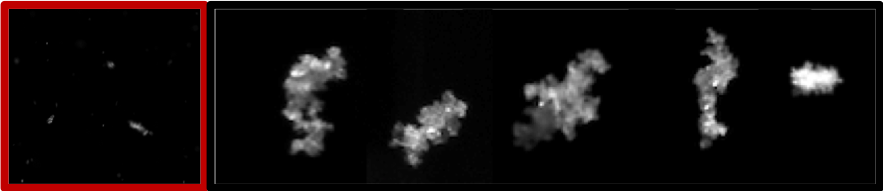
\includegraphics[width=0.8\textwidth]{./MASC_obs/blow_part}
	\caption{MASC observations during the Christmas storm 2016. Left (red frame), small ground up blowing snow particles. Five images on the right, rimed particles.}\label{fig:ret:all_part}
\end{figure}
%%%%%%%%%%%%%%%%%%%%%%%%%%%%%%%%%%%%%%%%%%%%%%
\noindent
The optimal estimation retrieval scheme was applied to the six-day Christmas 2016 storm event.  MASC images of snowfall during the event were used to guide the selection of the appropriate particle model and PSD input for the retrieval scheme. In this section, the sensitivity of retrieval results to these inputs is explored. Such an exercise should also allow an identification of those properties that yield the best match with Met-Norway snow gauge measurements at Haukeliseter.  
\\
The majority of the MASC images from Haukeliseter contained snow particles that looked like the left image \Cref{fig:ret:all_part} (red frame). Such images suggest small ground-up blowing snow particles that are consistent with the high winds observed during the event.  However, a careful examination of the MASC images also finds the presence of rimed aggregates such as those in the right five images (\Cref{fig:ret:all_part}). Pristine crystals such as plates and columns were not observed during the christmas 2016 event.  As such, the use of two different aggregate particle models developed for the CloudSat mission were explored. 
\\
\Cref{fig:ret_sensitivity} presents hourly measured snowfall accumulations on \SI{22}{\dec} plotted against retrieved values for the two different aggregate assumptions. The 'B8' aggregate is a low reflectivity per unit mass aggregate that worked well for the cold, dry conditions observed at Barrow as described in \citet{cooper_variational_2017}.  The 'B6' aggregate is a high reflectivity per unit mass particle.  As such, the 'B6' aggregate would seem more physically consistent with the observed rimed particles and high water environment found in the coastal mountains at Haukeliseter.  The presence of a water or rimed coating on the aggregates aloft would greatly enhance their effective reflectivity. Indeed, \Cref{fig:ret_sensitivity} suggests that the reflective 'B6' aggregate agreed much better than the less reflective 'B8' aggregate with the snow gauge.
%
\\
%%%%%%% image acc B6,B8 %%%%%%%%%%%%%%%%
\begin{figure}[t]
	\centering
	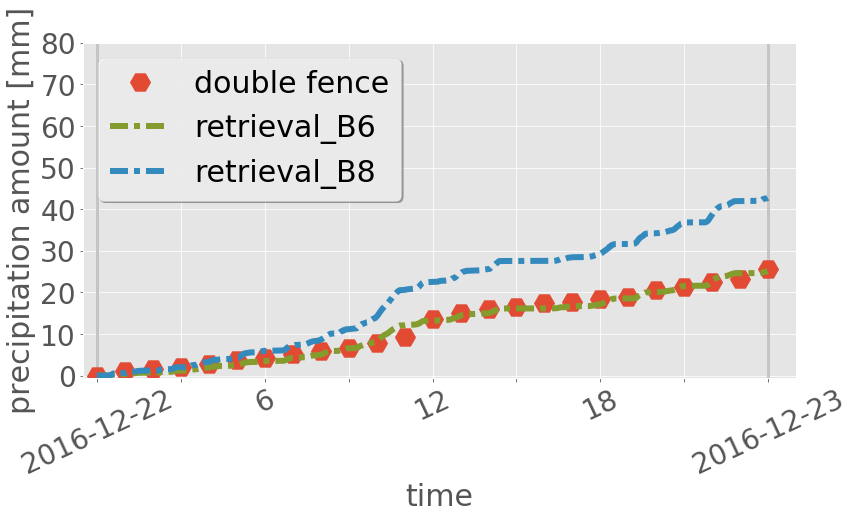
\includegraphics[width=0.8\textwidth]{./fig_obs_ret/20161222_2}
	\caption{Hourly double fence snowfall accumulations [mm] plotted against retrieved values for the \SI{22}{\dec} for different retrieval assumptions permutations. Double fence snowfall accumulation, red hexagons, retrieved precipitation amount for the here used study (B6), green, dash-dotted, and for small aggregates (B8), blue dashed.}\label{fig:ret_sensitivity}
\end{figure}
%%%%%%%%%%%%%%%%%%%%%%%%%%%%%%%%%%%%%%%%%%%%%%
\\
\Cref{tab:res:ret_sens} presents the percentage differences between snow gauge and retrieved estimates found when using these particle model assumptions for \SI{22}{\dec}. Use of the 'B6' aggregate agreed within \SI{5}{\percent} of the double fence observations (\Cref{tab:res:ret_sens}) for both \SI{12}{\hour} and \SI{24}{\hour} surface accumulations. Admittedly, use of the ‘B6’ aggregate produced slightly too little snowfall relative to the gauges for the remaining days of the event as discussed in \Cref{sec:ret_dofe_comp}. The use of the ‘B8’ aggregate, however, overestimated snowfall by at least \SI{65}{\percent} for both the \SI{12}{\hour} and \SI{24}{\hour} surface accumulations (\Cref{tab:res:ret_sens}). Since this aggregate had low reflectivity per unit mass, it required significantly more SWC in the forward model calculations to match MRR reflectivities. The retrieval therefore overestimates snowfall rate for these meteorological conditions.
\\
The discussion here has focused on MASC estimates of habit instead of PSD or fall speed. The reason is that the MASC and PIP saw primarily blowing snow particles at the surface that likely were much smaller than the particles that the MRR remotely sensed aloft.  The use of the PSD measured by the MASC or PIP in the retrieval therefore produced snowfall totals much greater than those measured by the double fence snow gauges.  Essentially, it takes a much greater mass of small particles than large particles to match a given reflectivity. These results contrast with those found for low wind speed events at Haukeliseter where the use of MASC habit, PSD, and fall speed observations resulted in retrieved snowfall accumulations very close to Met-Norway double fence gauge observations.  Regardless, for this high wind event, the \citet{wood_estimation_2011} a priori temperature PSD relationship and a climatological average fallspeed of \SI{0.85}{\mPs} \citep[private communication,][]{Priv_Comm_Schirle} were employed.
%%%%%%% table error sfc acc ret sensitivity %%%%%%%%%%%%%%%%
\begin{table}[t]
	\begin{center}
		\caption{Observations (obs.) and retrieved (ret.) snowfall amounts for \SI{22}{\dec} for different particle model assumptions. B6 indicating the here uses particle model (\Cref{app:scat_scheme}) and B8 indicating the retrieved snowfall amounts for small particles.}\label{tab:res:ret_sens}
		\begin{tabular}{c||r|r|c||r|r|c}
			\hline \hline
			& \multicolumn{3}{c||}{\textbf{\SI{12}{\hour} accumulation}} & \multicolumn{3}{c}{\textbf{\SI{24}{\hour} accumulation}}    \\\cline{2-7}
			\textbf{Particle} & \multicolumn{2}{c|}{\textbf{Snowfall}} & \textbf{Difference} &  \multicolumn{2}{c|}{\textbf{Snowfall}} & \textbf{Difference}   \\\cline{2-3} \cline{5-6}
			\textbf{model} & \textbf{obs.} & \textbf{ret.} && \textbf{obs.} & \textbf{ret.} &  \\\cline{2-7}
			& \multicolumn{2}{c|}{[\SI{}{\mm}]} & [\SI{}{\percent}]  & \multicolumn{2}{c|}{[\SI{}{\mm}]} & [\SI{}{\percent}]  \\ \hline\hline
			B6  & \num{13.6} &\num{13.2} & \num{-3.0} & \num{23.1} & \num{25.1} & \num{- 2.1}  \\\hline
			B8  & \num{13.6} &\num{22.5} & +\num{65.5} & \num{23.1} & \num{42.7} & +\num{66.9}  \\\hline\hline
		\end{tabular}
	\end{center}
\end{table}

%%%%%%%%%%%%%%%%%%%%%%%%%%%%%%%%%%%%%%%%%%%%%%%%%%%%%%%%%%%%%%%%%%%%%%%%%%
%

%%%%%%%%% Observation agreement %%%%%%%%%%%%%%
\subsection{Comparison of surface observations} \label{sec:ret_dofe_comp}
To be able to compare the vertical predicted snow water content with the retrieved snow water content a verification of the surface accumulation is made. If the retrieved surface accumulation is confident in comparison to the double fence measurement, then the vertical measurements can be trusted.
\\
The correlation in \Cref{fig:res:obs_ret_scatter} demonstrates a good agreement between the \SI{48}{\hour} accumulation measured by the double fence and the retrieved surface accumulation.
The black line in \Cref{fig:res:obs_ret_scatter} presents a linear correlation with a regression coefficient of R = \num{0.97}. 
In general, the retrieved surface snowfall accumulation is underestimated when compared to the double fence measurements, but not to a large degree. 
\\
\Cref{fig:res:diff_ret_scatter} shows the difference between retrieved accumulation and observed accumulation by the double fence. For the time period \num{20} to \SI{24}{\dec}, \Cref{fig:res:diff_ret_scatter} indicates an underestimation of retrieved snow accumulation of less than \SI{-5}{\mm} for the first \SI{24}{\hour}. 
Snow accumulation calculated on \SI{23}{\dec} at \SI{0}{\UTC} show after \SI{24}{\hour} an underestimation by the retrieval of up to \SI{-6.5}{\mm}. On \SI{24}{\dec}, larger underestimation after \SI{43}{\hour} is related to the observation of liquid precipitation on \SI{25}{\dec} between \SIrange{12}{21}{\UTC}. On \SI{25}{\dec} no fair comparison to the double fence measurement can be performed after \SI{12}{\UTC} because of the neglection of liquid precipitation when temperatures exceed \SI{2}{\celsius}.
\\
%The mean absolute difference of all days is \SI{2.06}{\mm} (excluding values on \SI{25}{\dec} after \SI{12}{\UTC} and on \SI{26}{\dec} after \SI{17}{\UTC} because of attenuation at the MRR). 
For a \SI{12}{\hour} accumulation follows for the Christmas storm (\num{21} to \SI{26}{\dec}) an average difference of \SI{85.5}{\percent} (\Cref{tab:res:ret_error}). For longer, \SI{24}{\hour} accumulation decreases the average difference to be \SI{- 4.7}{\percent} (excluding values on \SI{25}{\dec} after \SI{12}{\UTC} and on \SI{26}{\dec} after \SI{17}{\UTC} because of attenuation at the MRR). The daily surface snowfall accumulation difference between retrieval and observation in \Cref{tab:res:ret_error} show almost always a well agreement to the double fence. The only well pronounced mismatch is seen on \SI{21}{\dec}, where it measures much more than the double fence gauge (+\SI{435.8}{\percent}).
%%%%%%% image scatter obs ret %%%%%%%%%%%%%%%%
\begin{figure}[t]
	\centering
	\begin{subfigure}[b]{0.38\textwidth}
		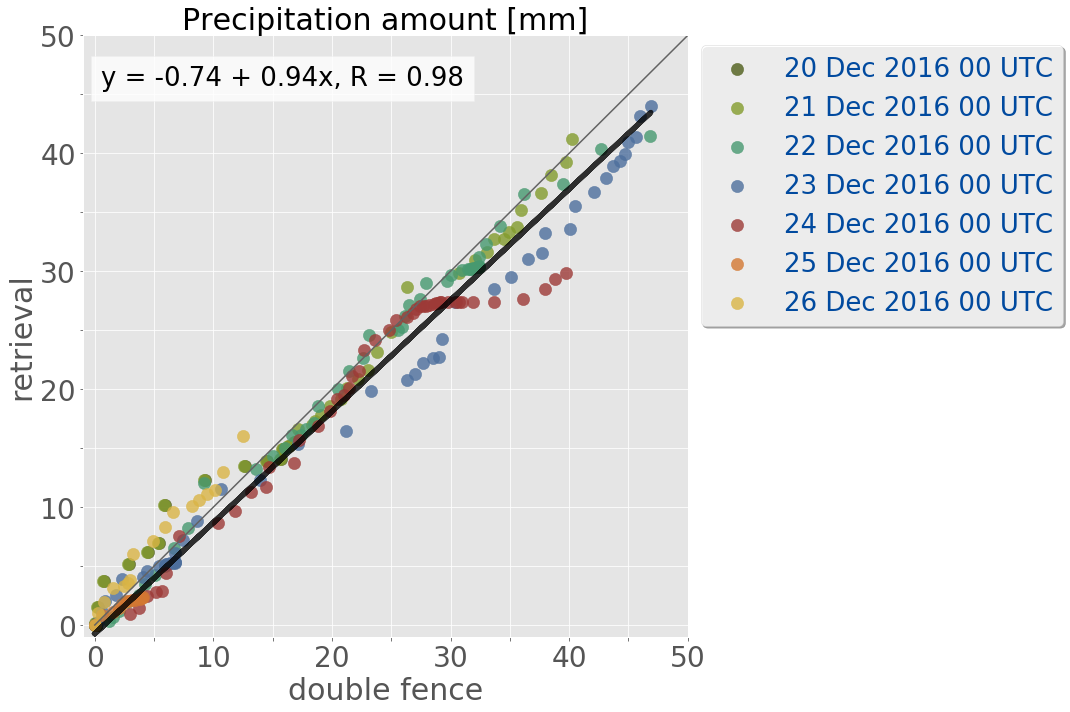
\includegraphics[trim={0.cm 0.cm 13cm 0cm},clip,
		width=\textwidth]{./fig_obs_ret/obs_ret_20161220_26_00}
		\caption{}\label{fig:res:obs_ret_scatter}
	\end{subfigure}
	%
	\begin{subfigure}[b]{0.59\textwidth}
		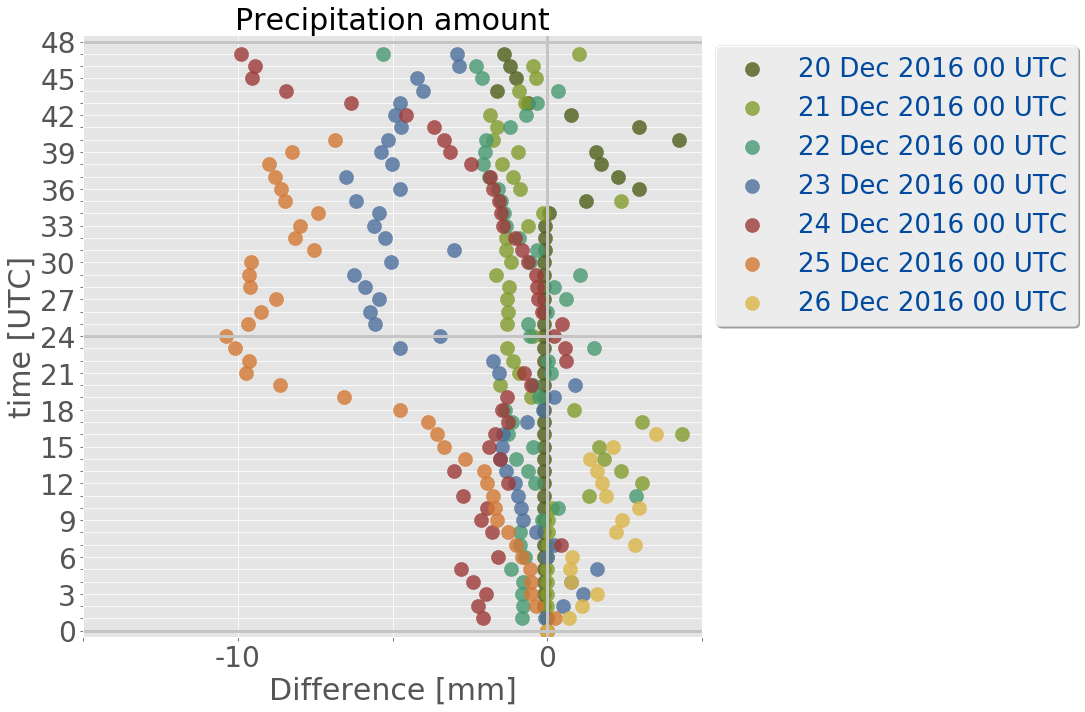
\includegraphics[trim={0.cm 0.cm 0cm 0cm},clip,
		width=\textwidth]{./fig_obs_ret/diff_20161220_26_00}
		\caption{}\label{fig:res:diff_ret_scatter}
	\end{subfigure}
	% label
	%    \begin{subfigure}[t]{0.18\textwidth}
	%   	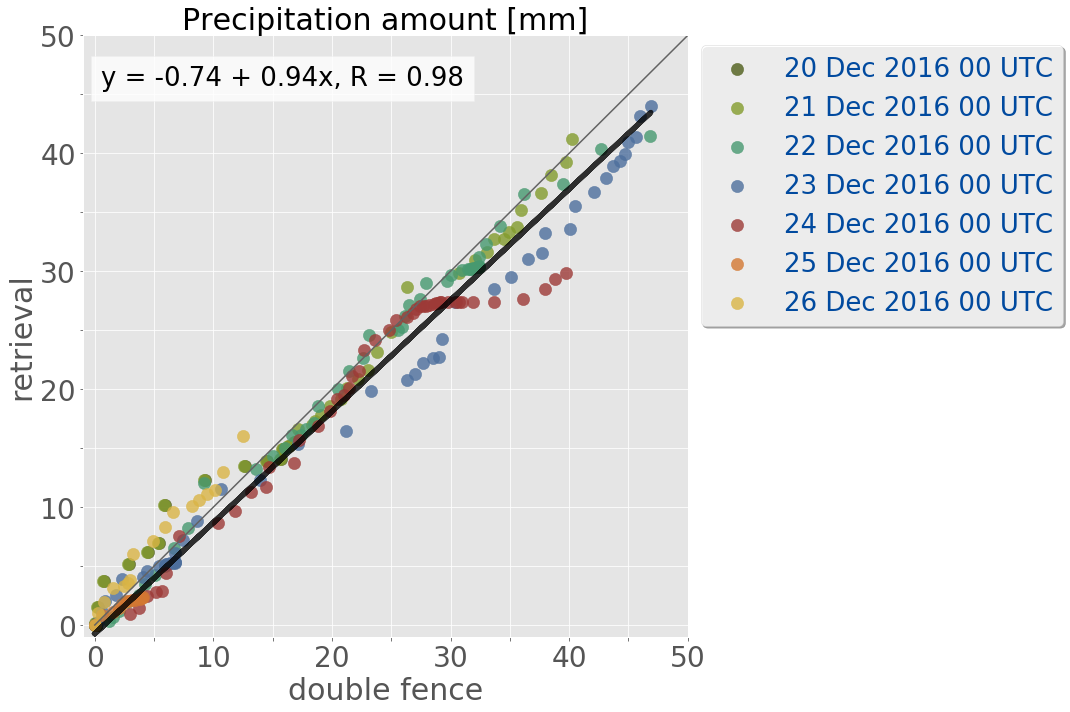
\includegraphics[trim={25.cm 13.cm 0cm 1.3cm},clip,
	%  width=\textwidth]{./fig_obs_ret/obs_ret_20161220_26_00}
	% \end{subfigure}
	\caption{\protect\subref{fig:res:obs_ret_scatter}: Surface precipitation amount comparison between the double fence observations and the retrieved surface accumulation of precipitation for \SI{48}{\hour}. In black the linear correlation between the double fence observations and retrieved surface snow. 
		\protect\subref{fig:res:diff_ret_scatter}: Difference between the retrieved and the observed accumulation by the double fence. The colours represent the different starting days at \SI{0}{\UTC} for the \SI{48}{\hour} accumulation.}\label{fig:res:obs_ret}
\end{figure}
%%%%%%%%%%%%%%%%%%%%%%%%%%%%%%%%%%%%%%%%%%%%%%
\\
\\
Similar to this study, \citet{cooper_variational_2017} used a CloudSat snow particle model, PSD and fall speed from MASC observations for five snow events at Barrow, Alaska. The comparison to the weather station revealed an difference between National Weather Service observations and retrieved accumulations of \SI{- 18}{\percent} for five snow events.
%%%%%%% table error sfc acc ret obs %%%%%%%%%%%%%%%%
\begin{table}[t!]
	\begin{center}
		\caption{Comparison of observed (obs.) and retrieved (ret.) snowfall amounts for the Christmas storm 2016. Difference refers to the difference of the retrieved and observed snow accumulation after \SI{12}{\hour} and \SI{24}{\hour}. The average difference is the value over all six/four days. Excluding values after \SI{12}{\UTC} on \SI{25}{\dec} and after \SI{17}{\UTC} on \SI{26}{\dec}.}\label{tab:res:ret_error}
		\begin{tabular}{c||r|r|c|c||r|r|c|c}
			\hline \hline
			& \multicolumn{4}{c||}{\textbf{\SI{12}{\hour} accumulation}} & \multicolumn{4}{c}{\textbf{\SI{24}{\hour} accumulation}}    \\ \cline{2-9}
			\textbf{Day} & \multicolumn{2}{c|}{\textbf{Snowfall}} & \textbf{Difference} & \textbf{Average} &  \multicolumn{2}{c|}{\textbf{Snowfall}} & \textbf{Difference} & \textbf{Average}  \\\cline{2-3} \cline{6-7}
			\textbf{in 2016} & \textbf{obs.} & \textbf{ret.} & & \textbf{difference} & \textbf{obs.} & \textbf{ret.} & & \textbf{difference} \\\cline{2-9}
			& \multicolumn{2}{c|}{[\SI{}{\mm}]} & [\SI{}{\percent}] & [\SI{}{\percent}] & \multicolumn{2}{c|}{[\SI{}{\mm}]} & [\SI{}{\percent}] & [\SI{}{\percent}] \\ \hline\hline
			\num{20} Dec & \num{0.1} &\num{0.0} & \num{-97.8} & & \num{0.1} & \num{0.0} & \num{- 97.8} &  \\\cline{1-9}
			\num{21} Dec & \num{0.7} & \num{3.8} & +\num{435.8} &  & \num{17.1} & \num{16.6} & \num{-2.7} & \multirow{4}{*}{\num{-4.7}}   \\\cline{1-5}\cline{6-8}
			\num{22} Dec & \num{13.6}& \num{13.2} & \num{- 3.0} & \multirow{5}{*}{\num{-2.1}} & \num{25.6} &\num{25.1} & \num{-2.1} &   \\\cline{1-4}\cline{6-8}
			\num{23} Dec & \num{6.3} &\num{5.2} & \num{- 16.8} & & \num{23.3}& \num{19.8} & \num{-14.9} &   \\\cline{1-4}\cline{6-8}
			\num{24} Dec & \num{14.7} & \num{13.4} & \num{- 8.6} && \num{24.8} & \num{25.0} & +\num{0.8} &   \\\cline{1-4}\cline{6-9}
			\num{25} Dec &  \num{4.3} & -- & -- & & +\num{15.4} & -- & -- & \\\cline{1-4}\cline{6-9}
			\num{26} Dec & \num{8.8} & \num{10.6} & +\num{20.1} &  &  \num{25.1} &-- & -- &  \\\hline\hline
		\end{tabular}
	\end{center}
\end{table}
%%%%%%%%%%%%%%%%%%%%%%%%%%%%%%%%%%%%%%%%%%%%%%
\\
\Cref{tab:res:ret_error} shows the difference for each individual day and the average difference for six and four days, depending on the accumulation of \SI{12}{\hour} or \SI{24}{\hour}.
The choice of the correct PSD model, slope parameters and fall speed in the optimal estimation snowfall retrieval, shows a good agreement with the observations at Haukeliseter for the 2016 Christmas storm in contrast to the \SI{200}{\percent} difference when only using the CloudSat snowfall algorithm (\Cref{sec:retrieval}). It indicates also a reduction of the non-uniqueness of snow accumulation is reduced, when using a combination of ground-based observations instead of only Ze-S relationships. 
%Of course, more storms should be investigated to find the exact correlation between the surface observations and the estimated accumulation to see if the deviation keeps as small for different snow patterns at Haukeliseter. 
%During the 2016 Christmas storm the average error for \SI{24}{\hour} accumulation is almost similar to the best estimate at Barrow, Alaska. 
\\
It turns out that there is no relation between high and low precipitation events since the differences vary daily. \citet{cooper_variational_2017} showed also different combinations of PSD assumptions and snow fall speed. For Barrow, best agreements between observations and retrieved snowfall were found by using the CloudSat particle model, slope parameters and snowfall speeds from the MASC. In the here presented study, the best assumption for surface snowfall accumulation was found by using a particle model for rimed aggregates (\Cref{sec:retrieval} and \ref{sec:ret:sensitivity}) such as in \Cref{fig:ret:all_part}. 
\\
\\
On \num{20} and \SI{21}{\dec}, the difference error is large (\SI{-97.8}{\percent} and \SI{435.8}{\percent}, respectively). This is probably related to an observation of precipitation at the double fence, even though no precipitation was observed. 
On \SI{20}{\dec}, observation at the double fence might be related to some particles stirred up by wind into the orifice of the gauge. Since no manual observations are done at the Haukeliseter site, is it difficult to say if blowing snow occurred or if it was snowing. This introduces additional errors on the double fence measurements. From the vertical MRR reflectivity, in \Cref{sec:res:large_scale_vert}, \Cref{fig:ret:refl}, it can be seen, that precipitation was not observed on \SI{21}{\dec} before \SI{9}{\UTC}.
\\
Even though it is assumed that the double fence is the correct measurement it still underlies some uncertainties, such as under-catch during high wind speeds \citep{wolff_wmo_2018}. 
A better way to asses the accuracy of the retrieved surface snowfall accumulation could be to compare the results to measurements inside a bush gauge. 
\\
\citet{wolff_wmo_2018} estimates the under-catchment of double fence gauge compared to bush gauge measurements to \SI{10}{\percent}, for outside winds of \SI{9}{\mPs} (\Cref{sec:dofe}).
If the double fence gauge underestimate snowfall under high wind condition, would follow that the optimal estimation retrieval results are more than \SI{20}{\percent} too low to the true state. 
\\
Anyway, the low average difference value for \SI{24}{\hour} accumulation, in \Cref{tab:res:ret_error} during the Christmas 2016 event (\SI{-4.7}{\percent}) follow a much lower average difference between retrieved and observed surface accumulation than at Barrow (\SI{36}{\percent}) and therefore a very good agreement between observed and retrieved snow accumulation during \num{21} to \SI{24}{\dec}. In \Cref{sec:res:large_scale_vert}, the vertical SWC will be compared to the forecasted MEPS values for the 2016 Christmas storm. Despite the undercatchment of wind related snow precipitiation, the double fence measurement give confidence for the retrieved profiles of snow water content. While snow water content is compared to the MEPS forecast, it should be kept in mind that retrieved snow accumulation is underestimated and therefore the vertical SWC may be too low.
%influenced by wind will the small average difference for \num{21} to \SI{24}{\dec} give confidence in the retrieved profiles of snow water content when comparing to the forecast, but it should be kept in mind that retrieved snow accumulation is underestimated and therefore may the vertical SWC be too low.
%%%%%%%%%%%%%%%%%%%%%%%%%%%%%%%%%%%%%%%%%%%%%%%%%%%%%%%%%%%%%%%%%%%%%%%%%%


%%%%%%%%%%%%%%%%%%%%%%%%%%%%%%%%%%%%%%%%%%%%%%%%%%%%%%%%%%%%%%%%%%%%%%%%%
%%%%%%%% Overestimation of surface snowfall %%%%%%%%%%%%%%
\subsection{MEPS forecast and surface observation comparison}\label{sec:sfc_acc}
One approach of this study is to see if observed surface accumulation was correctly predicted by the newly operational regional weather forecast model MEPS (\Cref{sec:DIM:MEPS}). 
%precipitation amount at the surface are shown in \Cref{fig:sfc_acc}. 
%The figures are representing the observed and forecasted surface precipitation accumulation in \SI{}{\mm} over \SI{48}{\hour}. 
\Cref{fig:sfc_acc} shows observations at the double fence, retrieved snow accumulation, and MEPS forecast for \SI{48}{\hour}. Hereafter, MEPS surface precipitation prediction forecast is compared to the double fence gauge observations at Haukeliseter. 
Accumulation measured by the double fence are presented as red hexagons. Minutely retrieved surface snowfall amount in dash-dotted green. Lines in black and grey show the deterministic and perturbed members for lead time of \SI{48}{\hour}
%The ten \SI{48}{\hour} forecast ensemble members are lines in black and grey, the deterministic and its perturbed ensemble members, respectively. 
The blue dashed line shows the ensemble mean of all ten members. The ensemble mean of precipiation amount is calculated every three hours, due to the three hourly time resolution of most of the perturbed member.
%Since the deterministic and the first ensemble member have values every hour and the other perturbed members only every three hours, shows the ensemble mean the precipitation amount  every \SI{3}{\hour} forecast time. 
When not all perturbed member data was available from \citet{norwegian_meteorological_institute_met_2016}, like on \SI{23}{\dec} (\Cref{fig:sfc_acc23}), no ensemble mean is calculated. 
At the bottom of \Cref{fig:sfc_acc} the associated \SI{10}{\minute} average wind of the last hour from the \SI{10}{\metre} weather mast at Haukeliseter is presented, to see if surface accumulation observations may be influenced by wind. 
\\
In general, \Cref{fig:sfc_acc21,fig:sfc_acc22,fig:sfc_acc23} show a better agreement between double fence observations and forecast for \SI{48}{\hour} forecasts initialised on \num{21} to \SI{23}{\dec} at \SI{0}{\UTC}. 
%The spread of the ensemble members around the control run fit better to the observations as well than initialisations on \num{24} to \SI{26}{\dec}. 
The double fence observation lie for \num{21}, \num{22}, and \SI{23}{\dec} within the spread of the ensemble members (\Cref{fig:sfc_acc21,fig:sfc_acc22,fig:sfc_acc23}), covering the uncertainty within the measurements (\Cref{sec:DIM:MEPS}). On the other hand, observations between \num{24} and \SI{26}{\dec} are too low  compared to the ensemble spread (\Cref{fig:sfc_acc24,fig:sfc_acc25,fig:sfc_acc26}).
During \num{24} and \SI{26}{\dec}, the low-pressure system intensifies and gets closer to the Norwegian coast, and influence the local weather in Norway (\Cref{sec:largeScale}). \Cref{fig:sfc_acc24}, \subref{fig:sfc_acc25}, and \subref{fig:sfc_acc26} indicate a larger estimated surface precipitation amount for all ten ensemble members compared to observed values at the measurement site between \num{24} to \SI{26}{\dec}. 
\\ 
\\
%%% image surface accumulation %%%%%%%%%%%%%%%%%%%%%%%%%%%%%%%%%%%%%
\begin{figure}[H]
	\centering
	% 21/12
	\begin{subfigure}[t]{0.85\textwidth}		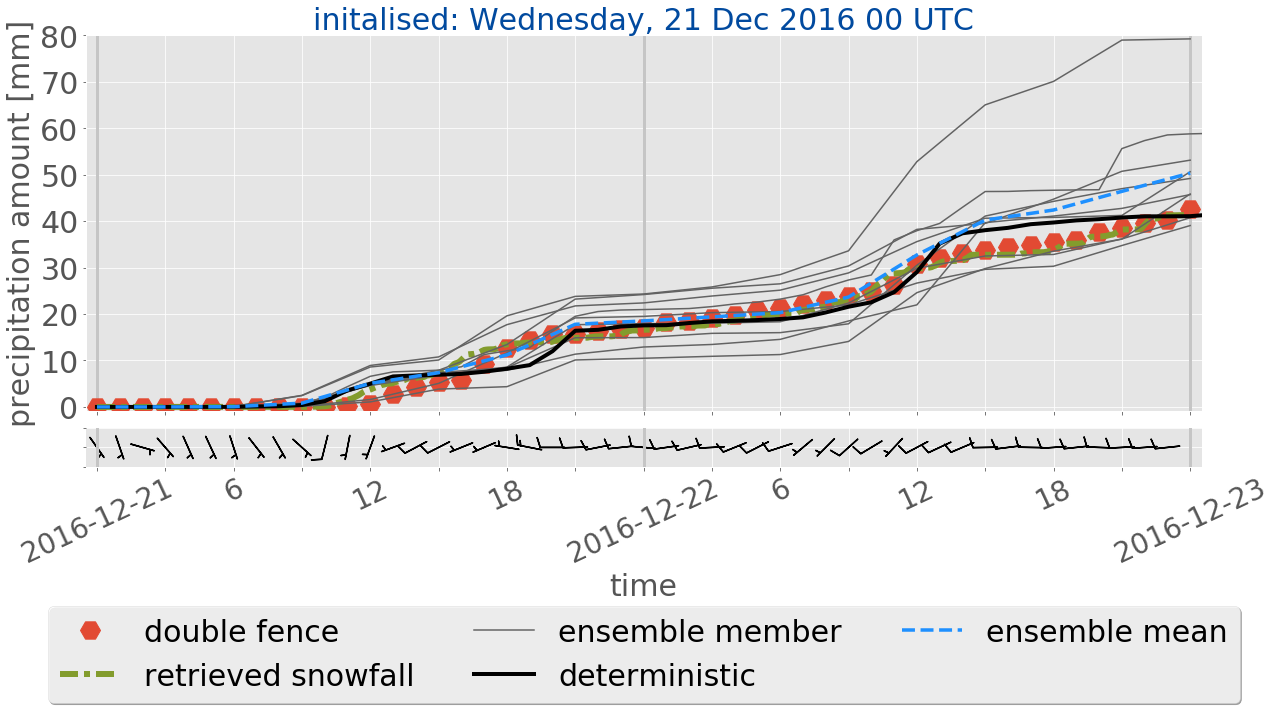
\includegraphics[trim={0.cm 5.2cm 0.cm 0cm},clip,width=\textwidth]{./fig_sfc_acc/acc_wind_20161221_00}
		\caption{}\label{fig:sfc_acc21}
	\end{subfigure}
	% 22/12
	\begin{subfigure}[t]{0.85\textwidth}		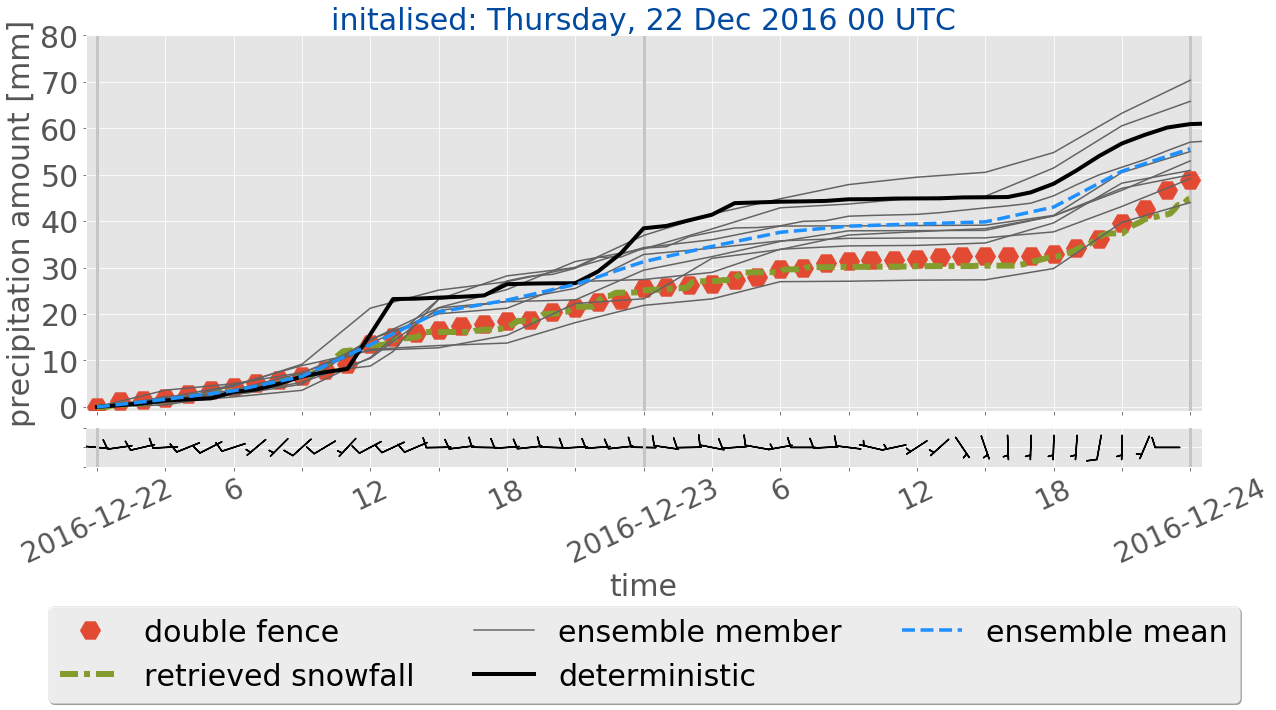
\includegraphics[trim={0.cm 5.2cm 0.cm 0cm},clip,width=\textwidth]{./fig_sfc_acc/acc_wind_20161222_00}
		\caption{}\label{fig:sfc_acc22}
	\end{subfigure}
	% label
	\begin{subfigure}[t]{\textwidth}
		\centering
		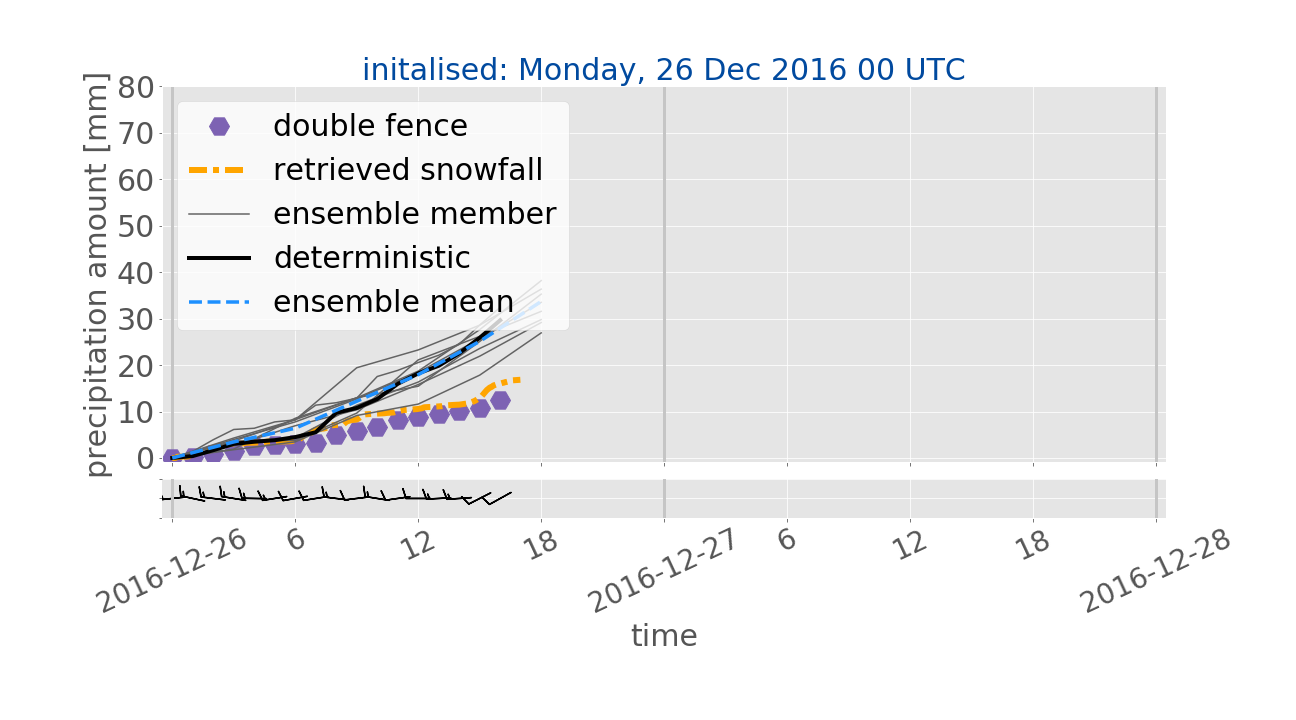
\includegraphics[trim={1.2cm 0cm 1.1cm 21.4cm},clip,width=0.8\textwidth]{./fig_sfc_acc/acc_wind_20161226_00}
	\end{subfigure}
	\caption{\SI{48}{\hour} surface snowfall accumulation for \num{21} to \SI{26}{\dec} (\protect\subref{fig:sfc_acc21} to \protect\subref{fig:sfc_acc26}). Representing the values from the double fence in red, hexagons; optimal estimation retrieval output at the first noise free level
		%snow layer height \SI{400}{\metre} 
		in dash-dotted green; MEPS ensemble member deterministic forecast, initialised at \SI{00}{\UTC} in black and its nine perturbed ensemble members in grey. The ensemble mean of all ten members is shown in dashed blue. Underneath is the associated last hour \SI{10}{\minute} average wind from the weather mast at \SI{10}{\metre} height. \textit{Continued on next page.}}\label{fig:sfc_acc}
\end{figure}
\begin{figure}[H]\ContinuedFloat
	\centering
	% 23/12
	\begin{subfigure}[t]{0.85\textwidth}	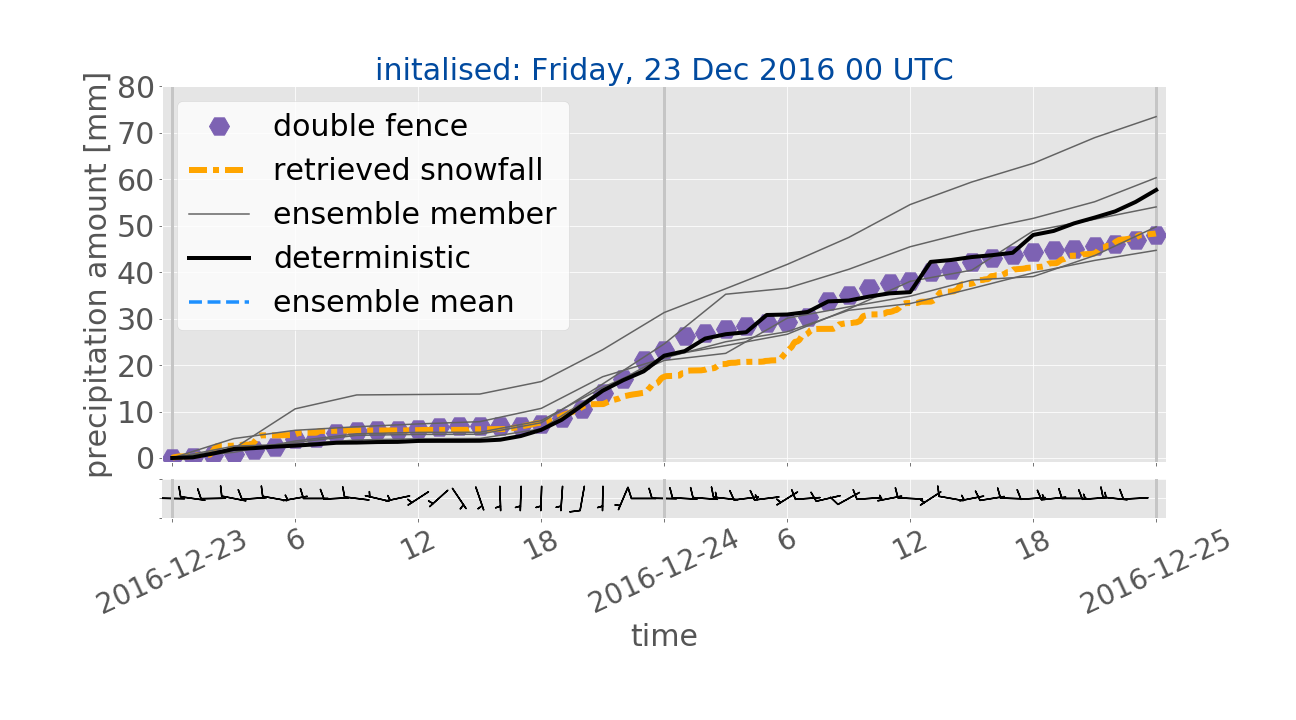
\includegraphics[trim={0.cm 5.2cm 0.cm 0cm},clip,width=\textwidth]{./fig_sfc_acc/acc_wind_20161223_00}
		\caption{}\label{fig:sfc_acc23}
	\end{subfigure}
	% 24/12
	\begin{subfigure}[t]{0.85\textwidth}			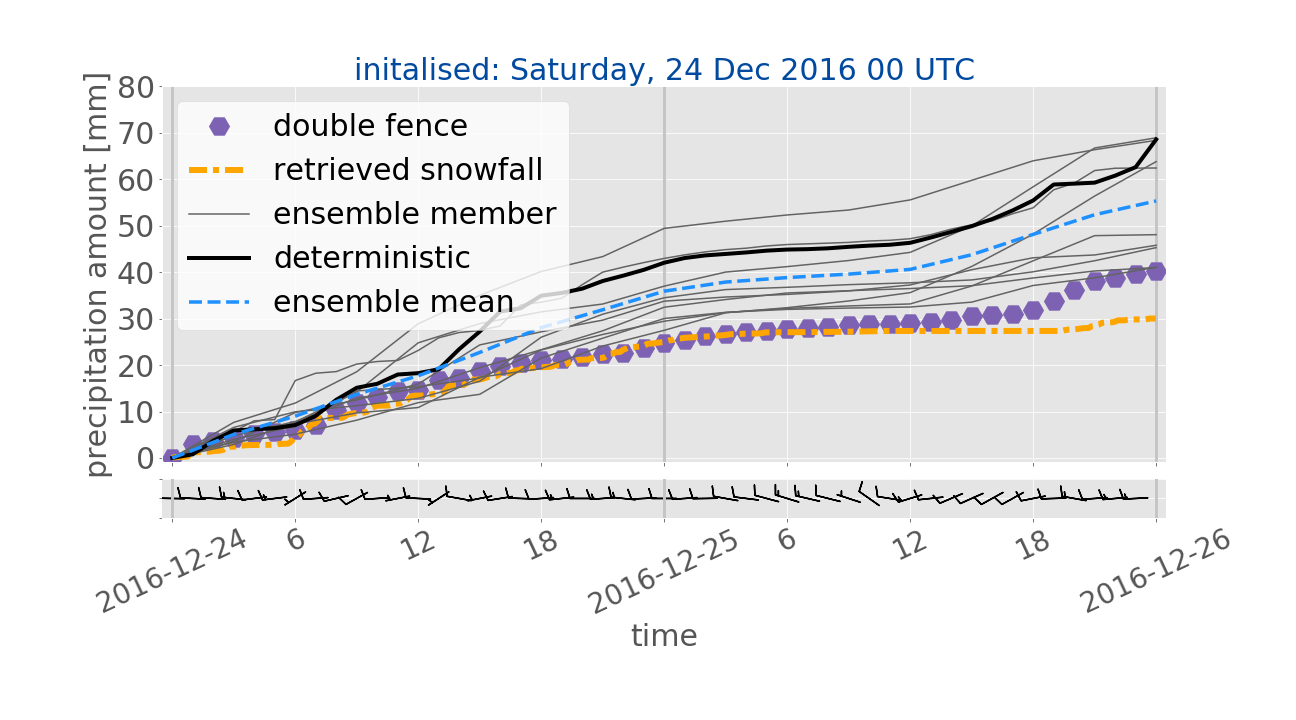
\includegraphics[trim={0.cm 5.2cm 0.cm 0cm},clip,width=\textwidth]{./fig_sfc_acc/acc_wind_20161224_00}
		\caption{}\label{fig:sfc_acc24}
	\end{subfigure}
	% 25/12
	\begin{subfigure}[t]{0.85\textwidth}
		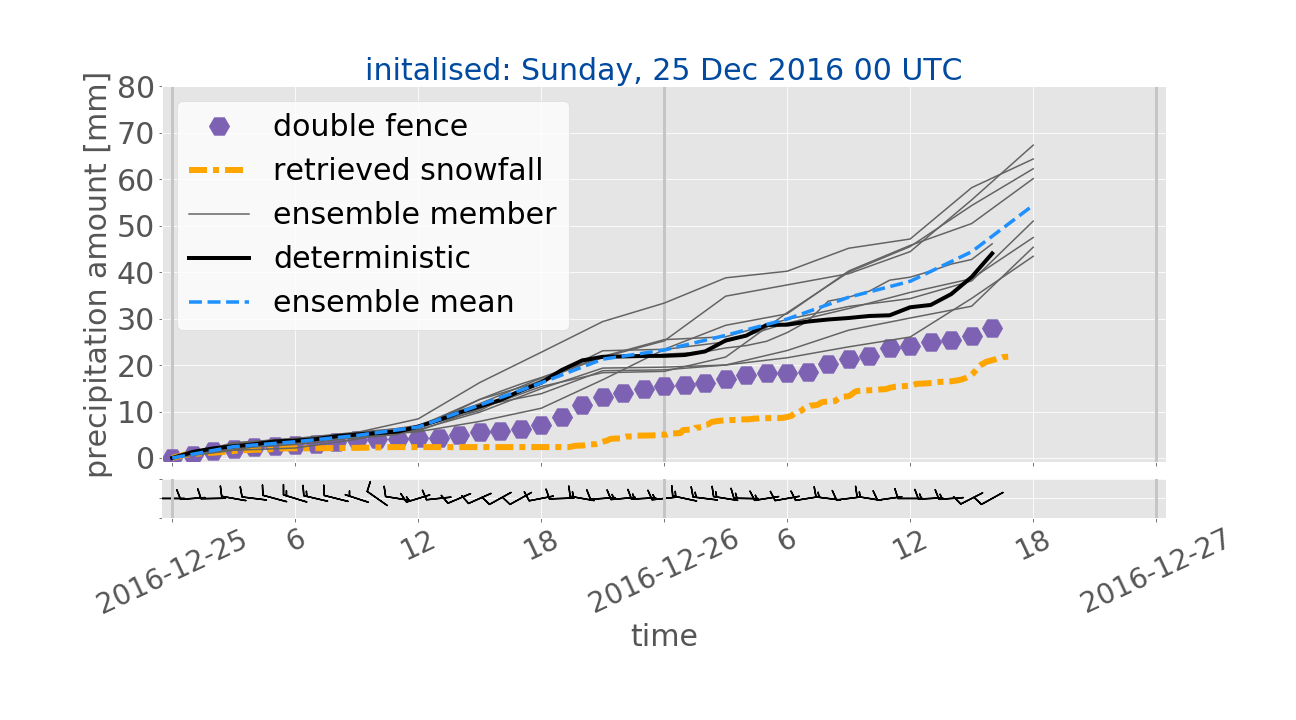
\includegraphics[trim={0.cm 3.6cm 0.cm 0cm},clip,width=\textwidth]{./fig_sfc_acc/acc_wind_20161225_00}
		\caption{}\label{fig:sfc_acc25}
	\end{subfigure}
	% label
	\begin{subfigure}[t]{\textwidth}
		\centering
		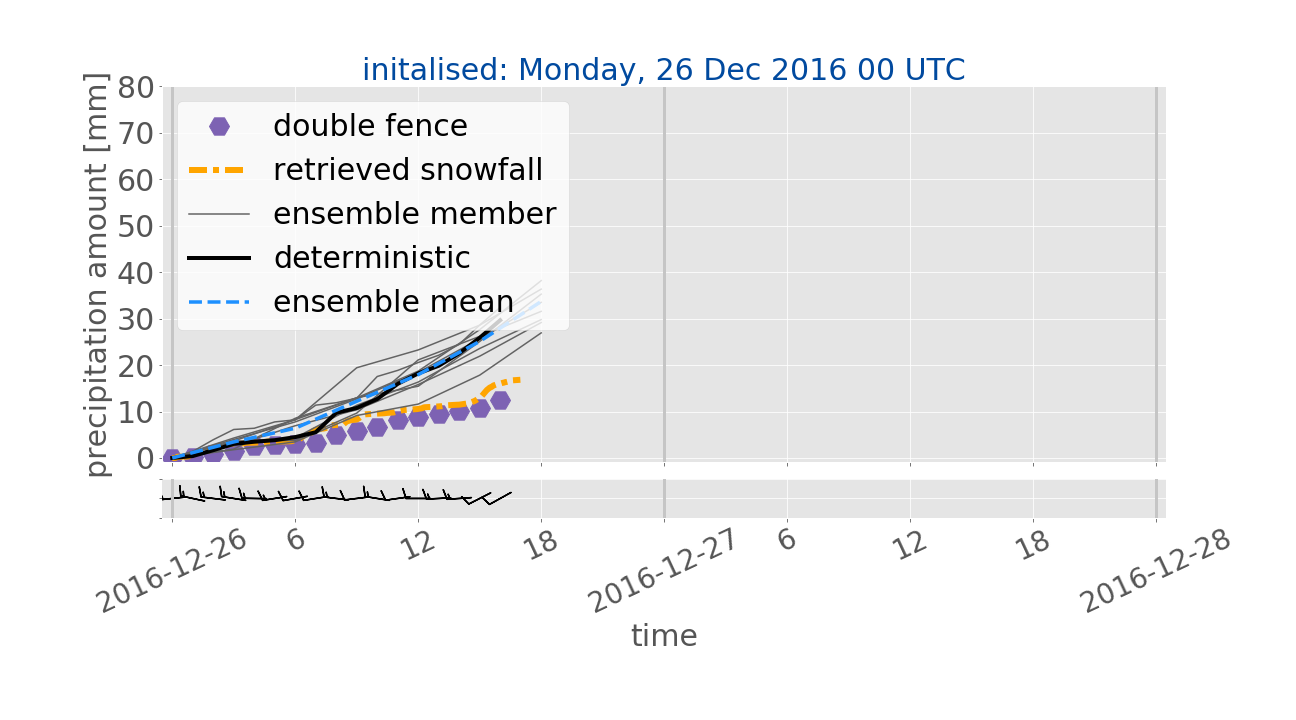
\includegraphics[trim={1.2cm 0cm 1.1cm 21.4cm},clip,width=0.8\textwidth]{./fig_sfc_acc/acc_wind_20161226_00}
	\end{subfigure}
	\caption{\textit{(Continued from previous page.)} }
\end{figure}
\begin{figure}[H]\ContinuedFloat
	\centering
	% 26/12
	\begin{subfigure}[t]{0.85\textwidth}	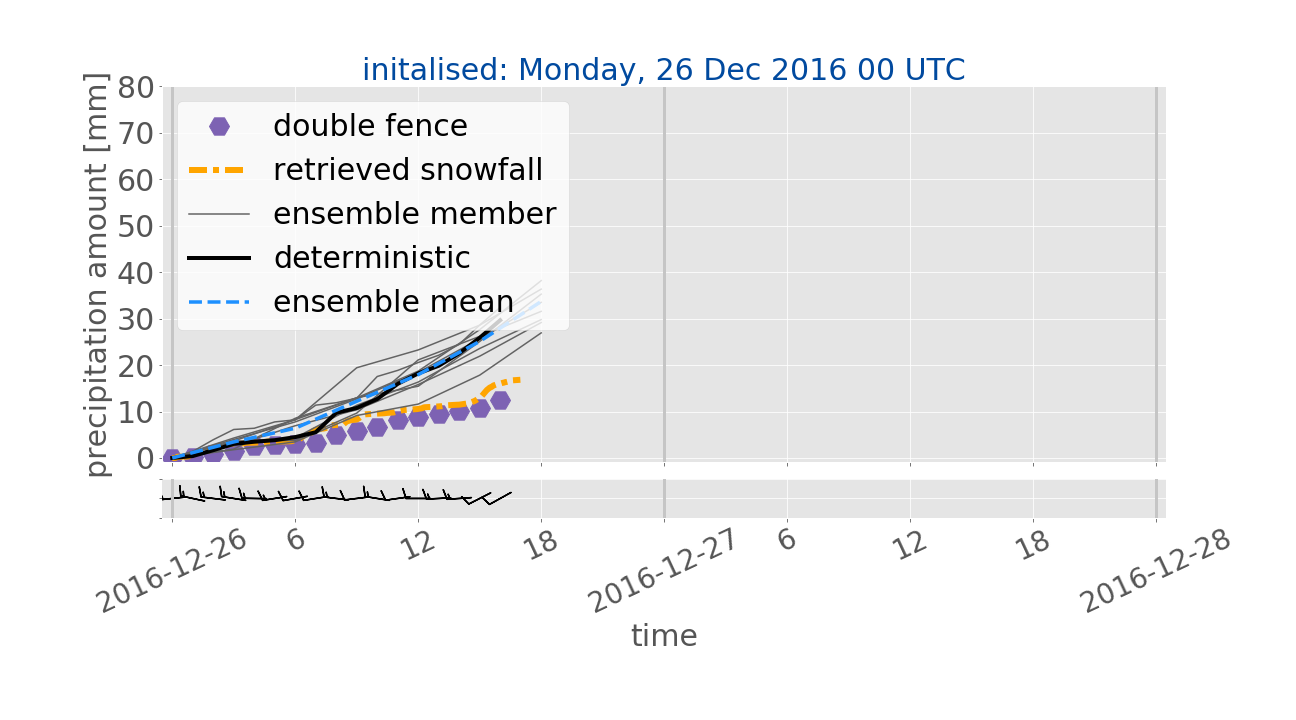
\includegraphics[trim={0.cm 3.6cm 0.cm 0cm},clip,width=\textwidth]{./fig_sfc_acc/acc_wind_20161226_00}
		\caption{}\label{fig:sfc_acc26}
	\end{subfigure}
	%	
	% label
	\begin{subfigure}[t]{\textwidth}
		\centering
		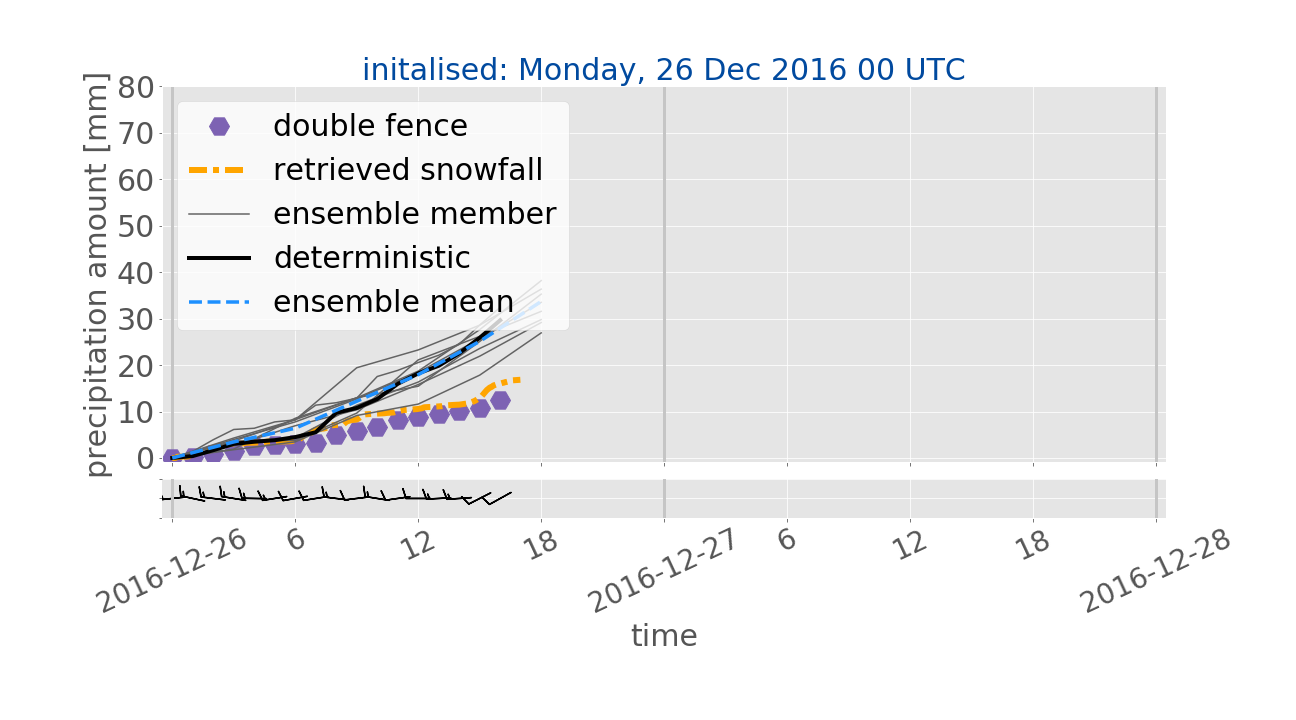
\includegraphics[trim={1.2cm 0cm 1.1cm 21.4cm},clip,width=0.8\textwidth]{./fig_sfc_acc/acc_wind_20161226_00}
	\end{subfigure}
	\caption{\textit{(Continued from previous page.)} }
\end{figure}
%%%%%%%%%%%%%%%%%%%%%%%%%%%%%%%%%%%%%%%%%%%%%%%%%%%%%%%%%%%%%%%%%%%%%%%%%%
\noindent
The correlation between \SI{48}{\hour} double fence observation and ensemble precipitation forecast is presented in \Cref{fig:scat:pres2123} and \subref{fig:scat:pres2426}. Showing a better agreement for \num{21} to \SI{23}{\dec} than initialisation on \num{24} to \SI{26}{\dec}. On \num{21} to \SI{23}{\dec} the slope of the regression line is relatively close to unity, indicating a good agreement between MEPS forecast and the observations by the double fence.
The largest disagreement between surface observations and forecasts is seen on \SI{25}{\dec} with a wet bias up to \SI{15}{\mm} (\Cref{fig:bias:precip12}). The mean absolute error is not larger than \SI{13}{\mm} for the first three days and increases with intensification of the storm up to \SI{19}{\mm} on \SI{24}{\dec}.
\\
Initialisations on \SI{24}{\dec} (\Cref{fig:sfc_acc24}) indicate an overestimation of the deterministic surface snowfall prediction already after \SI{13}{\hour} forecast time. The deterministic forecast in solid black is much higher and increases faster than the observations. In \Cref{fig:sfc_acc24} at \SI{16}{\UTC} a difference of approximately \SI{15}{\mm} can be seen when compared to the surface measurements. This difference remains almost constantly over the forecast time. Furthermore, all ensemble members seem to overestimate the surface accumulation after \SI{24}{\hour}. 
\\
Since MEPS performance was better on the previous days one might assume that the double fence measurement is influenced by surface winds. It shows in \Cref{fig:sfc_acc24} that the \SI{10}{\minute} average wind at \SI{13}{\UTC} increases from \SI{5}{\mPs} to \SI{10}{\mPs} (see also \Cref{fig:res:sfc_ws23}). \citet{wolff_wmo_2018} states that the double fence gauge is influenced by wind, and that the double fence gauge underestimates precipitation accumulation within \SI{10}{\percent} for winds up to \SI{9}{\mPs}.
%but accumulation measurement errors occur rather at higher wind speeds larger than \SI{20}{\mPs}. It is therefore assumed that the measurements from the double fence are correct and MEPS had rather a forecasting issue.
%%%%%%% table error MEPS accumulation %%%%%%%%%%%%%%%%
\begin{table}[t]
	\begin{center}
		\caption{Observations (obs.) and forecasted (MEPS) snowfall amounts for the Christmas storm 2016. Difference refers to the percentage difference between MEPS ensemble members and the double fence observation, averaged over all ensemble member for \SIlist{12;24}{\hour}. The average difference is the value over all days.}\label{tab:res:MEPS_err}
		\begin{tabular}{c||r|r|c|c|c||r|r|c|c|c}
			\hline \hline
			& \multicolumn{5}{c||}{\textbf{\SI{12}{\hour} accumulation}} & \multicolumn{5}{c}{\textbf{\SI{24}{\hour} accumulation}}    \\ \cline{2-11}
			\textbf{Day} & \multicolumn{2}{c|}{\textbf{Snowfall}} & \textbf{Difference} & \multicolumn{2}{c||}{\textbf{Average}} &  \multicolumn{2}{c|}{\textbf{Snowfall}} & \textbf{Difference} & \multicolumn{2}{c}{\textbf{Average}}  \\\cline{2-3} \cline{7-8}
			\textbf{in 2016} & \textbf{obs.} & \textbf{MEPS} & & \multicolumn{2}{c||}{\textbf{difference}} & \textbf{obs.} & \textbf{MEPS} & & \multicolumn{2}{c}{\textbf{difference}} \\\cline{2-11}
			& \multicolumn{2}{c|}{[\SI{}{\mm}]} & [\SI{}{\percent}] & \multicolumn{2}{c||}{ [\SI{}{\percent}]} & \multicolumn{2}{c|}{[\SI{}{\mm}]} & [\SI{}{\percent}] & \multicolumn{2}{c}{ [\SI{}{\percent}]} \\ \hline\hline
			\num{20} Dec & \num{0.1} &\num{0.4} & +\num{290.7} & & &\num{0.1} & \num{0.4} & +\num{302.1} & & \\\cline{1-11}
			\num{21} Dec & \num{0.7} & \num{5.1} & +\num{626.1} &  &\multirow{6}{*}{+\num{134.7}} & \num{17.1} & \num{18.5} & +\num{8.3} & \multirow{3}{*}{+\num{10.8}}& \multirow{6}{*}{+\num{32.6}}   \\\cline{1-5}\cline{7-9} 
			\num{22} Dec & \num{13.6} & \num{13.4} & \num{-1.6} & \multirow{2}{*}{+\num{1.3}} & & \num{25.6} & \num{31.3} & +\num{22.2} &  &  \\\cline{1-4}\cline{7-9}
			\num{23} Dec & \num{6.3} & \num{6.6} & +\num{4.2} & & & \num{23.3} & \num{23.7} & +\num{1.8} &  &  \\\cline{1-5}\cline{7-10}
			\num{24} Dec & \num{14.7} & \num{17.7} & +\num{20.4} & \multirow{3}{*}{+\num{59.8}} & & \num{24.8} & \num{35.9} & +\num{44.8} & \multirow{3}{*}{+\num{54.4}}  &  \\\cline{1-4}\cline{7-9}
			\num{25} Dec & \num{4.3} & \num{6.7} & +\num{55.1} & & & \num{15.4} & \num{23.3} & +\num{50.8} & &   \\\cline{1-4}\cline{7-9}
			\num{26} Dec & \num{8.8} & \num{17.9} & +\num{104.0} & & & \num{25.1} & \num{42.1} & +\num{67.5} &  &  \\\hline\hline
		\end{tabular}
	\end{center}
\end{table}
%%%%%%%%%%%%%%%%%%%%%%%%%%%%%%%%%%%%%%%%%%%%%%%%%%%%%%%%%%%%%%%%%%%%%%%%%%
\Cref{tab:res:MEPS_err} shows the difference between the observations and ensemble mean MEPS forecast for \SIlist{12;24}{\hour}. As seen in \Cref{tab:res:MEPS_err}, the average difference error decreases with longer forecast time. 
For \num{21} to \SI{26}{\dec} the average difference error is +\SI{134.7}{\percent}. For longer lead times, \SI{24}{\hour}, the average difference error is reduced to +\SI{32.6}{\percent}. The daily percent difference show to be high for the last three days of the 2016 Christmas extreme event. On \SI{21}{\dec} very large difference error (\SI{626.1}{\mm}) is shown. This error is related to the small precipitation amount (\SI{0.7}{\mm}) observations at Haukeliseter, which is a known difficulty for precipitation forecasts \citep{muller_arome-metcoop:_2017}. Generally the forecast accuracy decreases with lead time \citep{kalnay_atmospheric_2003}.
\\
\\
While the cyclone moves closer to Norway, the forecast inaccuracy of the surface precipitation increases. Overestimation occures around \SI{12}{\UTC} on \SI{25}{\dec}. This overestimation of the precipitation amount could be associated with the warm sector evolution at Haukeliseter (\Cref{sec:res:large_scale_sfc}). Afterwards it shows, with increasing lead time the same accumulation is predicted, but too high compared to the double fence observations.
%Afterwards, the model follows the same path as the double fence observations, but higher. The MEPS forecast on \SI{25}{\dec} indicates a good spread between the ensemble members and the deterministic forecast, while on \SI{24}{\dec} the ensemble member were not spread symmetrically around the deterministic forecast. On \SI{25}{\dec}, the difference between \SI{12}{\hour} accumulation observations and MEPS forecast is \SI{55.1}{\percent} (\Cref{tab:res:MEPS_err}). 
The wind at Haukeliseter was higher than \SI{10}{\mPs} (\Cref{fig:sfc_acc25} before \SI{12}{\UTC}. A realtion between high wind and double fence observation could be possible. Assuming an accumulation underestimation of \SI{10}{\percent} would lead to a reduciton of overestiatmon to \SI{40.2}{\percent} for \SI{12}{\hour} (\Cref{tab:res:MEPS_err_10}).
%%%%%%% table if 10% underestimate of double fence %%%%%%%%%%%%%%%%
\begin{table}[t]
	\begin{center}
		\caption{Same as \Cref{tab:res:MEPS_err}, just for an under-catchment of \SI{10}{\percent} difference by the double fence gauge. }\label{tab:res:MEPS_err_10}
		\begin{tabular}{c||r|r|c|c|c||r|r|c|c|c}
			\hline \hline
			& \multicolumn{5}{c||}{\textbf{\SI{12}{\hour} accumulation}} & \multicolumn{5}{c}{\textbf{\SI{24}{\hour} accumulation}}    \\ \cline{2-11}
			\textbf{Day} & \multicolumn{2}{c|}{\textbf{Snowfall}} & \textbf{Difference} & \multicolumn{2}{c||}{\textbf{Average}} &  \multicolumn{2}{c|}{\textbf{Snowfall}} & \textbf{Difference} & \multicolumn{2}{c}{\textbf{Average}}  \\\cline{2-3} \cline{7-8}
			\textbf{in 2016} & \textbf{obs.} & \textbf{MEPS} & & \multicolumn{2}{c||}{\textbf{difference}} & \textbf{obs.} & \textbf{MEPS} & & \multicolumn{2}{c}{\textbf{difference}} \\\cline{2-11}
			& \multicolumn{2}{c|}{[\SI{}{\mm}]} & [\SI{}{\percent}] & \multicolumn{2}{c||}{ [\SI{}{\percent}]} & \multicolumn{2}{c|}{[\SI{}{\mm}]} & [\SI{}{\percent}] & \multicolumn{2}{c}{ [\SI{}{\percent}]} \\ \hline\hline
			\num{20} Dec & \num{0.1} &\num{0.4} & +\num{251.6} & & &\num{0.1} & \num{0.4} & +\num{261.9} & & \\\cline{1-11}
			\num{21} Dec & \num{0.8} & \num{5.1} & +\num{553.5} &  &\multirow{6}{*}{+\num{111.2}} & \num{19.0} & \num{18.5} & -\num{2.5} & \multirow{3}{*}{-\num{0.3}}& \multirow{6}{*}{+\num{19.3}}   \\\cline{1-5}\cline{7-9} 
			\num{22} Dec & \num{15.1} & \num{13.4} & \num{-11.4} & \multirow{2}{*}{\num{-8.8}} & & \num{28.4} & \num{31.3} & +\num{9.9} &  &  \\\cline{1-4}\cline{7-9}
			\num{23} Dec & \num{7.0} & \num{6.6} & -\num{6.2} & & & \num{25.9} & \num{23.7} & -\num{8.4} &  &  \\\cline{1-5}\cline{7-10}
			\num{24} Dec & \num{16.3} & \num{17.7} & +\num{8.4} & \multirow{3}{*}{+\num{43.8}} & & \num{27.6} & \num{35.9} & +\num{30.3} & \multirow{3}{*}{+\num{39.0}}  &  \\\cline{1-4}\cline{7-9}
			\num{25} Dec & \num{4.8} & \num{6.7} & +\num{39.6} & & & \num{17.1} & \num{23.3} & +\num{35.8} & &   \\\cline{1-4}\cline{7-9}
			\num{26} Dec & \num{9.8} & \num{17.9} & +\num{83.6} & & & \num{27.9} & \num{42.1} & +\num{50.8} &  &  \\\hline\hline
		\end{tabular}
	\end{center}
\end{table}
%%%%%%%%%%%%%%%%%%%%%%%%%%%%%%%%%%%%%%%%%%%%%%%%%%%%%%%%%%%%%%%%%%%%%%%%%%
\noindent
\Cref{tab:res:MEPS_err_10} presents the percentage difference between the double fence and MEPS forecasts. Here, it also shows a decrease in forecast accuracy for precipitation accumulation over \SI{24}{\hour}. \Cref{tab:res:MEPS_err_10} displays a reduction of over estimation for surface accumulation on \num{24} to \SI{26}{\dec}. The average difference is reduced by \SI{16}{\percent}. This shows, even though a \SI{10}{\percent} under-catchment of the double fence gauge was present, would MEPS overestimate the surface accumulation (\SI{12}{\hour}: +\SI{43.8}{\percent}; \SI{24}{\hour}: +\SI{39}{\percent}).  
\\
\\
An overestimation of the surface precipitation is also observed on \SI{26}{\dec}. While the surface analysis indicates the passage of an occlusion after \SI{15}{\UTC} (\Cref{fig:DT26}, \ref{fig:GP26}, \Cref{sec:res:large_scale_sfc}), suggests \Cref{fig:sfc_acc26} an overestimation after \SI{12}{\hour} lead time. 
%seems the overestimation to occur after \SI{12}{\hour} forecast time in \Cref{fig:sfc_acc26}. 
%Again, all ensemble members seem to follow the course of the double fence accumulation, but larger. 
Again, the MEPS ensemble seem to predict the occurrence of precipitation correctly compared to the double fence, but estimates a too high surface accumulation.
The surface wind observation in \Cref{fig:res:sfc_ws26} suggest also high wind speed up to \SI{17.5}{\mPs} observations on \SI{26}{\dec}. The difference error in \Cref{tab:res:MEPS_err} is +\SI{104}{\percent} for \SI{12}{\hour} accumulation on \SI{25}{\dec}. This shows the highest overestimation for the three days (\num{24} to \SI{26}{\dec}). The application of the \SI{10}{\percent} under-catchment on the double fence observation would still follow an error of \SI{83.6}{\percent} (\Cref{tab:res:MEPS_err,tab:res:MEPS_err_10}). It seems even though the double fence gauge is influenced by wind, the overestimation of surface accumulation by MEPS is still present. 
\\
Whereas the spread between the ensemble members is large in the beginning of \SI{24}{\dec}, the variability between the members is narrow for \num{25} and \SI{26}{\dec} for the first \SI{6}{\hour}. The variability between the ensemble members can be compared with a box-whisker plot. A box-whisker-plot shows the time evolution of the distribution of the precipitation amount made of ten ensemble members up to \SI{48}{\hour}. Since some ensemble member do not have forecast values every hour the box-whisker-plot in \Cref{fig:boxplot} provides information every \SI{3}{\hour}. The red line shows the ensemble mean of all ten members and if the distribution is skewed. The short light green, horizontal line is showing the median, the wide vertical box represents the 25th and 75th percentiles, and minimum and maximum values are indicated by the vertical lines, whiskers.
\\
%%% image surface accumulation variation %%%%%%%%%%%%%%%%%%%%%%%%%%%%%%%%%%%%%
\begin{figure}[h!]
	\centering
	\begin{subfigure}[b]{\textwidth}
		\centering
		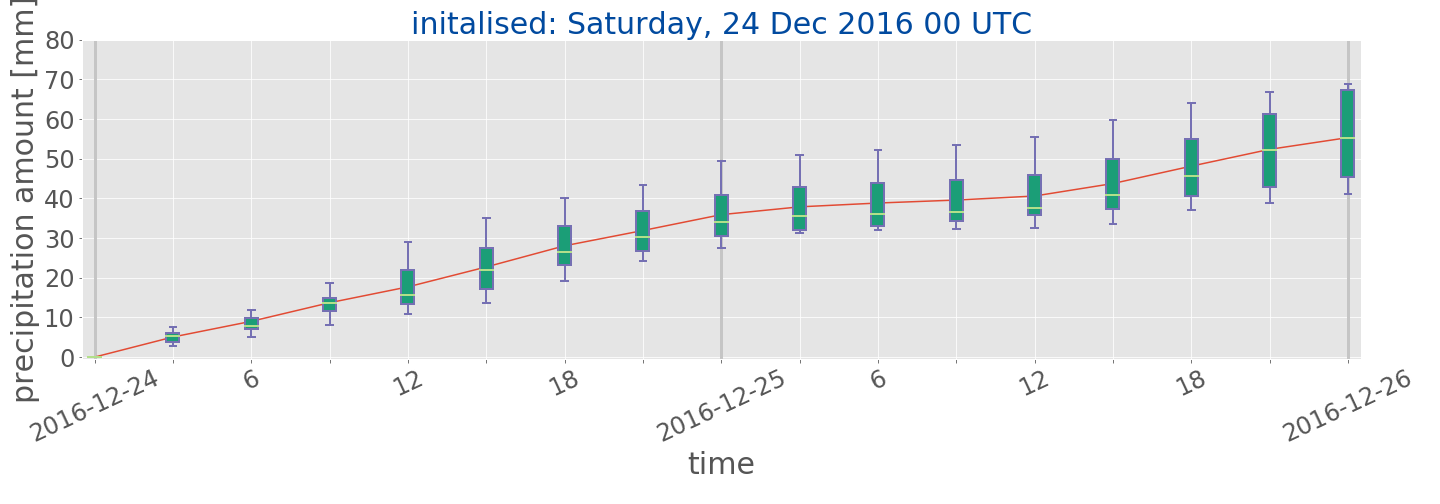
\includegraphics[trim ={0cm 2.2cm 0cm 0cm},clip,width=\textwidth]{./fig_boxplot_sfc/20161224_0}
		\caption{}\label{fig:boxplot:24}
	\end{subfigure}
	%
	\begin{subfigure}[b]{\textwidth}
		\centering
		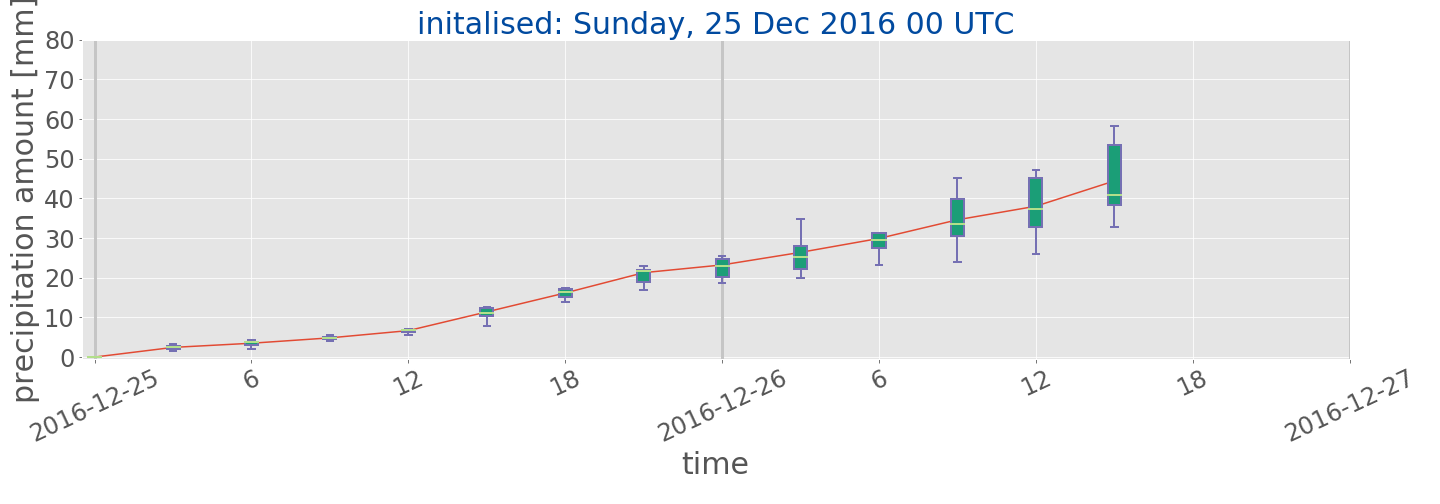
\includegraphics[trim ={0cm 2.2cm 0cm 0cm},clip,width=\textwidth]{./fig_boxplot_sfc/20161225_0}
		\caption{}\label{fig:boxplot:25}
	\end{subfigure}
	%
	\begin{subfigure}[b]{\textwidth}
		\centering
		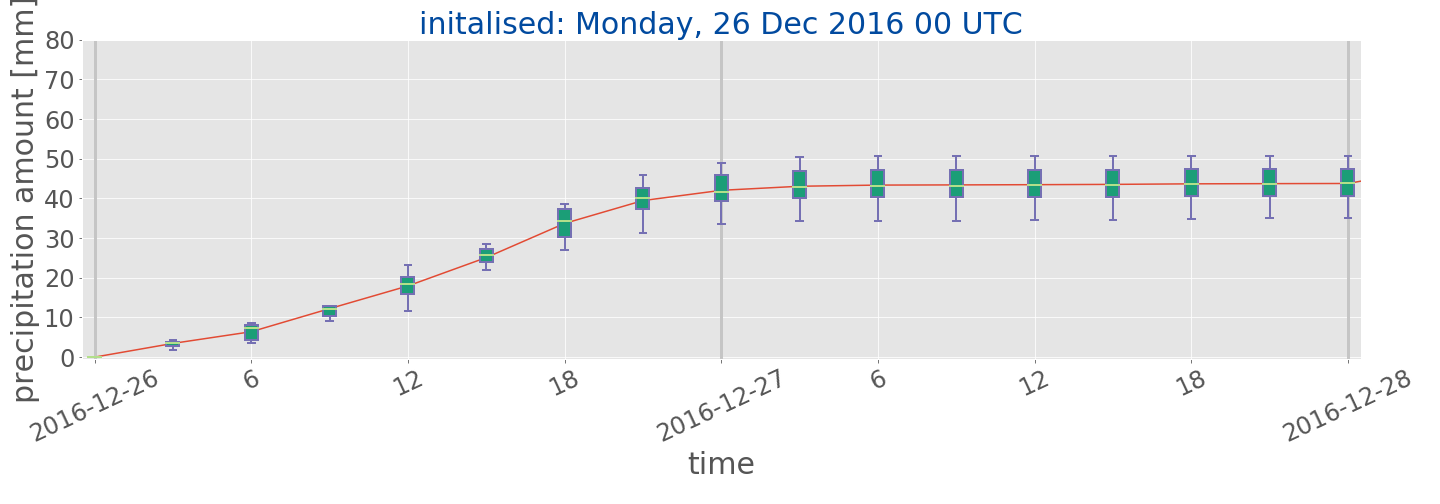
\includegraphics[trim ={0cm 1.cm 0cm 0cm},clip,width=\textwidth]{./fig_boxplot_sfc/20161226_0}
		\caption{}\label{fig:boxplot:26}
	\end{subfigure}
	\caption{Box-whisker-plot of the ten ensemble members of MEPS. Red line indicating the ensemble mean, lower and upper whisker the 25th and 75th percentile, respectively. Light green shows the median of all members and the box represents the middle \SI{50}{\percent} of scores of the precipitation.}\label{fig:boxplot}
\end{figure}
%%%%%%%%%%%%%%%%%%%%%%%%%%%%%%%%%%%%%%%%%%%%%%%%%%%%%%%%%%%%%%%%%%%%%%%%%%
\noindent
The box-whisker-plot in \Cref{fig:boxplot} displays the distribution of the ten ensemble members for the respective days. All three days with overestimation seem to have different variability. As expected increases the forecast uncertainty with longer forecast time for precipitation amount.  
\\
%On \SI{25}{\dec}, the least variability between the ten ensemble members of up to almost \SI{24}{\hour} is shown in \Cref{fig:boxplot:25}. 
The variability in \Cref{fig:ens_vari} show on \SI{25}{\dec} no large variation between the ensemble members (narrow box-whiskers). This day is also the forecast with the smallest wet bias of the three days with overestimation (\Cref{fig:bias:precip12}. More variation between the ensemble members is shown on \num{24} and \SI{26}{\dec} after \SI{3}{\hour}.
As the correlation for precipitation amount in \Cref{fig:scat:precip2426} suggests, the overestimation is not as high as for \num{24} and \SI{26}{\dec}. On \num{24} and \SI{25}{\dec} the mean error for the surface accumulation is largest with values up to \SI{7}{\mm} for \SI{12}{\hour} (\Cref{fig:MAE:precip12}. 
\\
Larger variability is already present after \SI{3}{\hour} prediction time in \Cref{fig:boxplot:24} on \SI{24}{\dec}. The spread between the ensemble members (shown by the minimum and maximum whiskers) seems to be wide indicating a larger uncertainty about the amount of surface accumulation. The ensemble mean (red line) is always higher than the median, suggesting a positively skewed distribution. After \SI{12}{\hour} forecast time, the median is closer to the lower 25th percentile, indicating a negative skewness. Also, all upper whiskers in \Cref{fig:boxplot:24} are longer than the lower ones, which would follow that the ensemble members vary amongst the most positive quartile and that it is very similar for the least positive quartile group. 
%Since the deterministic forecast, black line in \Cref{fig:sfc_acc24}, is in the upper percentile compared to its perturbed members it follows that for this forecast the deterministic forecast was not the best guess for the surface accumulation and by using the 'wrong' initial state it can have led to larger miscalculations. 
\\
I believe that the uncertainty appearing already after \SI{3}{\hour} (\Cref{fig:boxplot:24}) could be associated with a too long spin-up time of MEPS. MEPS usually has a spin-up time of about three hours, on \SI{24}{\dec} this might have been longer as a result of poorer initial conditions \textcolor{red}{Need a reference here, not stated in \citet{muller_arome-metcoop:_2017}}. 
%The regional model MEPS receives initial and boundary conditions from ECMWF before it can produce forecasts \citep{muller_arome-metcoop:_2017}. Since initial conditions such as observations have uncertainties as well as the model has mistrust, and  the own climatology needs to be approached, a model has to stabilize before the simulations can be trusted. The spin-up time varies depending on the quality of the initial and boundary conditions. 
It seems, that the initial and boundary conditions for MEPS might have not been perfect for initialisations on \SI{24}{\dec} at \SI{0}{\UTC}. As described in \Cref{sec:DIM:MEPS} should the perturbed members always lie relatively close to the observations. For a short time (hours) should the forecast member be close together \citep{kalnay_atmospheric_2003}. 
The deterministic and perturbed members might not to have stabilised yet and show larger variation in \Cref{fig:boxplot:24} from early on than e.g. on \SI{25}{\dec}. More variability between the ensemble members do not necessarily mean, that a forecast is bad, it only shows the uncertainty of the initial conditions. Important is, that the observations, which are going to be used for the initialisation are within the spread of the ensemble member prediction.
\\
The uncertainty might also have been related to the fact that the large-scale situation got more complex. The precipitation amount associated with the transition of an occluded front on \SI{23}{\dec}, after \SI{18}{\UTC}, is higher than on the previous days (\Cref{fig:res:sfc_precip23} and \Cref{fig:TPU}). During \num{20} to \SI{21}{\dec}, the hourly precipitation around \SI{0}{\UTC} is less intense than on \SI{23}{\dec} (\Cref{fig:TPU23}). High accumulation amount over shorter time followed and could have resulted in a larger variability of the MEPS members (\Cref{fig:boxplot}). Another possibility is MEPS might have accounted for additional accumulation around \SI{12}{\UTC} on \SI{24}{\dec} and this showed a stronger increase in accretion in \Cref{fig:sfc_acc24} at \SI{13}{\UTC}. I believe it could be associated to a local resolution effect of MEPS at Haukeliseter, which will be further discussed in \Cref{sec:res:oro_infl}. 
\\
\\
\Cref{fig:boxplot:25} and \subref{fig:boxplot:26} show a smaller ensemble member variability on \SIlist{25;26}{\dec} than on \SI{24}{\dec}. The box-whiskers are narrower for the first \SI{30}{\hour} in \Cref{fig:boxplot:25}, but slightly larger after \SI{6}{\hour} forecast time for initialisations on \SI{26}{\dec}. \Cref{sec:res:large_scale_sfc} presented a good agreement between observations and forecast of large scale features in terms of pressure, temperature and wind direction. While the occlusion on \SI{26}{\dec} was more intuitive (\Cref{fig:res:sfc_pres26,fig:res:sfc_temp26,fig:res:sfc_wd26,fig:res:sfc_ws26}) than the warm front development on \SI{25}{\dec} (\Cref{fig:res:sfc_pres25}, \subref{fig:res:sfc_temp25}, \subref{fig:res:sfc_wd25}, \subref{fig:res:sfc_ws25}). The mean error in \Cref{fig:bias} for each variable shows to be best on \SI{25}{\dec} (\Cref{fig:MAE:pres},\subref{fig:MAE:temp},\subref{fig:MAE:wd}, \subref{fig:MAE:ws}, and \subref{fig:MAE:precip12}).
\\
On \SI{25}{\dec} the overestimation started to occur around \SI{13}{\UTC} in \Cref{fig:sfc_acc25}, and may be related to the delayed temperature MEPS forecasted temperature increase in \Cref{fig:res:sfc_temp25}.  As \Cref{fig:boxplot:25} shows, the variability in the forecast increases after \SI{15}{\hour} prediction time. In general, median and mean agree well for the entire period of a \SI{48}{\hour} lead time. After \SI{39}{\hour} the mean is much higher than the median and closer to the lower 25th percentile in \Cref{fig:boxplot:25}. It seems, that all ten ensemble members agree well on the prediction and nevertheless MEPS overestimates the surface accumulation. The MEPS surface forecasts on \SI{25}{\dec} suggest that MEPS did not expect the occurrence of a warm front (\Cref{fig:res:sfc_pres25,fig:res:sfc_temp25,fig:res:sfc_wd25,fig:res:sfc_ws25}). However, the surface accumulation prediction could suggest that MEPS expected more precipitation around \SI{12}{\UTC}. Maybe MEPS has expected a weak warm-front passage and therefore more precipitation. The fact that the temperature is rising and therefore the phase is changing from snow to liquid precipitation (\Cref{fig:res:obs_masc}) may have led to MEPS expecting more liquid precipitation rather than mixed phase precipitation and hence MEPS predicted more surface accumulation.
%I consider that MEPS misinterpreted the amount of precipitation related to the transition of the warm sector.  
\\
Between \SIlist{15;18}{\UTC} on \SI{26}{\dec}, the core of the low-pressure system passes over Haukeliseter \Cref{fig:res:sfc_pres26,fig:res:sfc_temp26,fig:res:sfc_wd26,fig:res:sfc_ws26}. The box-whiskers in \Cref{fig:boxplot:26} indicate a larger variability after \SI{6}{\hour} prediction while the precipitation amount forecast is overestimating at \SI{12}{\UTC}. The forecast precipitation amount is similar to the double fence observations, but overestimated.
%and following the structure of the double fence observation. 
Variability of all ensemble members increases at \SI{6}{\hour} lead time, but then decreases again in \Cref{fig:boxplot:26}.  
\\
Since the box-whisker-plot in \Cref{fig:boxplot:25} and \subref{fig:boxplot:26} (\num{25} and \SI{26}{\dec}) show less variability in the beginning it is assumed that spin-up time issues are less likely, but not totally excluded. It could be related to an error in the initialisation state, even though it does not show within the variability at the beginning. 
%An error associated with the spin-up time of MEPS is not totally excluded for these days. 
In \Cref{fig:sfc_acc25} and \subref{fig:sfc_acc26}, the ensemble mean agrees well with the deterministic forecast, which is an indication of a symmetrical spread around the deterministic run. Again, the ensemble mean is the best statistical solution over a longer timespan and does not necessarily mean to be the best for an extreme event such as the Christmas storm 2016. 
\\ 
The overestimation of accumulated precipitation during \num{24} and \SI{26}{\dec} might be related 
%to the high forecasted wind speeds, 
local topography as well as to the complex development of the low-pressure system north-west of Norway on \SI{24}{\dec}. Furthermore could it be related to the \SI{10}{\percent} under-catchment by the double fence gauge under high wind condition.
\\
\\
According to \citet{muller_arome-metcoop:_2017} strong precipitation events are better predicted with AROME-MetCoOp than with ECMWF. In \Cref{sec:dim:dec_obs} it was described, that during \num{21} to \SI{27}{\dec} \SI{56.9}{\percent} of the total December 2016 accumulation of precipitation were observed. 
%\citet{muller_arome-metcoop:_2017} states also, that an overestimation appears, where the precipitation event (\SI{12}{\hour} accumulation) is less than \SI{10}{\mm} this seems not to be true for all days but could be possible for \num{25} and \SI{26}{\dec} (observed accumulation in \Cref{tab:sfc_acc}). 
In December 2014, the \SI{12}{\hour} precipitation mean absolute error in AROME-MetCoOp was below \SI{1.5}{\mm} \citep{muller_arome-metcoop:_2017}. For the 2016 Christmas storm the mean absolute error is not larger than \SI{5}{\mm} for the first \SI{12}{\hour} of accumulation on \num{24} and \SI{26}{\dec}
(\Cref{fig:MAE:precip12}). Therefore, the assumption follows that on \SI{26}{\dec} the overestimation might be correlated to the <\SI{10}{\mm} problem described by \citet{muller_arome-metcoop:_2017}. The \SIlist{12;24}{\hour} accumulation is presented in \Cref{tab:res:MEPS_err} for Haukeliseter and shows that \SI{12}{\hour} observed accretion was less than \SI{10}{\mm} for 
\num{25} and \SI{26}{\dec}.
%On \SI{25}{\dec} the mean absolute error was \SI{1.1}{\mm} for the first \SI{12}{\hour} accumulation and shows that this could be an influence but does not necessarily mean to be the case, because the general mean absolute error is small (\Cref{fig:MAE:precip}). 
The mean error for \SI{12}{\hour} accumulation in fact shows a wet bias during \num{24} and \SI{26}{\dec}.
%since the overestimation started to occur after \SI{11}{\hour} prediction time. 
%%%%%%%%%%%%%%%%%%%%%%%%%%%%%%%%%%%%%%%%%%%%%%%%%%%%%%%%%%%%%%%%%%%%%%%%%%


%%%%%%%% large scale phenomena vertical ? %%%%%%%%%%%%%%
\subsection{Comparison of snow water content in the vertical}%\label{sec:res:verticalSWC}
\label{sec:res:large_scale_vert}
%%%%%%%%% image reflectivity %%%%%%%%%%%%%%
\begin{figure}[h!]
	\centering
	% 23/12
	\begin{subfigure}[t]{\textwidth}
		\centering
		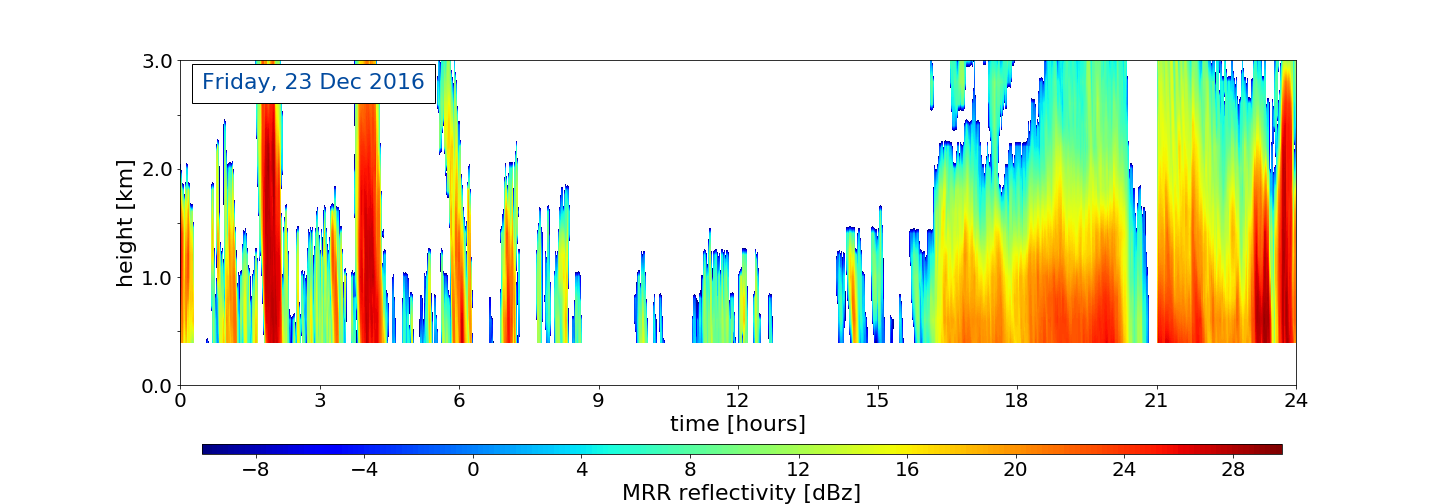
\includegraphics[trim={4.cm 2.5cm 4.5cm 1.5cm},clip,width=0.9\textwidth]{./fig_MRR_refl/MRR_20161223}
		\caption{}\label{fig:ret:refl23}
	\end{subfigure}
	% 25/12
	\begin{subfigure}[t]{\textwidth}
		\centering
		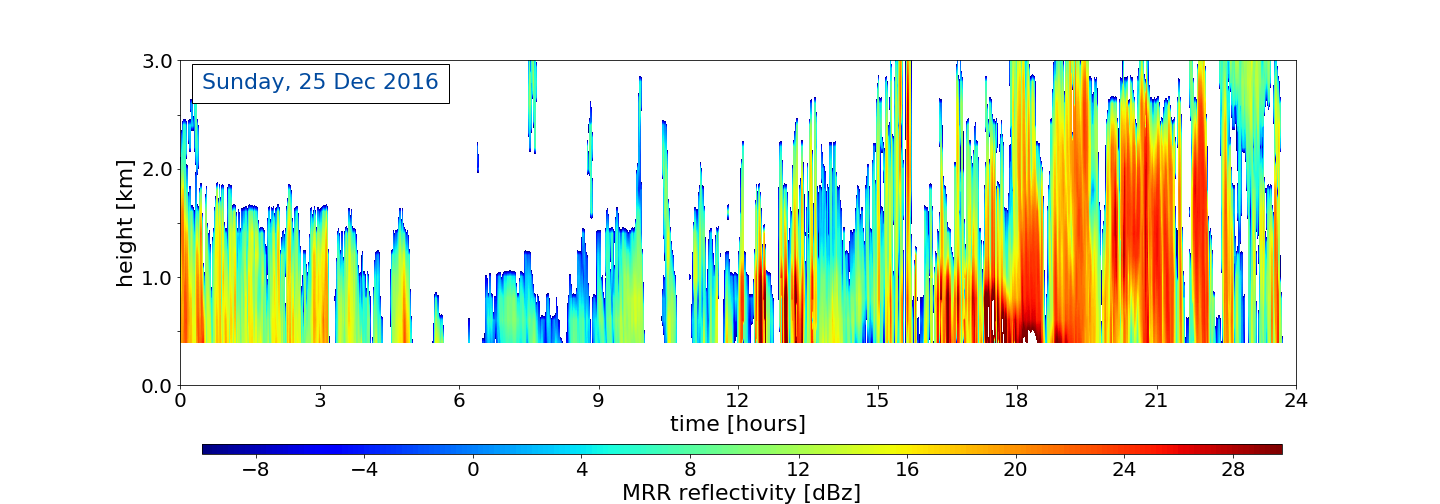
\includegraphics[trim={4.cm 2.5cm 4.5cm 1.5cm},clip,width=0.9\textwidth]{./fig_MRR_refl/MRR_20161225}
		\caption{}\label{fig:ret:refl25}
	\end{subfigure}
	% 26/12
	\begin{subfigure}[t]{\textwidth}
		\centering
		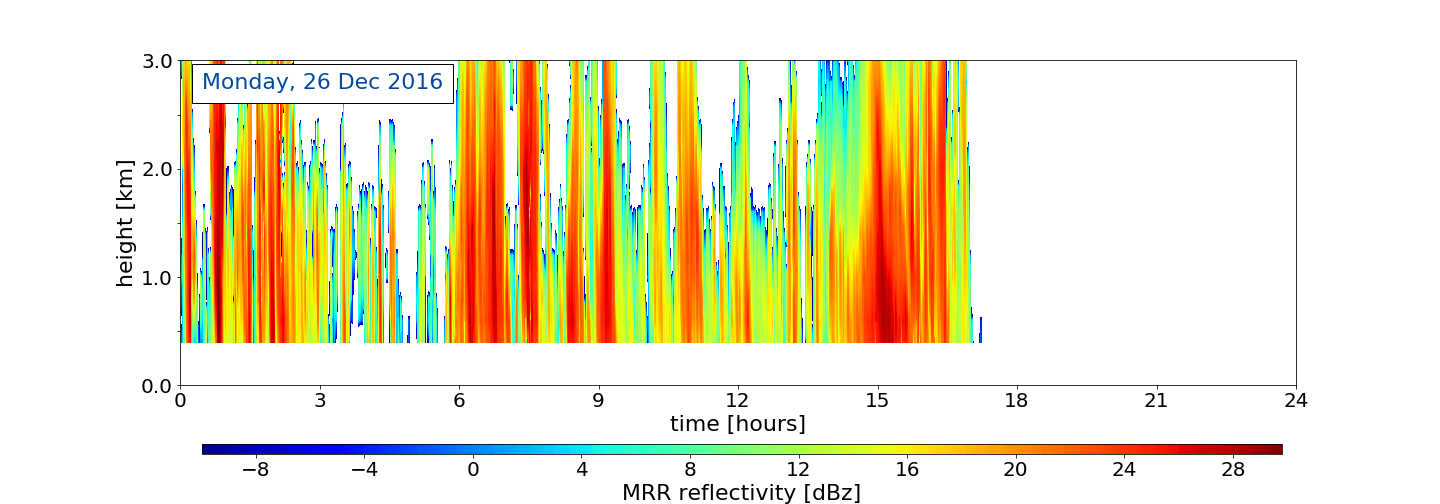
\includegraphics[trim={4.cm 2.5cm 4.5cm 1.5cm},clip,width=0.9\textwidth]{./fig_MRR_refl/MRR_20161226}
		\caption{}\label{fig:ret:refl26}
	\end{subfigure}
	% label
	\begin{subfigure}[t]{\textwidth}
		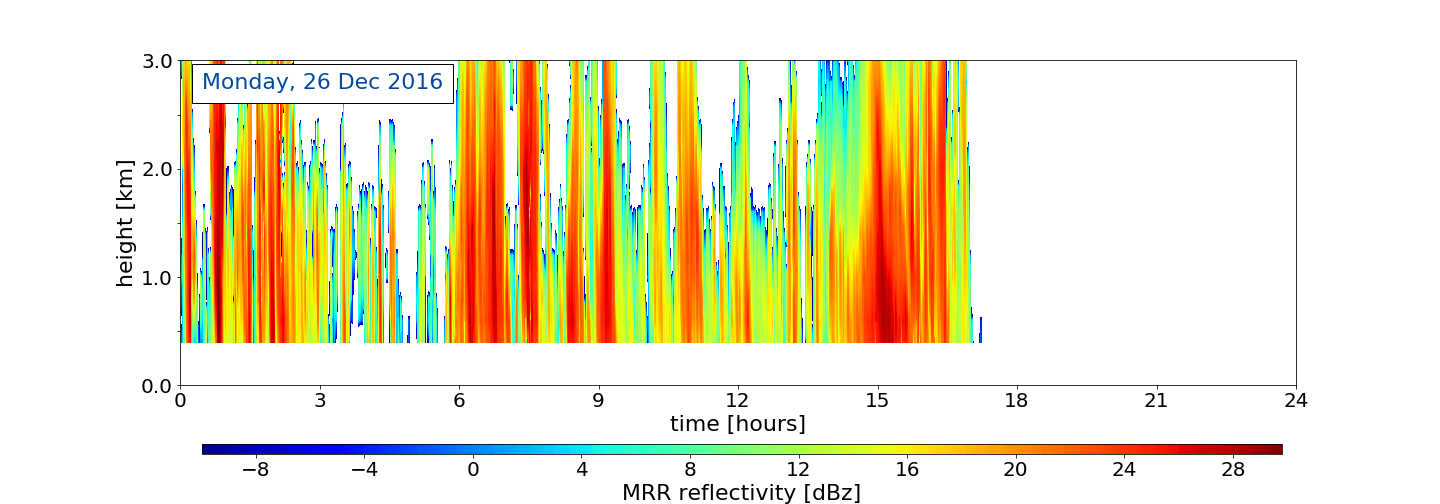
\includegraphics[trim={6.5cm 0cm 5.3cm 15.5cm},clip,width=\textwidth]{./fig_MRR_refl/MRR_20161226}
	\end{subfigure}
	\caption{MRR reflectivity for the days when a front or an occlusion passed through at Haukeliseter. \SI{}{\decibel Z} reflectivity according to the colour bar, with weaker precipitation in blue and more intense precipitation in red. \protect\subref{fig:ret:refl23}: Friday, \SI{23}{\dec}, \protect\subref{fig:ret:refl25}: Sunday, \SI{25}{\dec}, and \protect\subref{fig:ret:refl26}: Monday, \SI{26}{\dec}.}\label{fig:ret:refl}
\end{figure}
%%%%%%%%%%%%%%%%%%%%%%%%%%%%%%%%%%%%%%%%%%%%%%%%%%%%%%%%%%%%%%%%%%%%%%%%%
\noindent
Frontal boundary passages were observed at the surface several times throughout the extreme storm in December 2016. MEPS is able to predict the large scale features and related surface changes for initialisation more than \SI{24}{\hour} before (\Cref{sec:res:large_scale_sfc}). In winter 2016 three additional instruments were installed to estimate the vertical snow water content at Haukeliseter. This unique approach gives the opportunity to compare the vertical forecasts of SWC to vertical solid precipitation observations. 
%As far as the author knows is there no study on this particular topic about the verification of vertical ensemble member prediction models with observations.
\\
Previous studies such as \citet{joos_influence_2012} motivate to make accurate surface measurements more available to improve mesoscale models.
\\
Passages of occluded fronts and a warm sector were observed on \num{23}, \num{26}, and \SI{25}{\dec}, respectively.
\Cref{fig:ret:refl} shows the reflectivity from the MRR at Haukeliseter for these three days. \Cref{fig:ret:refl26} presents only values until \SI{17}{\UTC}, because of the temperature change and hence a precipitation shift followed liquid drops freezing on the MRR dish and the signal got attenuated. 
\\
More consistent storm structure with higher reflectivity values indicat the transition of the boundaries in \Cref{fig:ret:refl}.
%The transit of the boundaries is shown in \Cref{fig:ret:refl} by more consistent structure of a storm with higher reflectivity values. 
While on \num{23} and \SI{26}{\dec} the reflectivity did not pass values larger than \SI{28}{\decibel Z} shows \Cref{fig:ret:refl25} high reflectivity values larger than \SI{30}{\decibel Z} (compare for approximation \Cref{tab:ref_values}). These high values indicate the observation of possible liquid precipitation. Images from the MASC were able to verify observed liquid drops during \SIrange{12}{21}{\UTC} (\Cref{fig:res:obs_masc}). 
\\
On \SI{23}{\dec}, the surface observations allow to assume that the occluded front passed through between \SIrange{12}{21}{\UTC} (\Cref{fig:res:sfc_pres23}, \subref{fig:res:sfc_temp23}, \subref{fig:res:sfc_wd23}). The vertical observations at Haukeliseter show intense reflectivity and therefore more intense precipitation after \SI{16}{\UTC} (\Cref{fig:ret:refl23}). Another occlusion passed through on \SI{26}{\dec} shortly before \SI{15}{\UTC} which lasted until \SI{21}{\UTC} indicated by a more consistent storm structure and high reflectivity in \Cref{fig:ret:refl26} around \SI{15}{\UTC}. The high reflectivity on both days shows the passage of the occlusion and the associated precipitation. On \SI{23}{\dec}, the wind is from the south, upslope (\Cref{fig:res:sfc_wd23}, \Cref{fig:site:kartverket}) which led to a more consistent storm structure in \Cref{fig:ret:refl23}. \Cref{fig:res:sfc_wd25} and \subref{fig:res:sfc_ws25} indicate strong wind observations from the west which led to a consistent, but shorter storm structure in \Cref{fig:ret:refl25} at \SI{15}{\UTC} on \SI{25}{\dec}. The orographic influenced wind and therefore a possible relation to the precipitation will be further assessed in \Cref{sec:res:oro_infl}. 
\\
\\
\Cref{fig:ret:SWC} presents the reflectivity of the MRR and the snow water content retrieved from the reflectivity as well as the \SI{48}{\hour} forecast values. Minutely MRR reflectivity and retrieved snow water content can be seen in \Cref{fig:SWC:ret_22}, \subref{fig:SWC:ret_23}, \subref{fig:SWC:ret_25}, and \subref{fig:SWC:ret_26}. \Cref{fig:SWC_EM:22}, \subref{fig:SWC_EM:23}, \subref{fig:SWC_EM:25}, \subref{fig:SWC_EM:26} show in the upper panel the hourly averaged values from the retrieved SWC and in the lower panel the ensemble mean of the instantaneous forecast values every hour over all ensemble member.   
Three hourly averaged retrieved values are then presented in the upper panel of \Cref{fig:SWC3h:22}, \subref{fig:SWC3h:23}, \subref{fig:SWC3h:25}, and \subref{fig:SWC3h:26}, the lower panel are the ensemble mean forecast values every three hours.
\\
\Cref{fig:SWC_EM:23} (lower panel) shows the one hourly averaged forecast values over all ensemble members, neglecting not existing values on \SI{23}{\dec}. 
%Initialisations less than \SI{24}{\hour} before the event predict the consistent retrieved snowfall after \SI{16}{\UTC} (\Cref{fig:SWC:ret_23}, lower panel and \Cref{fig:SWC_EM:23}, upper panel). 
Forecasts initialised \SI{48}{\hour} (\SI{22}{\dec}) prior predict the consistent storm structure and therefore the passage of the front (\Cref{fig:SWC_EM:22}, \subref{fig:SWC3h:22}). 
The consistent structure of retrieved snowfall after \SI{16}{\UTC} is predicted for initialisations less than \SI{24}{\hour} before the occurrence of the occlusion (\Cref{fig:SWC:ret_23}, \subref{fig:SWC_EM:23}, and \subref{fig:SWC3h:23}).
Even the three hourly resolved averaged forecast values show a response on the occurrence of the storm (\Cref{fig:SWC3h:23}, lower panel). 
The duration of the passage is between \SIrange{16}{23}{\UTC} (\Cref{fig:SWC:ret_22} to \subref{fig:SWC3h:23}). MEPS is able to estimate the snow water content for time resolutions of \SI{3}{\hour} in \Cref{fig:SWC3h:22}, \subref{fig:SWC3h:23}.
%%%%%%%%% image SWC retrieval MEPS 22 %%%%%%%%%%%%%%
\begin{figure}[H]
	\centering
	% 23/12
	\begin{subfigure}[t]{\textwidth}
		\centering
		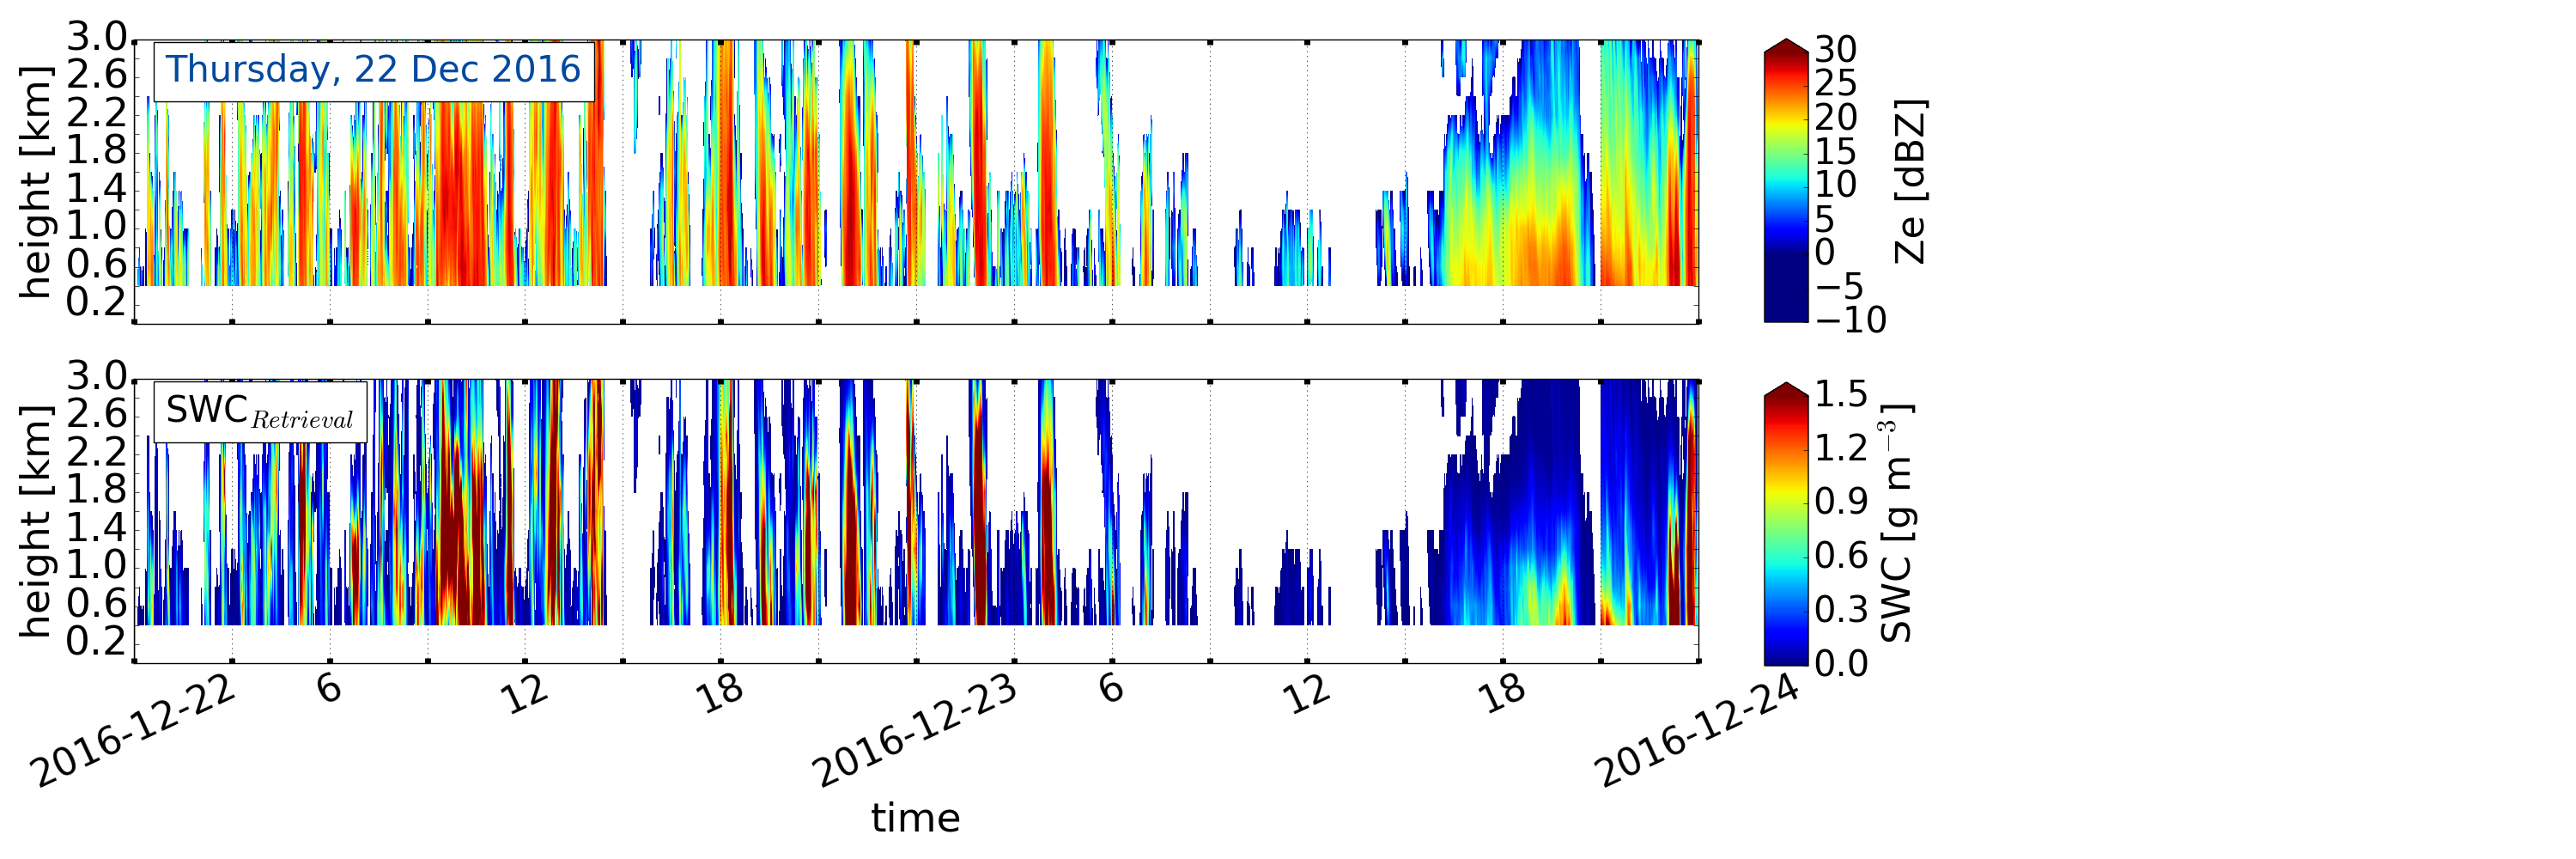
\includegraphics[trim={0.cm 2.2cm 19.cm 0.5cm},clip,width=0.9\textwidth]{./fig_obs_ret/20161222}
		\caption{}\label{fig:SWC:ret_22}
	\end{subfigure}
	% EM
	\begin{subfigure}[t]{\textwidth}
		\centering
		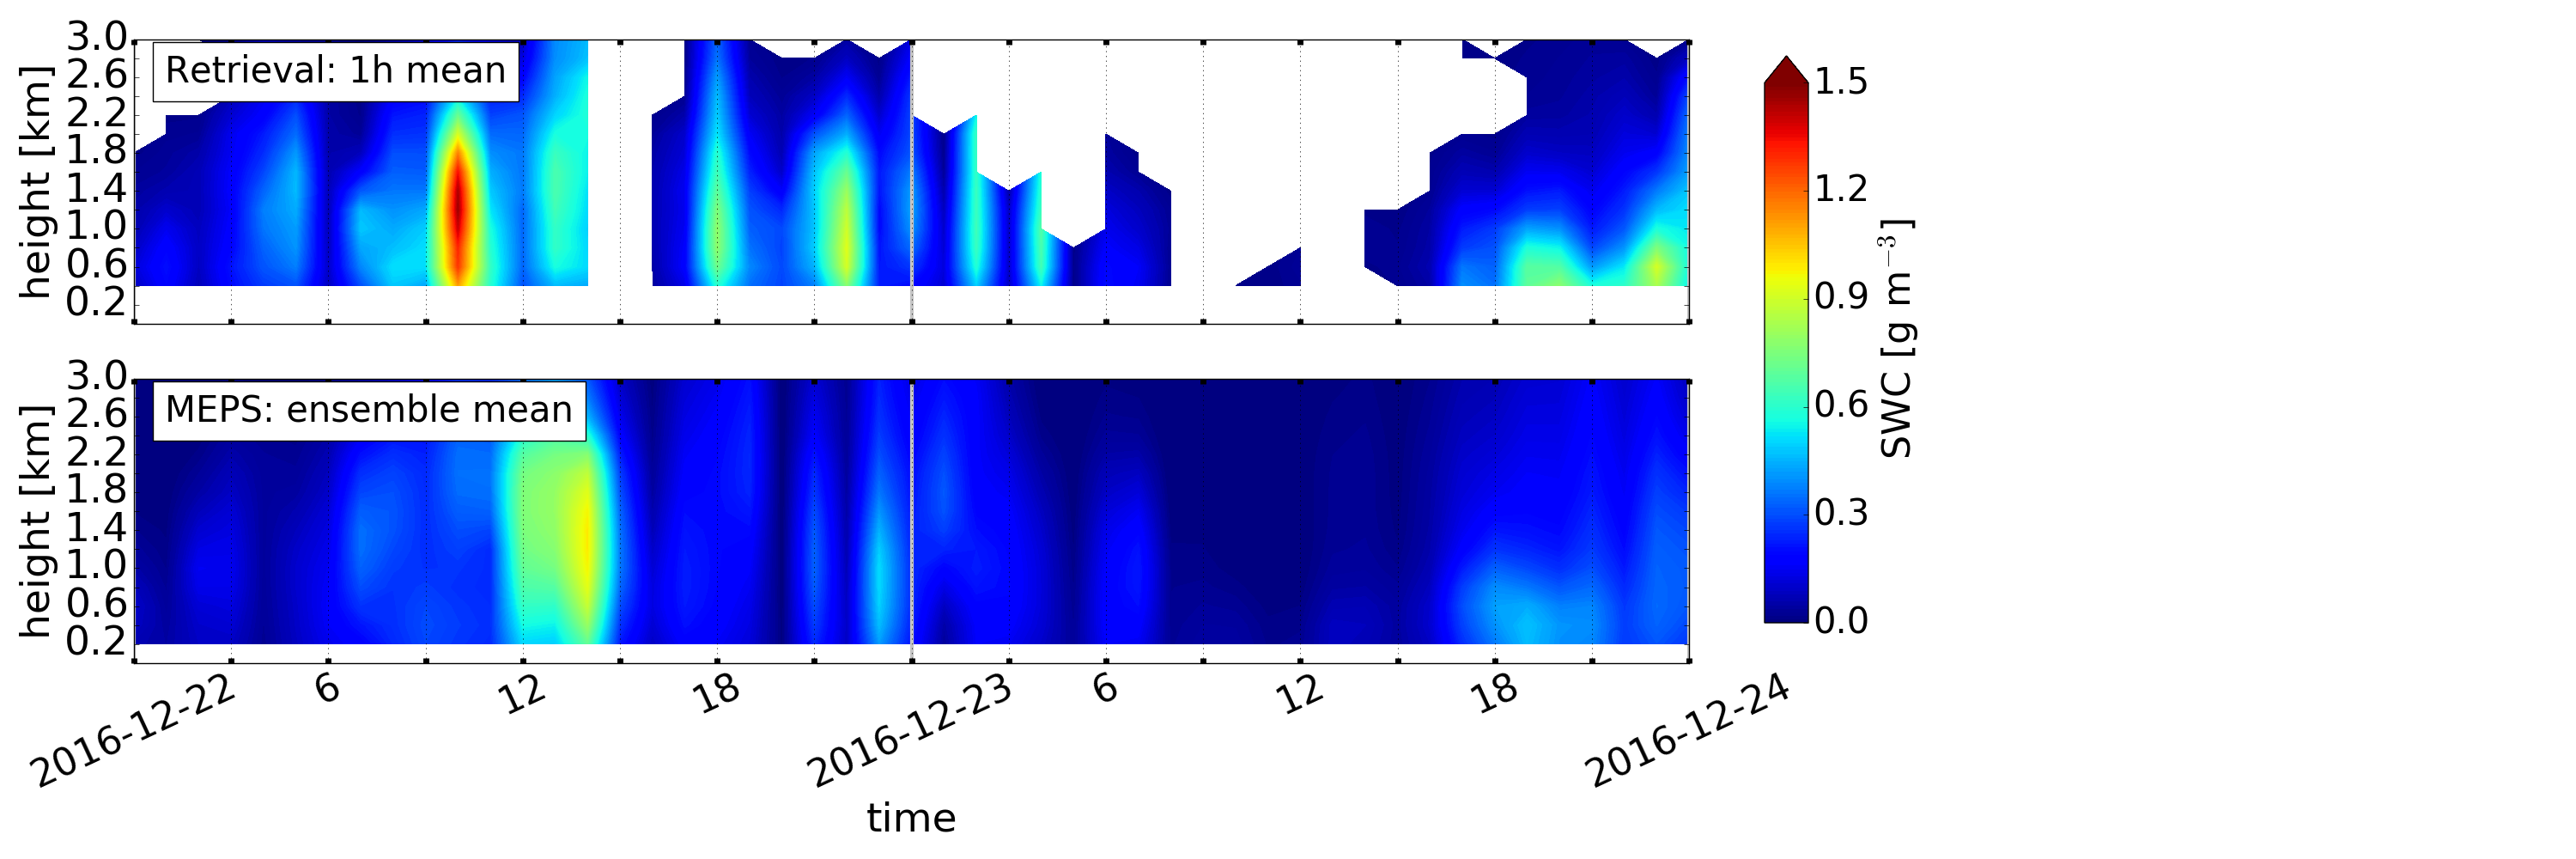
\includegraphics[trim={0.cm 2.2cm 19.cm 0.5cm},clip,width=0.9\textwidth]{./fig_vert_SWC_EM/20161222}
		\caption{}\label{fig:SWC_EM:22}
	\end{subfigure}
	% 3h
	\begin{subfigure}[t]{\textwidth}
		\centering
		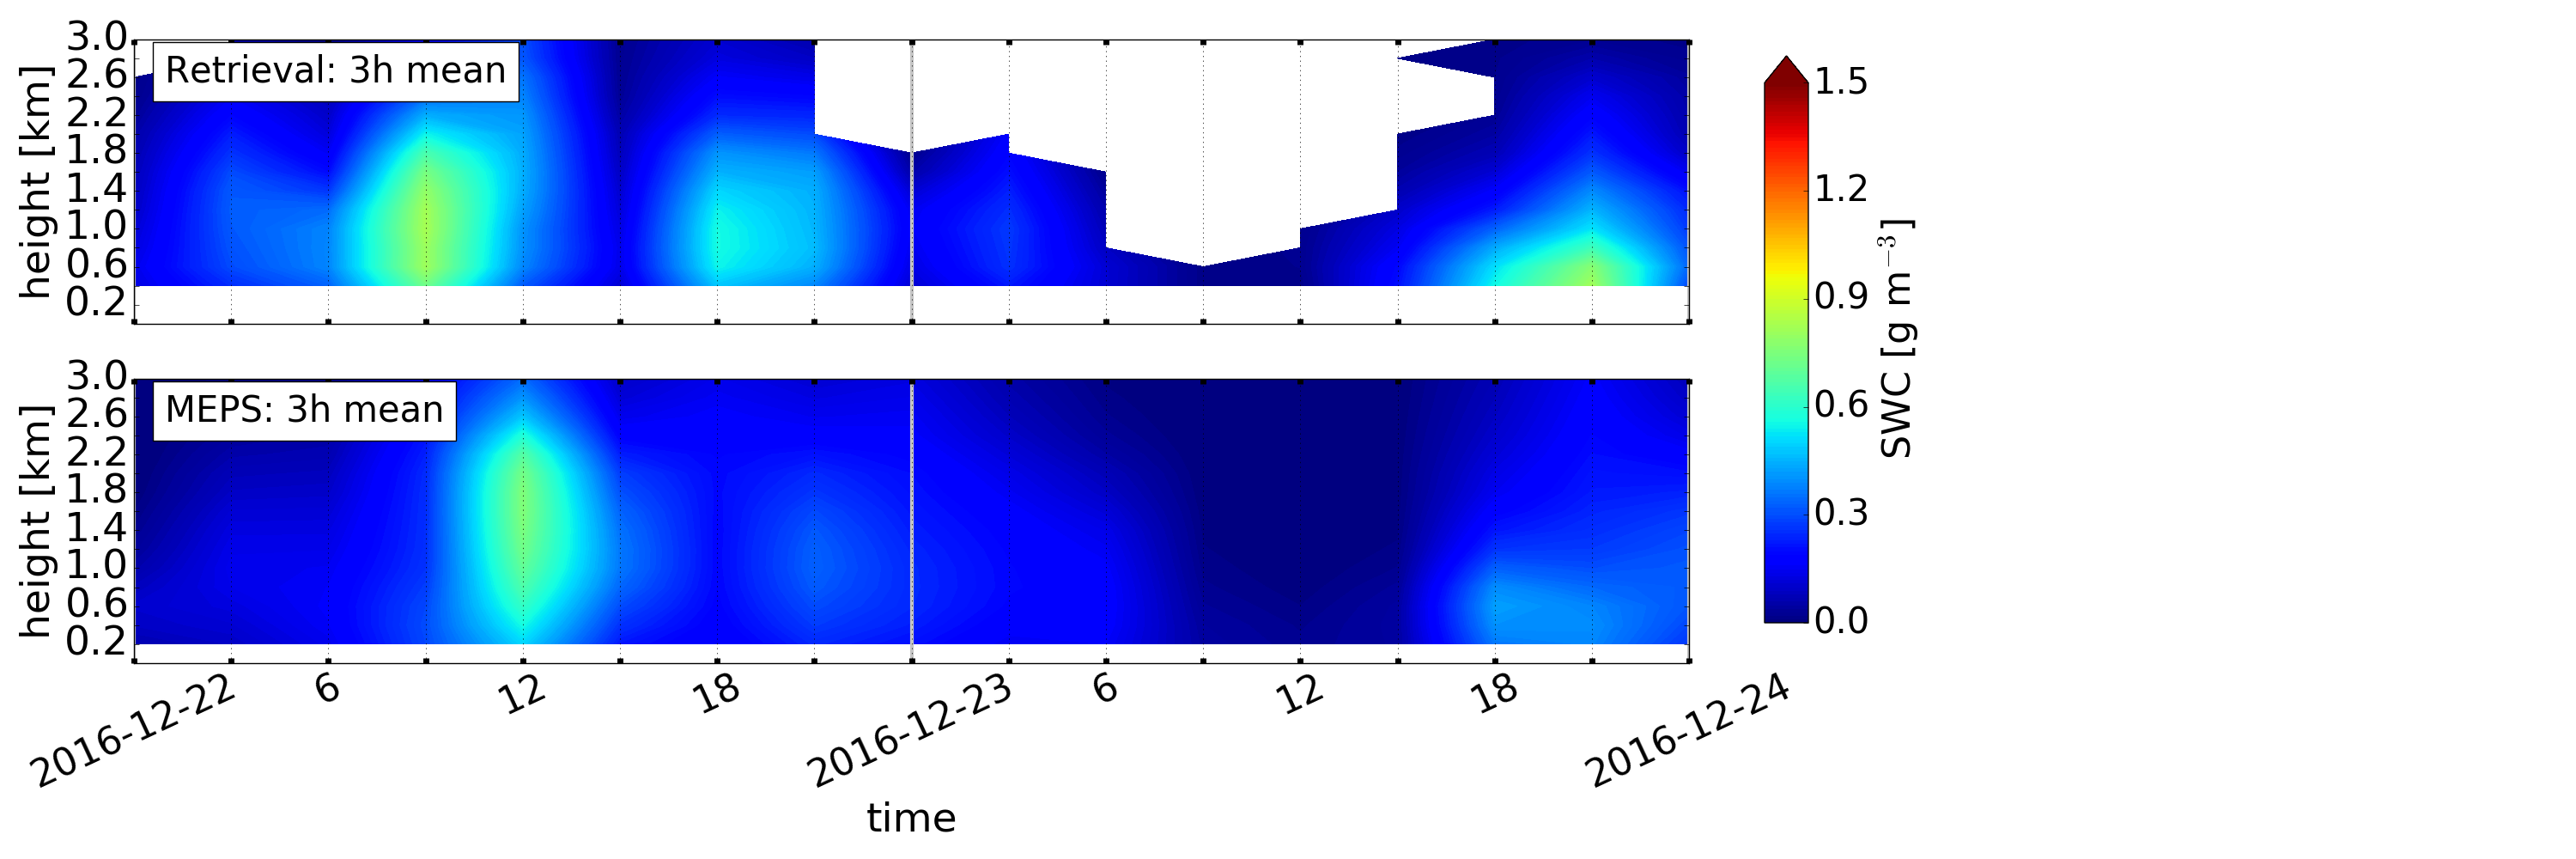
\includegraphics[trim={0.cm 0.8cm 19.cm 0.5cm},clip,width=0.9\textwidth]{./fig_vert_SWC_3h/20161222}
		\caption{}\label{fig:SWC3h:22}
	\end{subfigure}
	\caption{Initialisation on \SI{22}{\dec} %\SIlist{22;23;25;24;26}{\dec} 
		at \SI{0}{\UTC}. From top to bottom: (\protect\subref{fig:SWC:ret_22}) MRR reflectivity for \SI{48}{\hour}, minutely retrieved SWC.
		%, \protect\subref{fig:SWC:ret_23}, \protect\subref{fig:SWC:ret_24}, \protect\subref{fig:SWC:ret_25}, \protect\subref{fig:SWC:ret_26})  
		(\protect\subref{fig:SWC_EM:22}) Hourly averaged retrieved SWC, lower panel instantaneous hourly averaged forecast of all ensemble member SWC, neglecting missing values.  
		%   (\protect\subref{fig:SWC_EM:22}, \protect\subref{fig:SWC_EM:23}, \protect\subref{fig:SWC_EM:24}, \protect\subref{fig:SWC_EM:25}, \protect\subref{fig:SWC_EM:26}) Upper panel: hourly averaged retrieved SWC, lower panel instantaneous hourly averaged forecast of all ensemble member SWC, neglecting missing values. 
		(\protect\subref{fig:SWC3h:22}) Three hourly averaged retrieved SWC, lower panel instantaneous three hourly averaged forecast of all ensemble member SWC.%, \protect\subref{fig:SWC3h:23}, \protect\subref{fig:SWC3h:24}, \protect\subref{fig:SWC3h:25}, \protect\subref{fig:SWC3h:26}) Upper panel three hourly averaged retrieved SWC, lower panel instantaneous three hourly averaged forecast of all ensemble member SWC. 
		\textit{Continued on next page.}  }\label{fig:ret:SWC}
\end{figure}
%%%%%%%%% image SWC retrieval MEPS 23 %%%%%%%%%%%%%%
\begin{figure}[H]\ContinuedFloat
	\centering
	% 23/12
	\begin{subfigure}[t]{\textwidth}
		\centering
		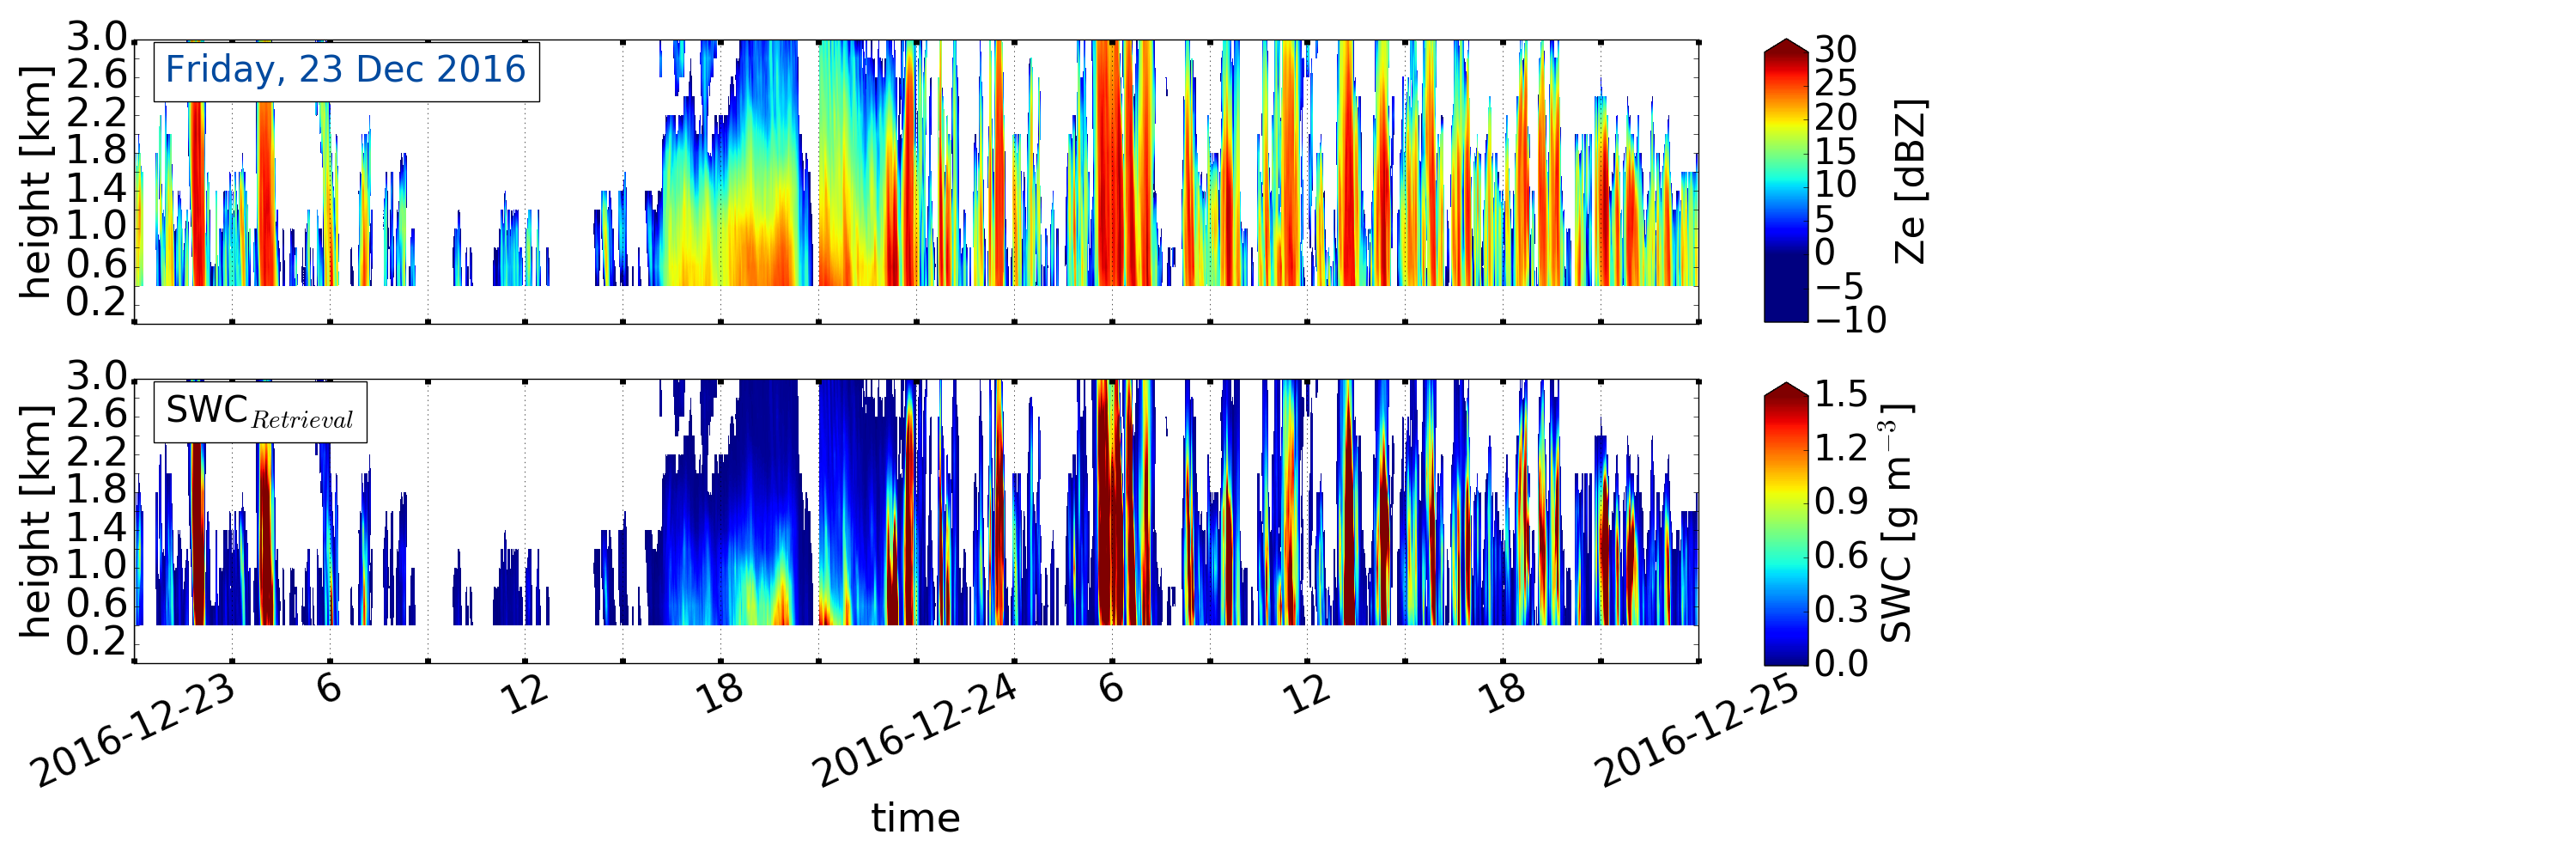
\includegraphics[trim={0.cm 2.2cm 19.cm 0.5cm},clip,width=0.9\textwidth]{./fig_obs_ret/20161223}
		\caption{}\label{fig:SWC:ret_23}
	\end{subfigure}
	% EM
	\begin{subfigure}[t]{\textwidth}
		\centering
		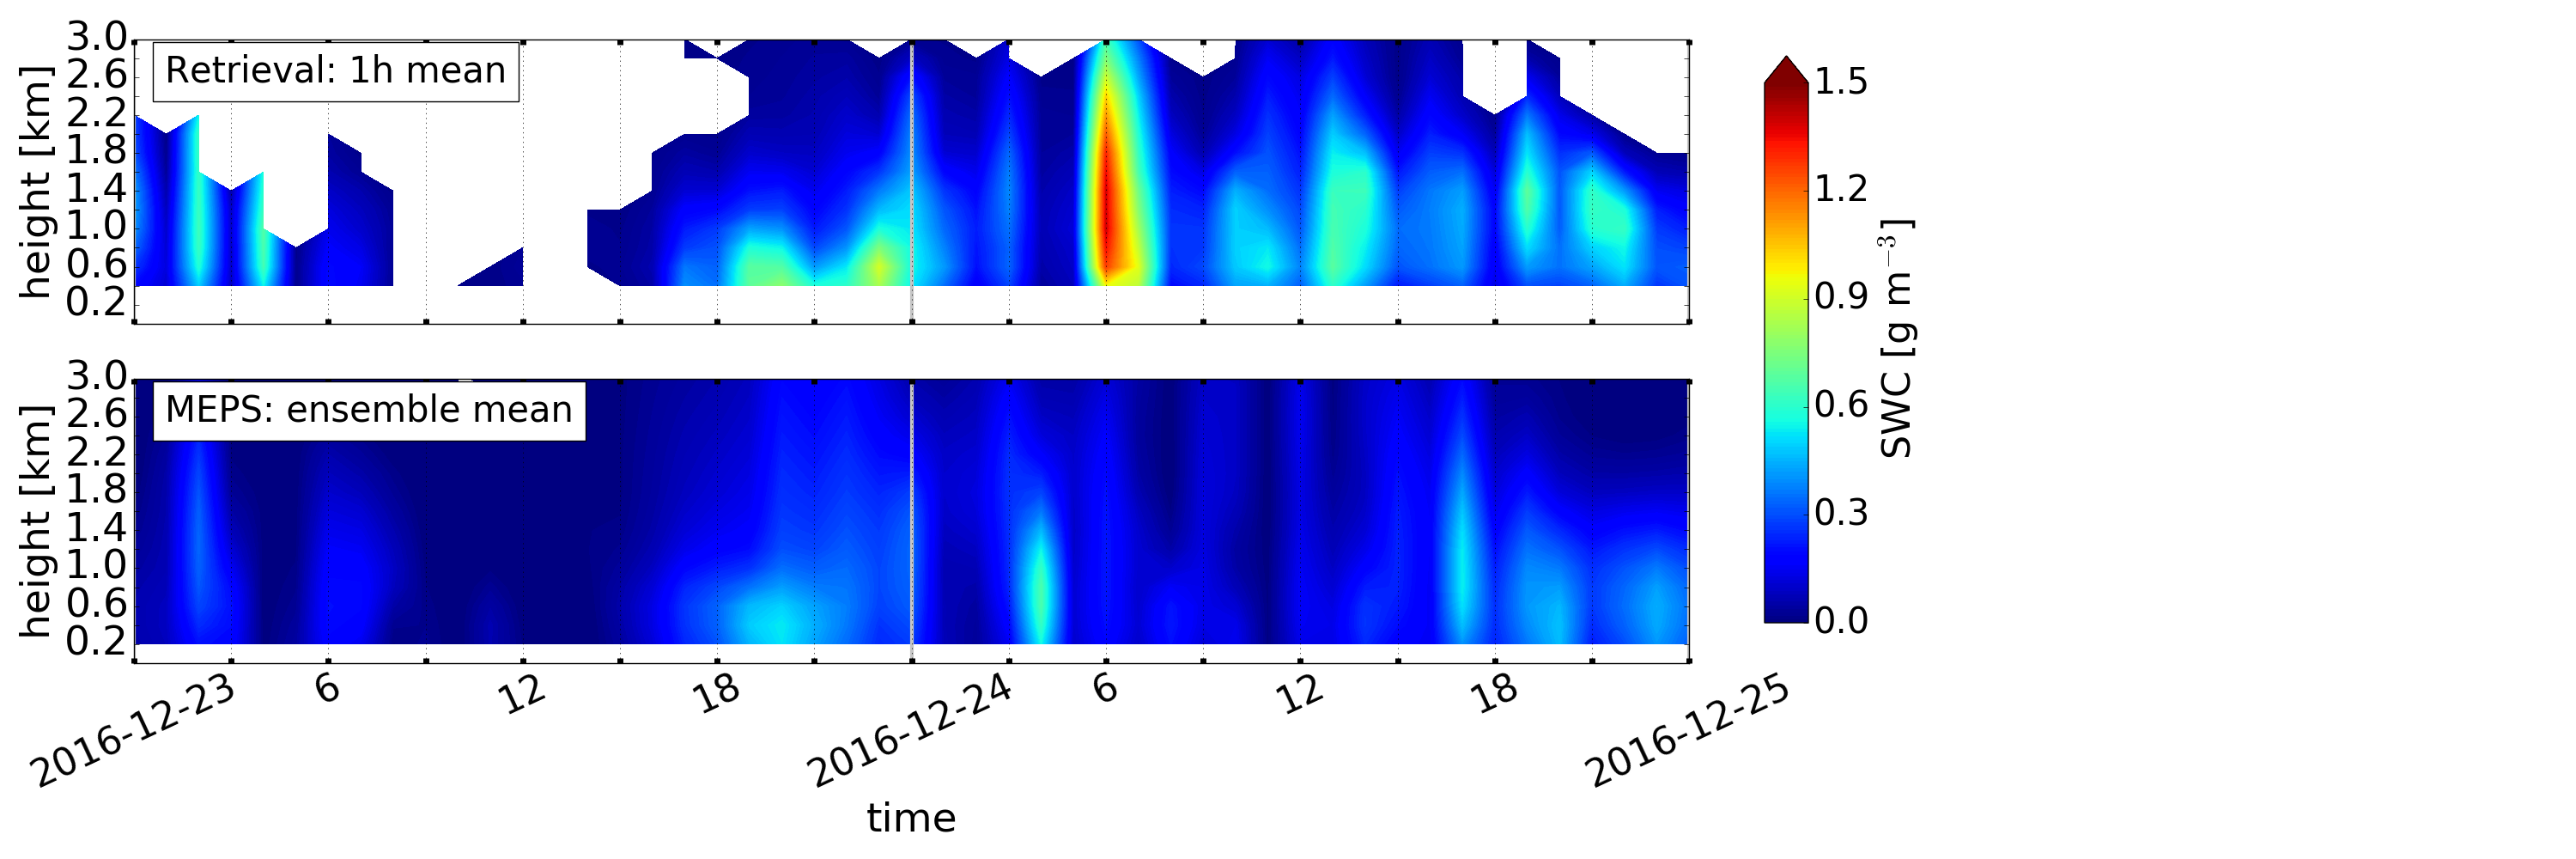
\includegraphics[trim={0.cm 2.2cm 19.cm 0.5cm},clip,width=0.9\textwidth]{./fig_vert_SWC_EM/20161223}
		\caption{}\label{fig:SWC_EM:23}
	\end{subfigure}
	% 3h
	\begin{subfigure}[t]{\textwidth}
		\centering
		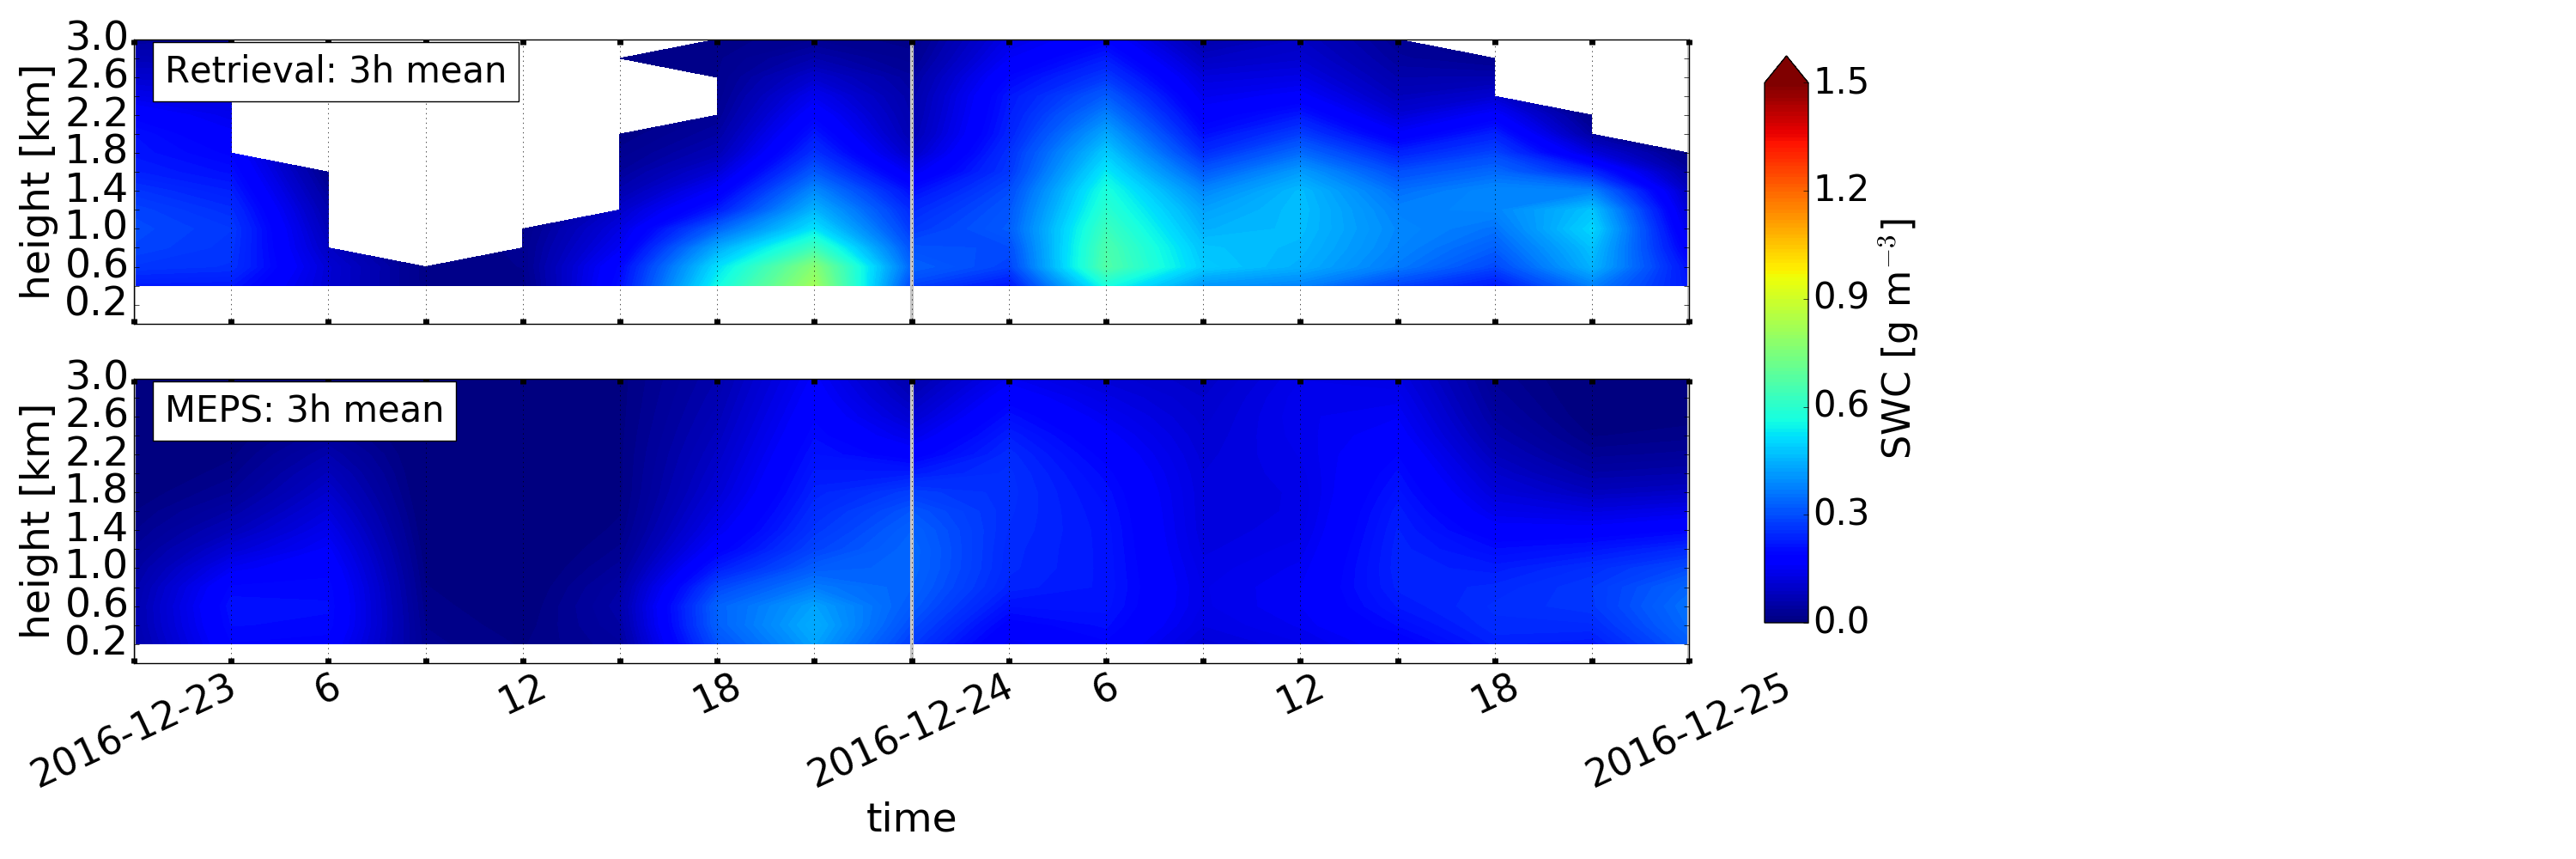
\includegraphics[trim={0.cm 0.8cm 19.cm 0.5cm},clip,width=0.9\textwidth]{./fig_vert_SWC_3h/20161223}
		\caption{}\label{fig:SWC3h:23}
	\end{subfigure}
	\caption{\textit{(Continued from previous page.)} Initialisation \SI{23}{\dec} at \SI{0}{\UTC}.}
\end{figure}
%%%%%%%%% image SWC retrieval MEPS 24 %%%%%%%%%%%%%%
\begin{figure}[H]\ContinuedFloat
	\centering
	% 24/12
	\begin{subfigure}[t]{\textwidth}
		\centering
		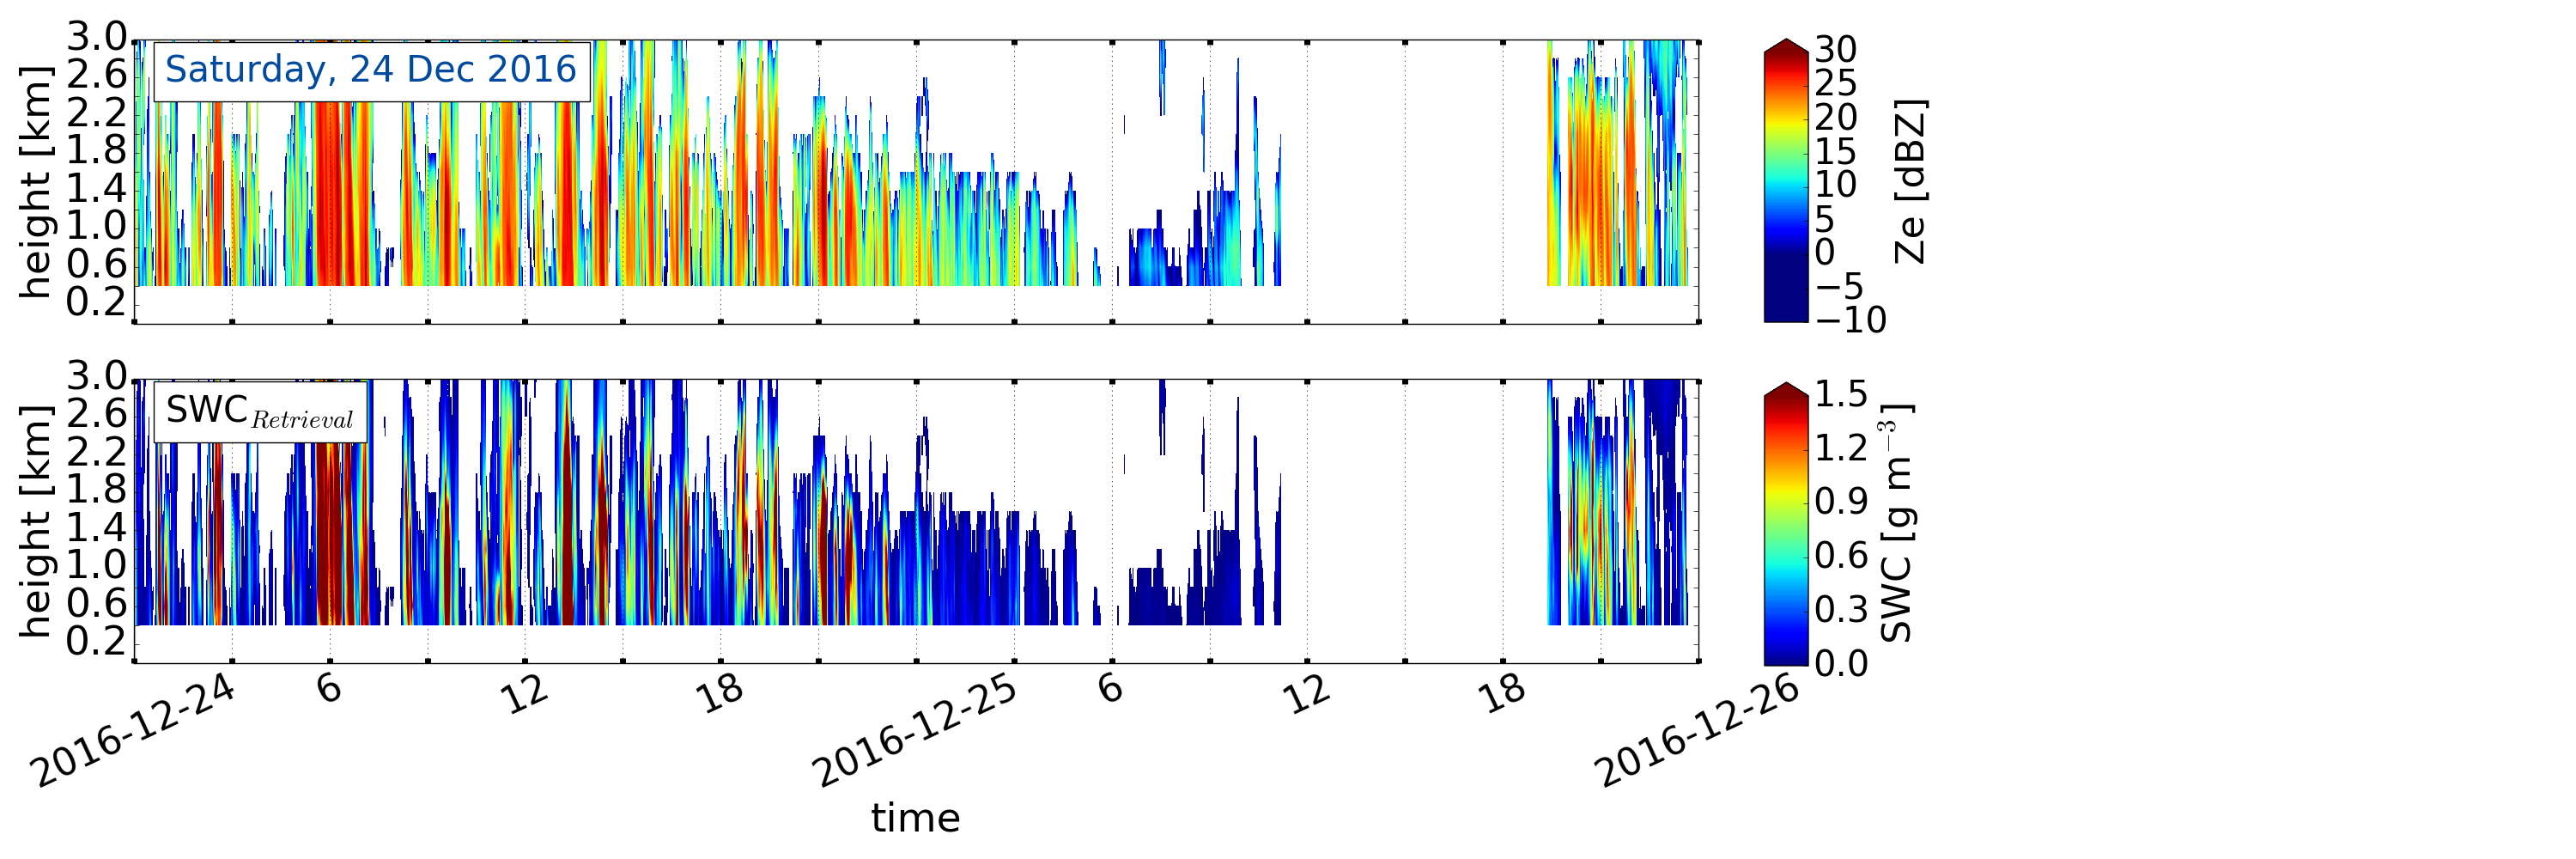
\includegraphics[trim={0.cm 2.2cm 19.cm 0.5cm},clip,width=0.9\textwidth]{./fig_obs_ret/20161224}
		\caption{}\label{fig:SWC:ret_24}
	\end{subfigure}
	% EM
	\begin{subfigure}[t]{\textwidth}
		\centering
		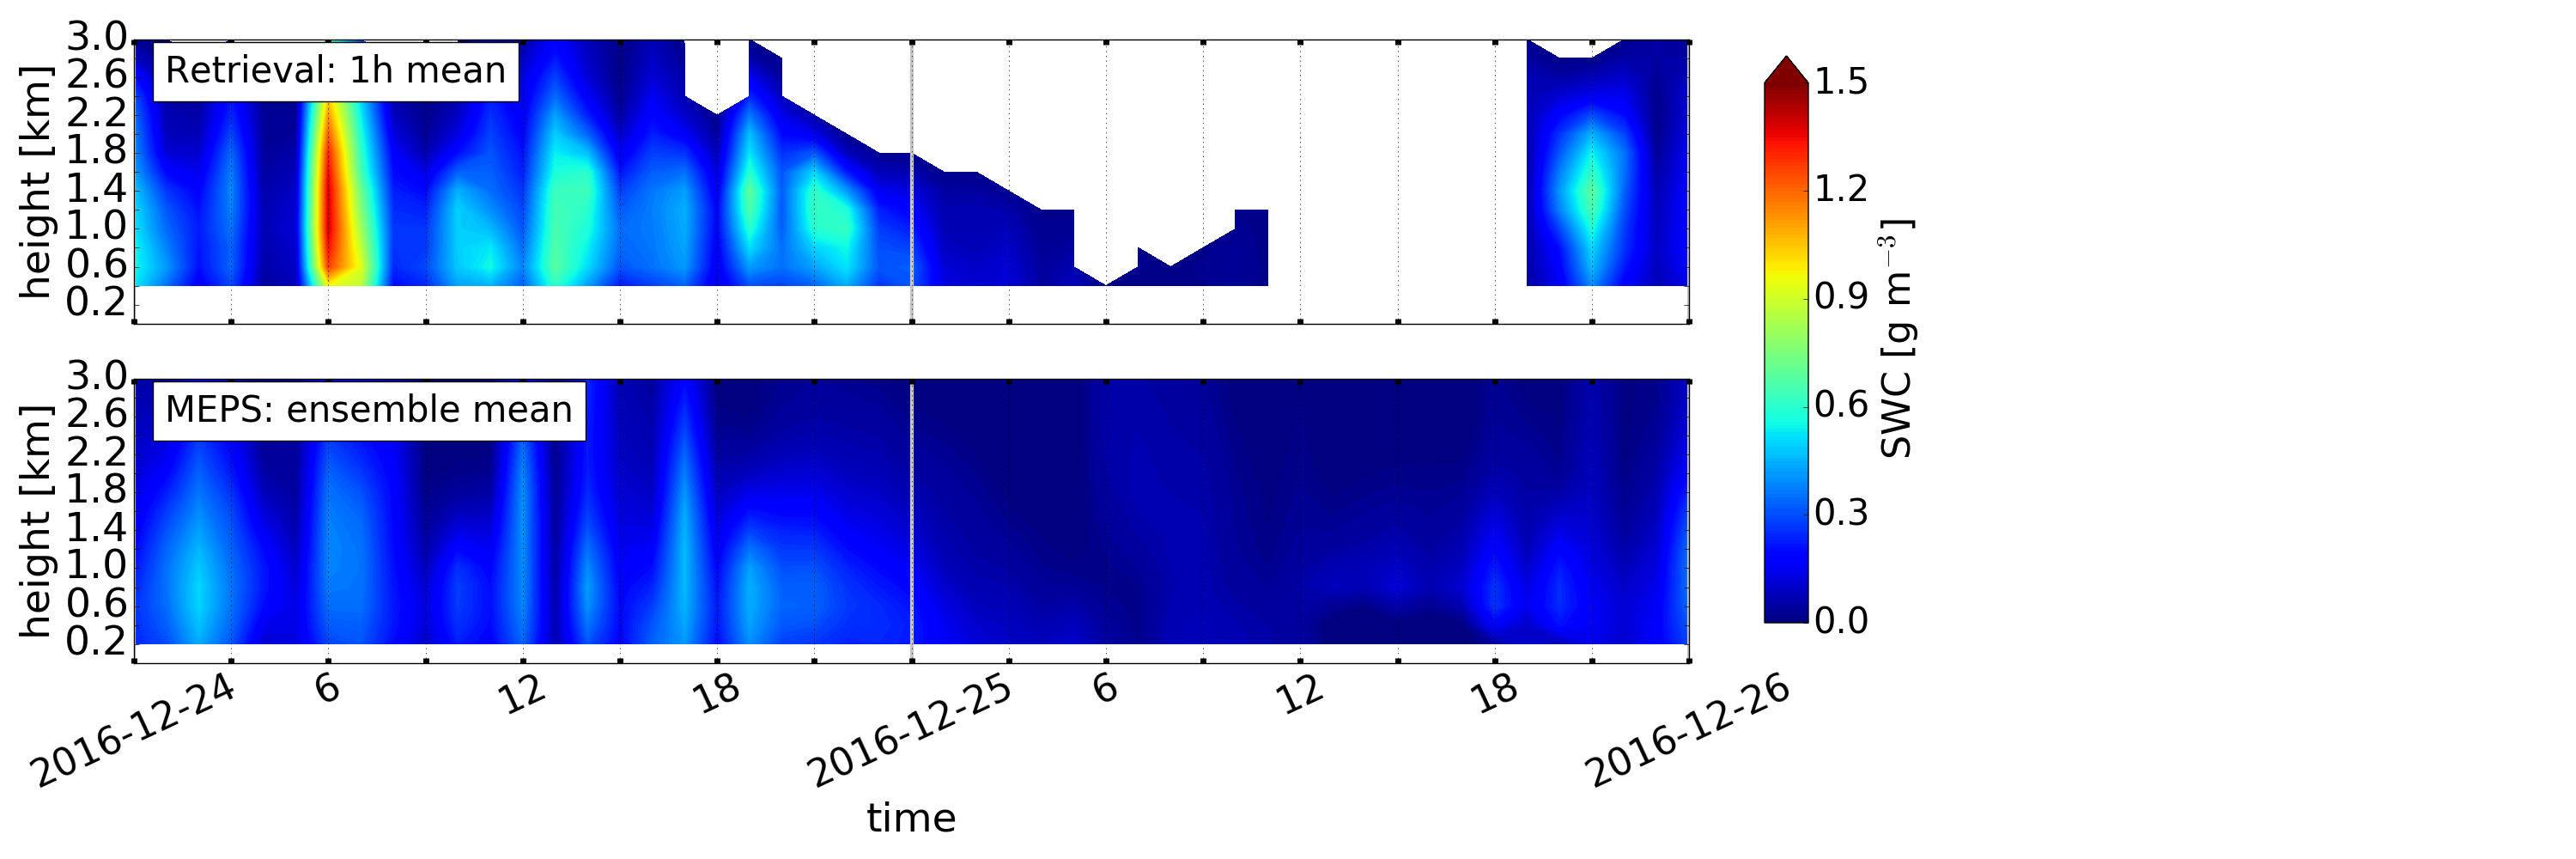
\includegraphics[trim={0.cm 2.2cm 19.cm 0.5cm},clip,width=0.9\textwidth]{./fig_vert_SWC_EM/20161224}
		\caption{}\label{fig:SWC_EM:24}
	\end{subfigure}
	% 3h
	\begin{subfigure}[t]{\textwidth}
		\centering
		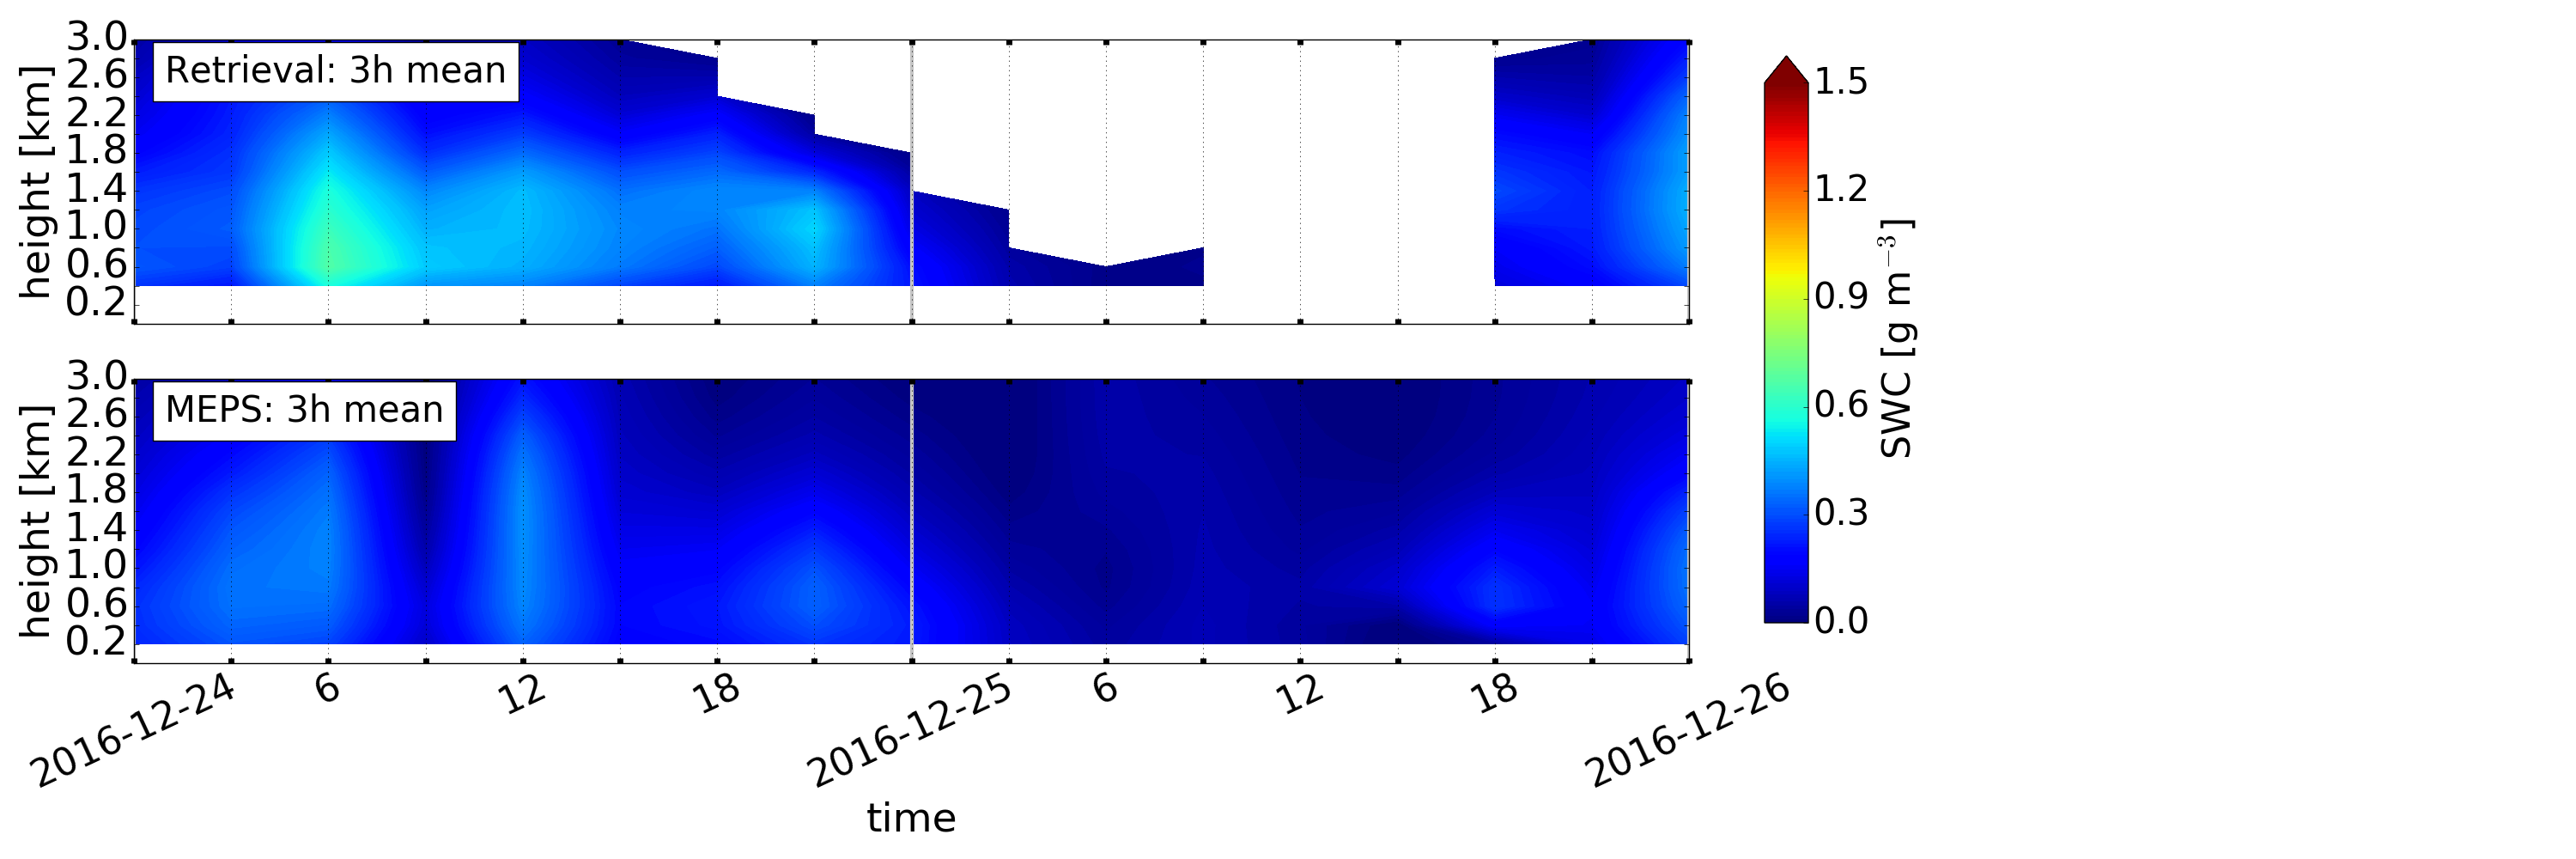
\includegraphics[trim={0.cm 0.8cm 19.cm 0.5cm},clip,width=0.9\textwidth]{./fig_vert_SWC_3h/20161224}
		\caption{}\label{fig:SWC3h:24}
	\end{subfigure}
	\caption{\textit{(Continued from previous page.)} Initialisation \SI{26}{\dec} at \SI{0}{\UTC}.}
\end{figure}
%%%%%%%%%%%%%%%%%%%%%%%%%%%%%%%%%%%%%%%%%%%%%%
%%%%%%%%% image SWC retrieval MEPS 25 %%%%%%%%%%%%%%
\begin{figure}[H]\ContinuedFloat
	\centering
	% 25/12
	\begin{subfigure}[t]{\textwidth}
		\centering
		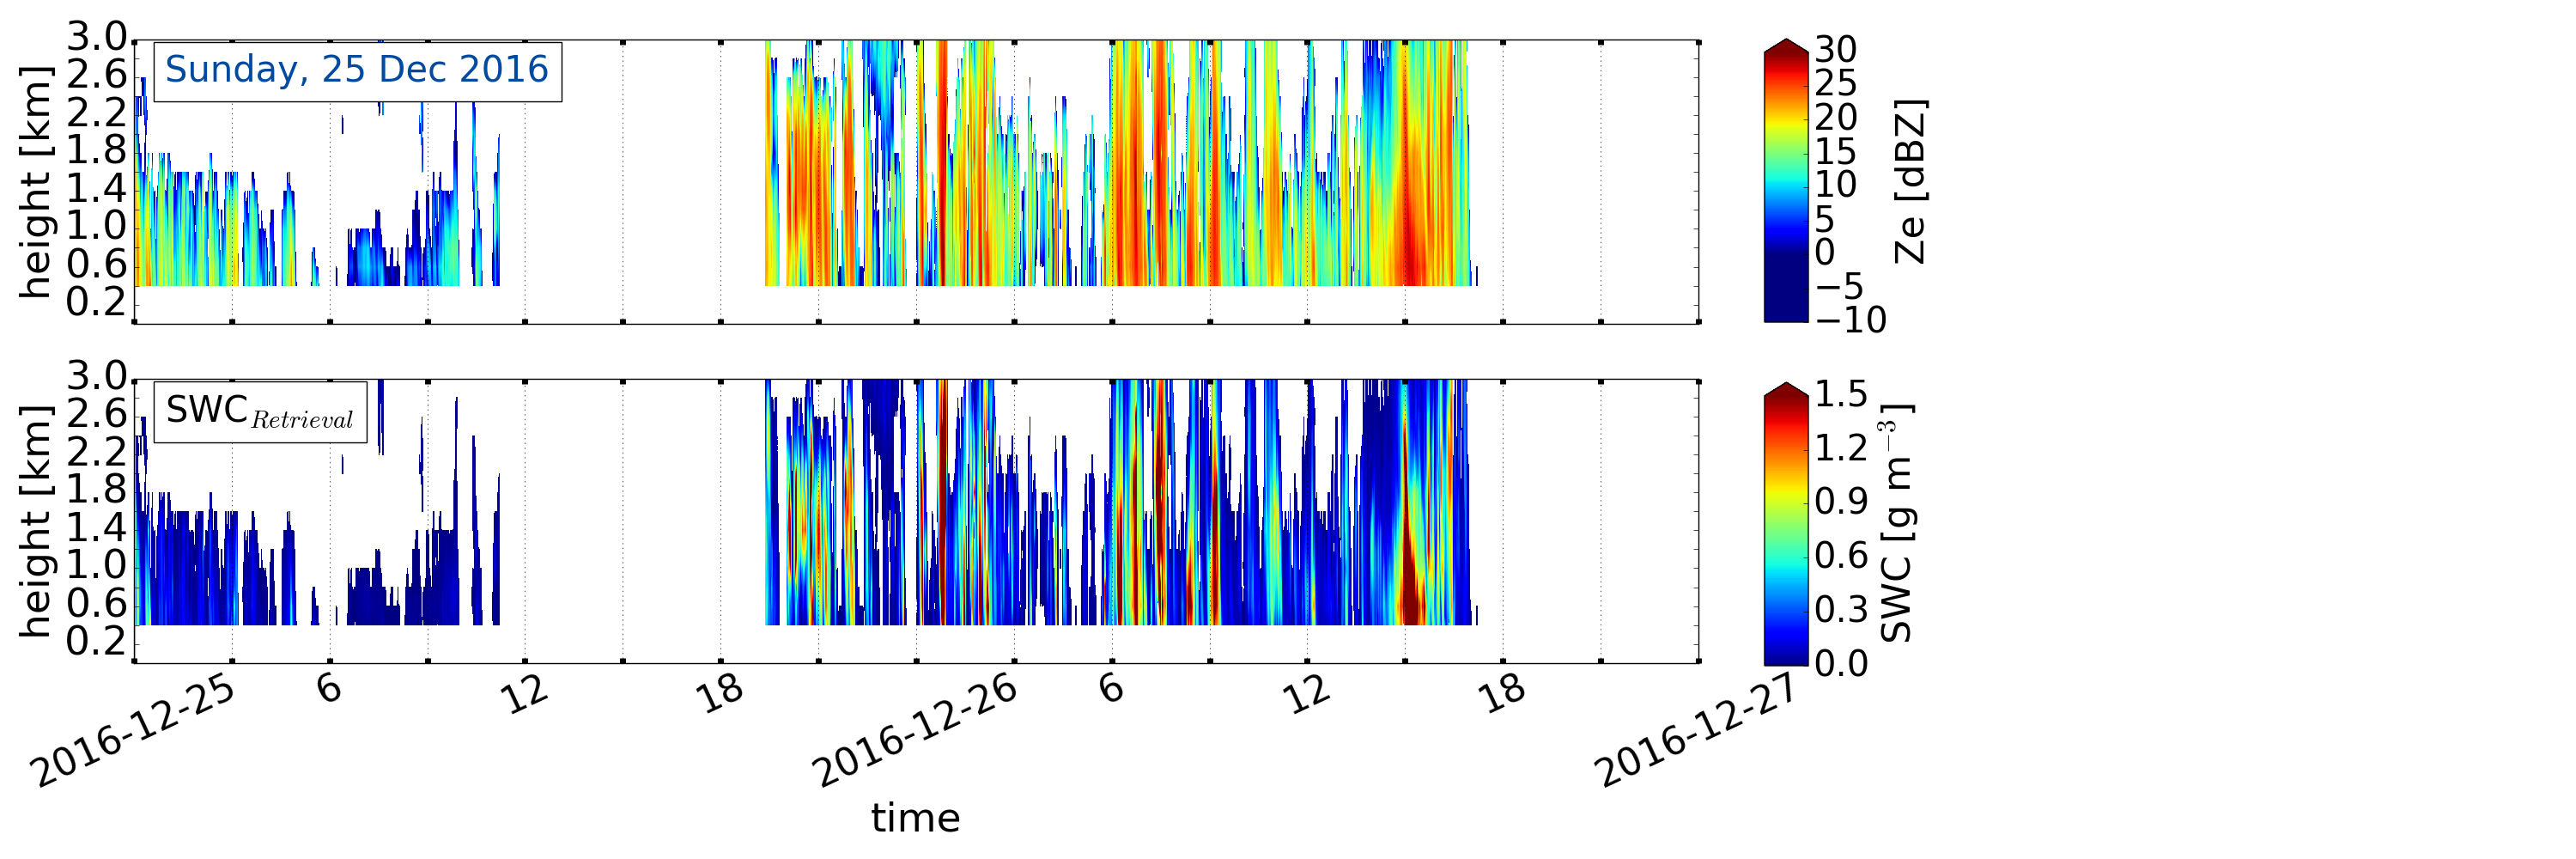
\includegraphics[trim={0.cm 2.2cm 19.cm 0.5cm},clip,width=0.9\textwidth]{./fig_obs_ret/20161225}
		\caption{}\label{fig:SWC:ret_25}
	\end{subfigure}
	% EM
	\begin{subfigure}[t]{\textwidth}
		\centering
		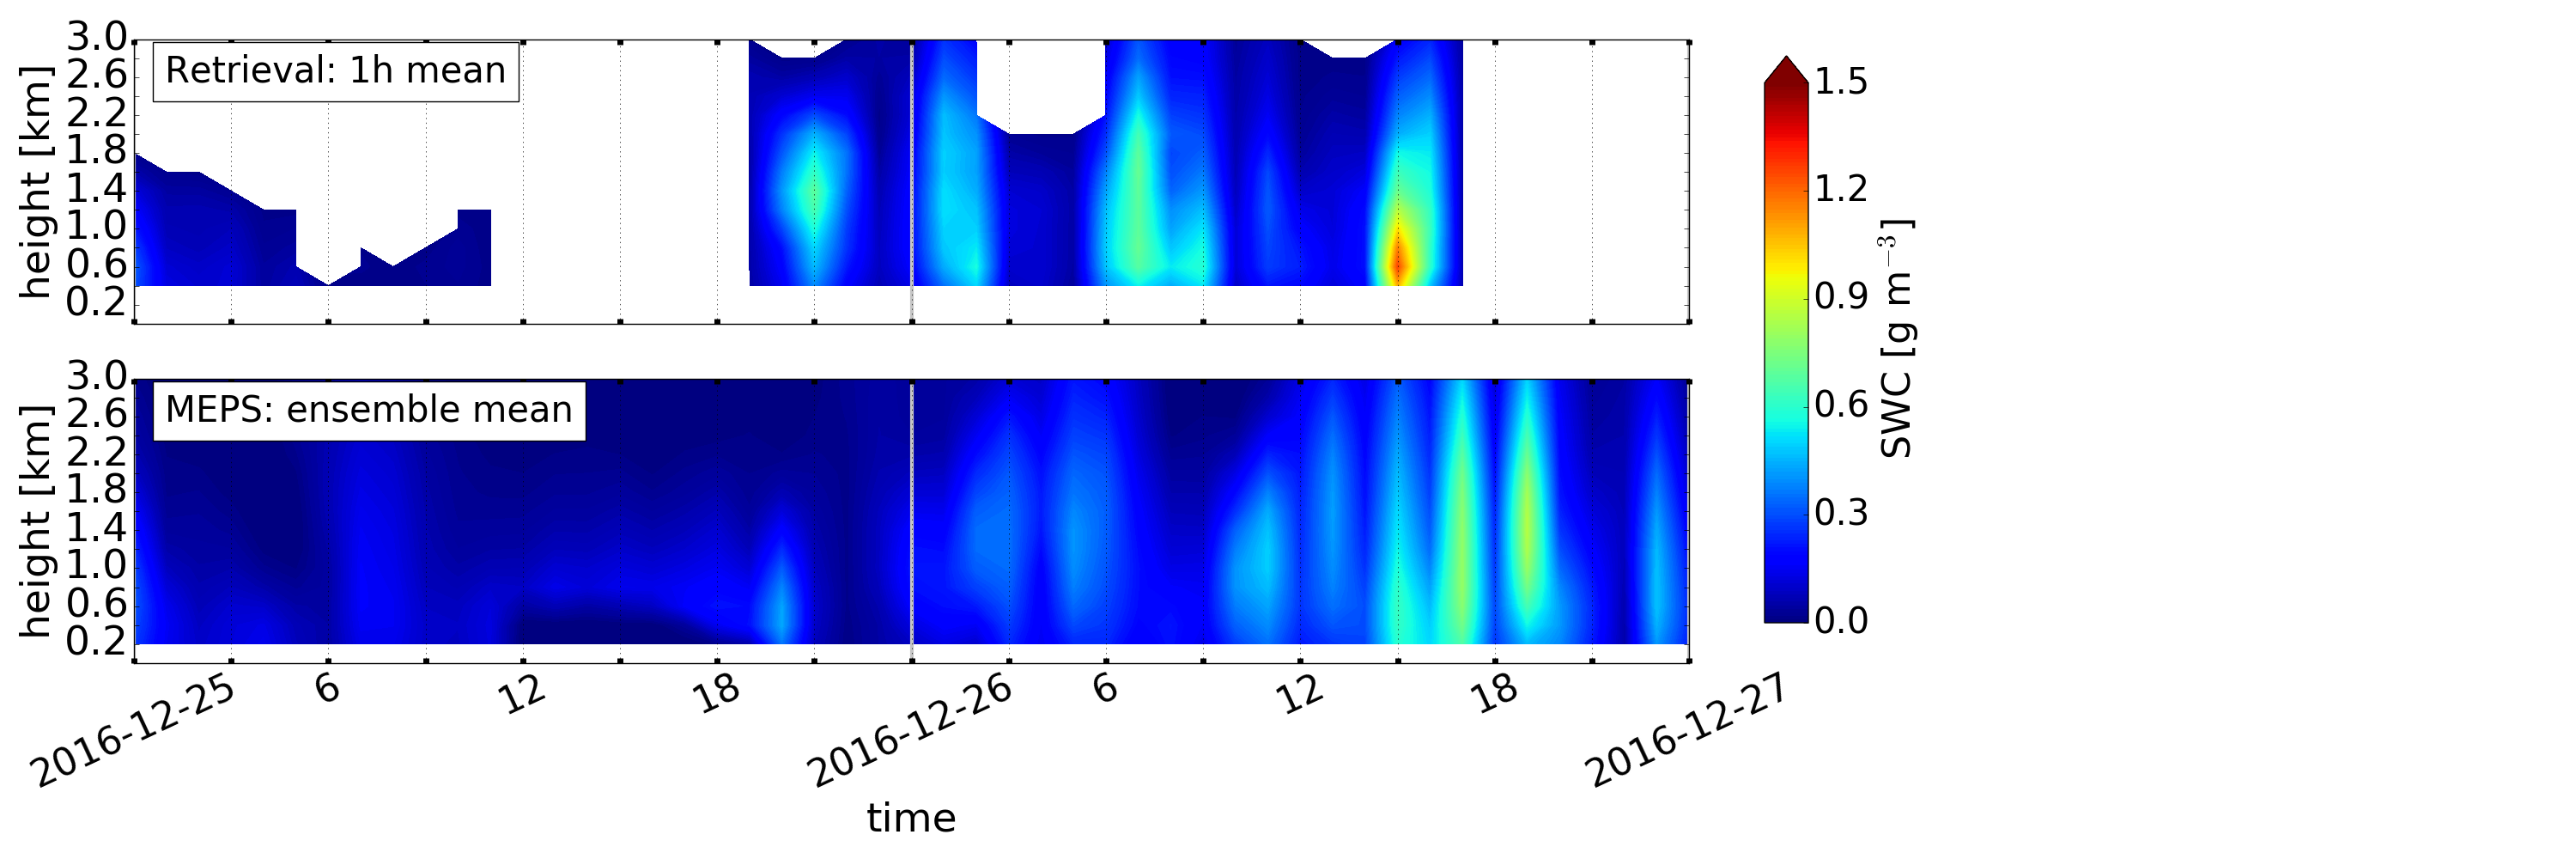
\includegraphics[trim={0.cm 2.2cm 19.cm 0.5cm},clip,width=0.9\textwidth]{./fig_vert_SWC_EM/20161225}
		\caption{}\label{fig:SWC_EM:25}
	\end{subfigure}
	% 3h
	\begin{subfigure}[t]{\textwidth}
		\centering
		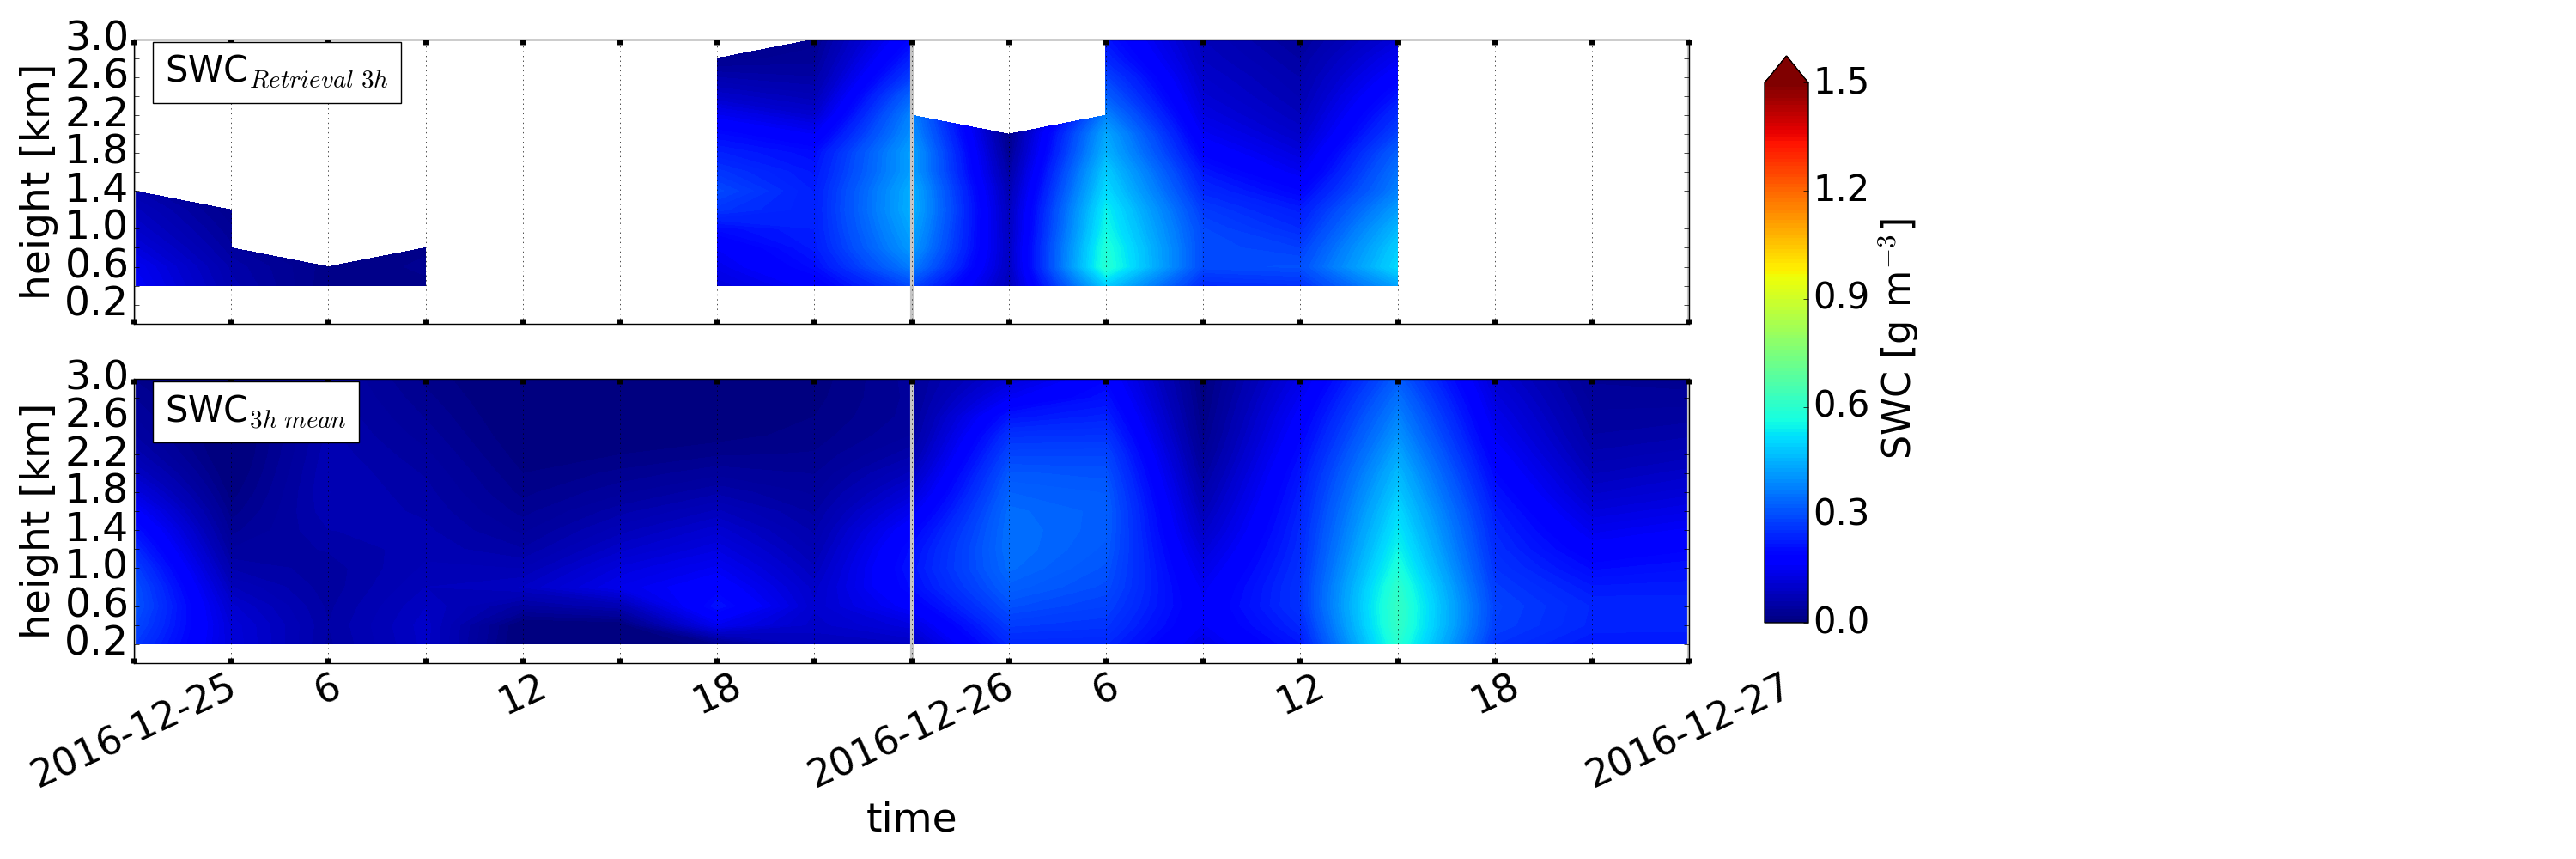
\includegraphics[trim={0.cm 0.8cm 19.cm 0.5cm},clip,width=0.9\textwidth]{./fig_vert_SWC_3h/20161225}
		\caption{}\label{fig:SWC3h:25}
	\end{subfigure}
	\caption{\textit{(Continued from previous page.)} Initialisation \SI{25}{\dec} at \SI{0}{\UTC}.}
\end{figure}
%%%%%%%%% image SWC retrieval MEPS 26 %%%%%%%%%%%%%%
\begin{figure}[H]\ContinuedFloat
	\centering
	% 25/12
	\begin{subfigure}[t]{\textwidth}
		\centering
		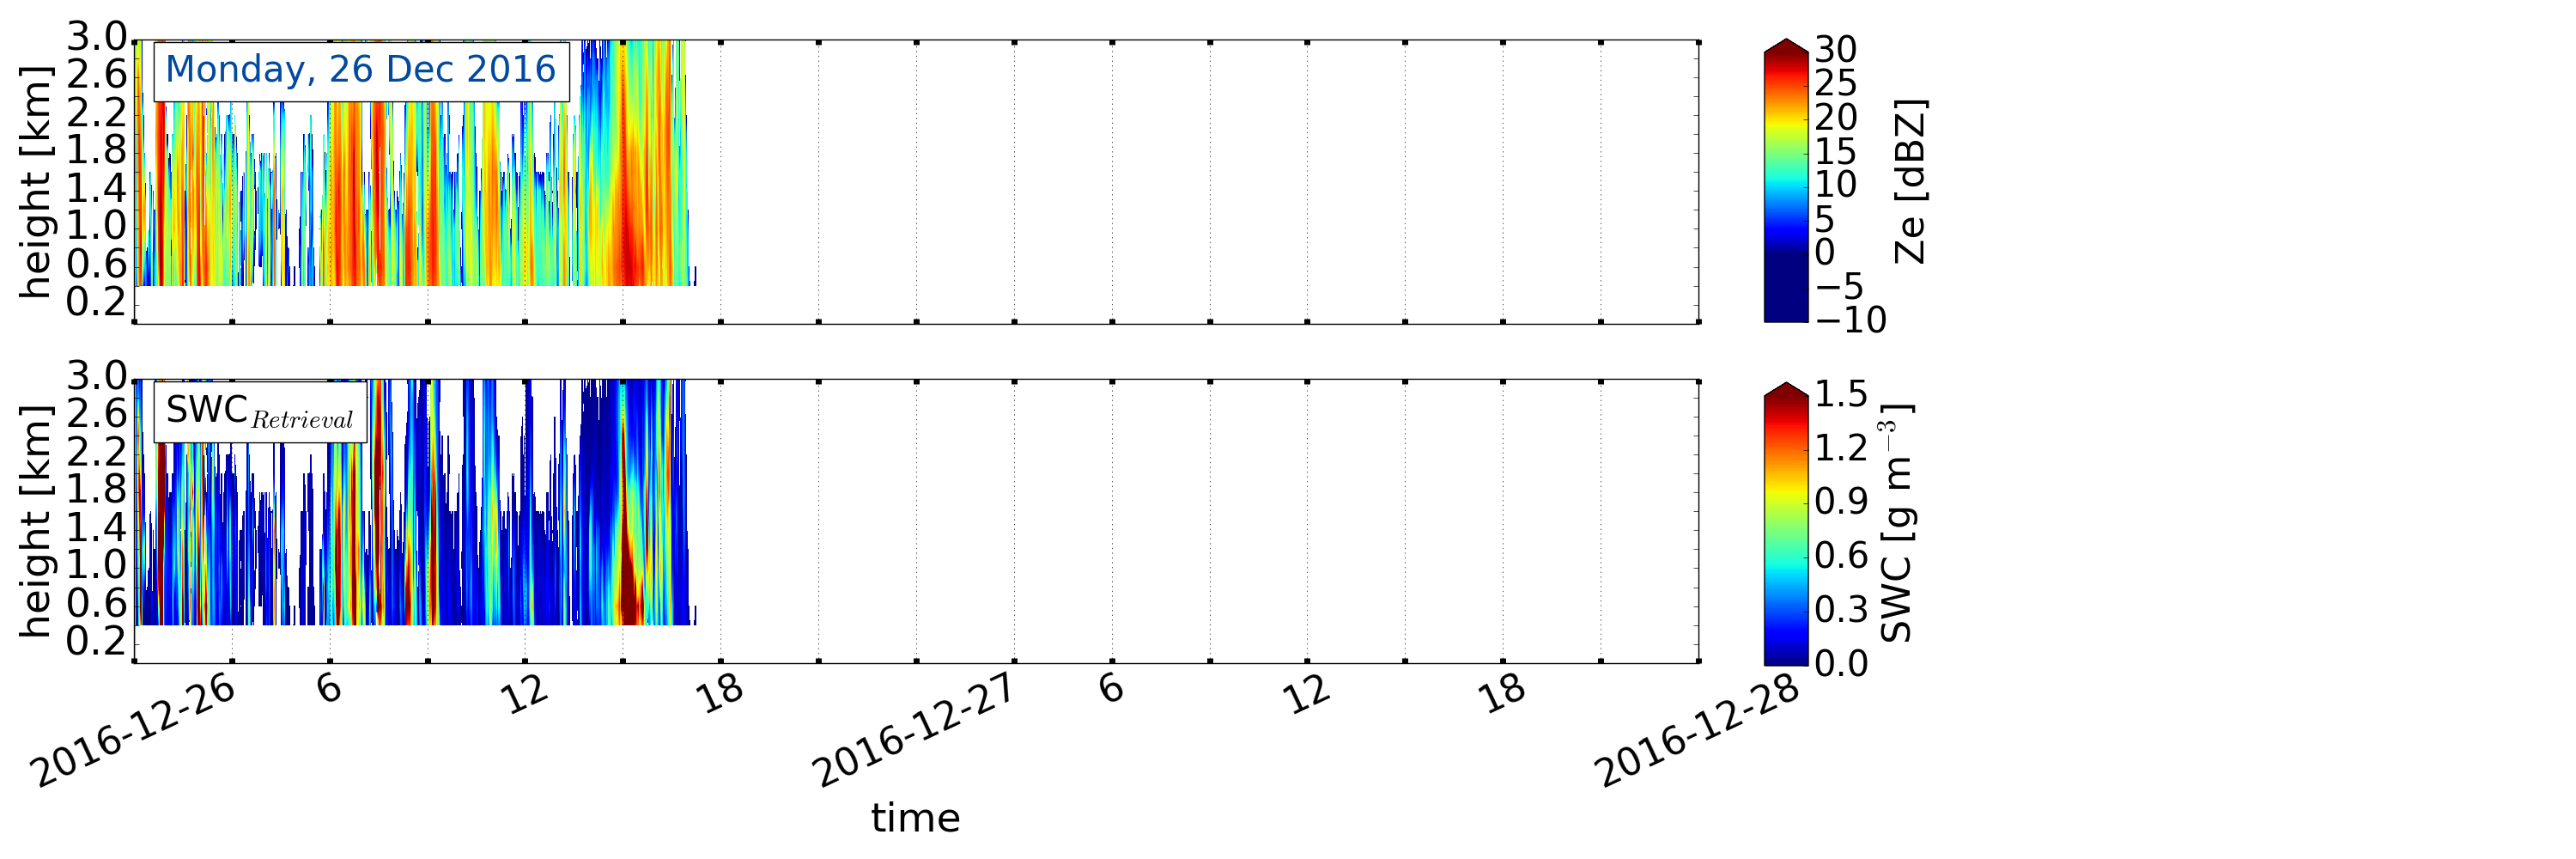
\includegraphics[trim={0.cm 2.2cm 19.cm 0.5cm},clip,width=0.9\textwidth]{./fig_obs_ret/20161226}
		\caption{}\label{fig:SWC:ret_26}
	\end{subfigure}
	% EM
	\begin{subfigure}[t]{\textwidth}
		\centering
		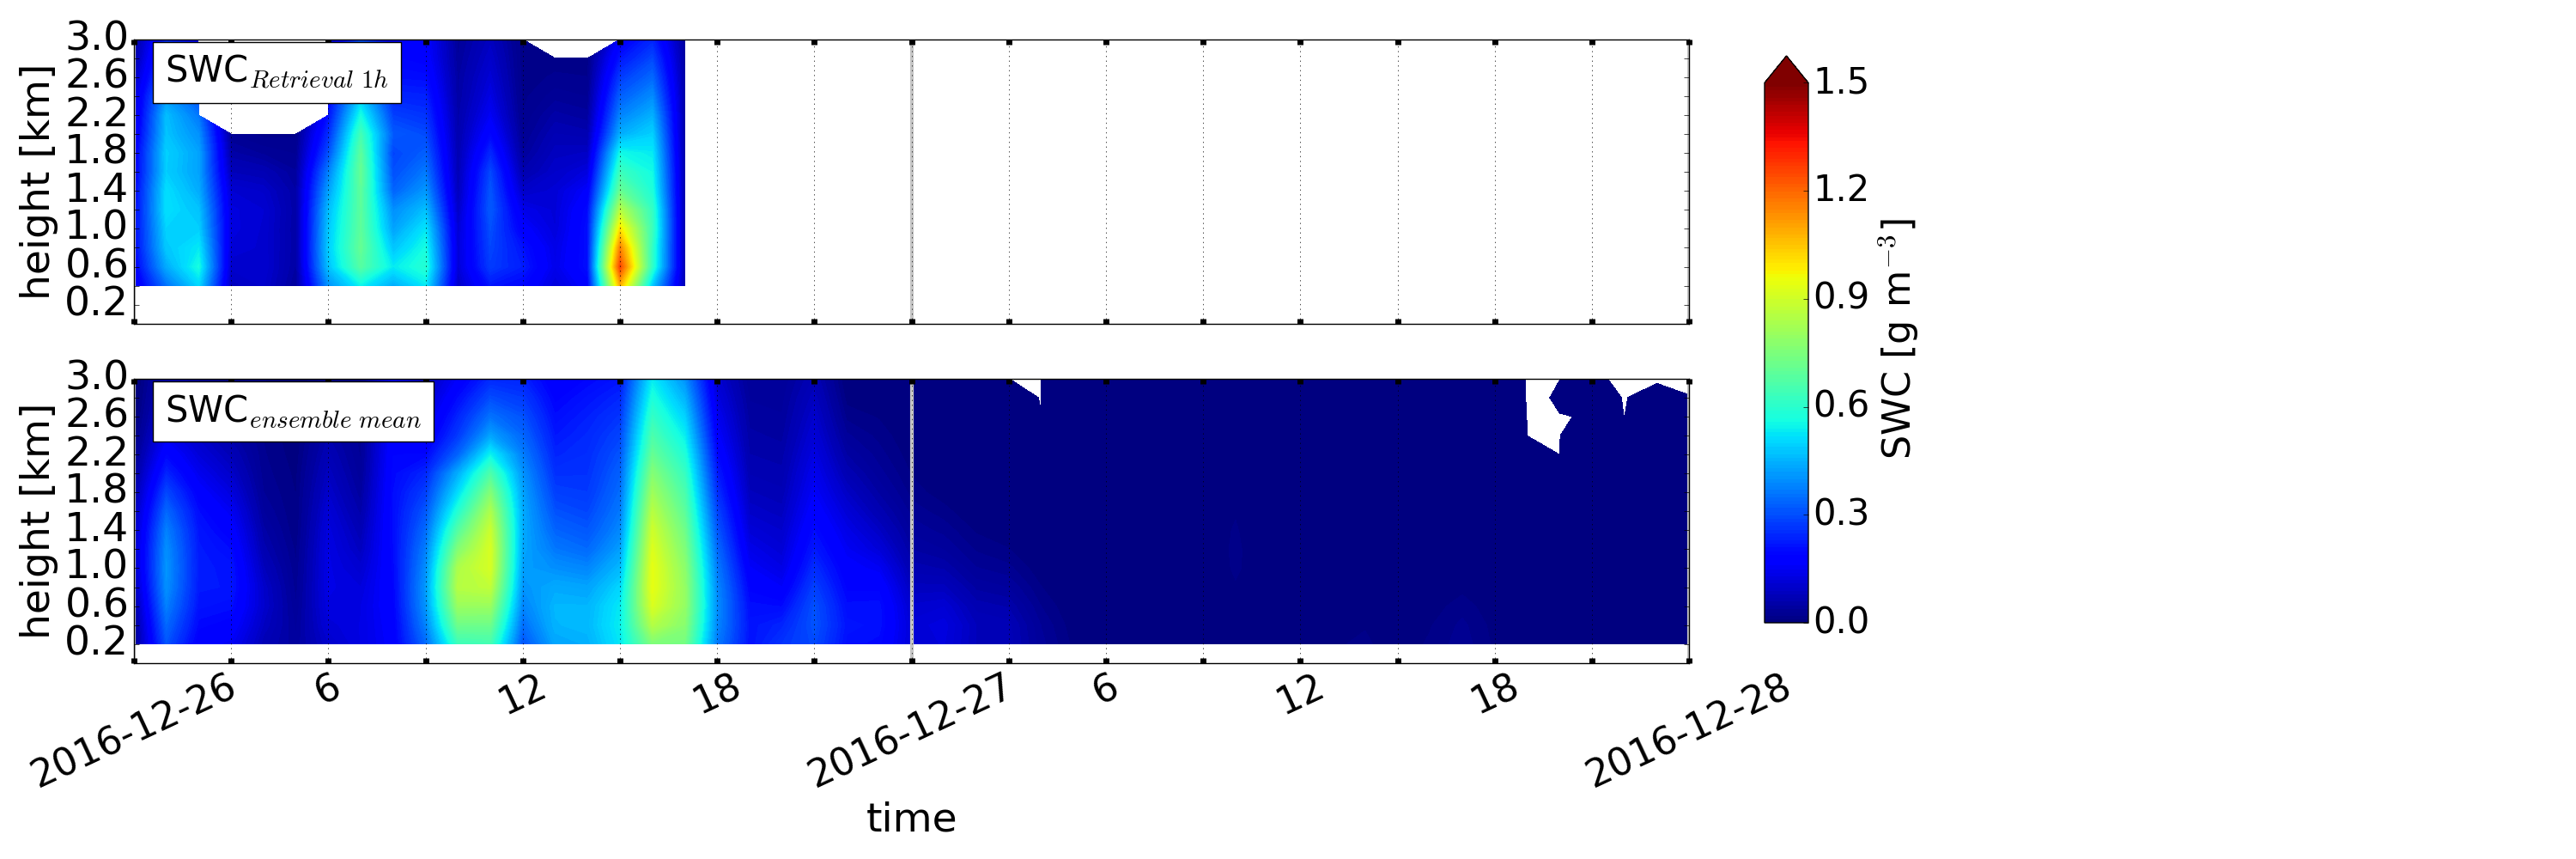
\includegraphics[trim={0.cm 2.2cm 19.cm 0.5cm},clip,width=0.9\textwidth]{./fig_vert_SWC_EM/20161226}
		\caption{}\label{fig:SWC_EM:26}
	\end{subfigure}
	% 3h
	\begin{subfigure}[t]{\textwidth}
		\centering
		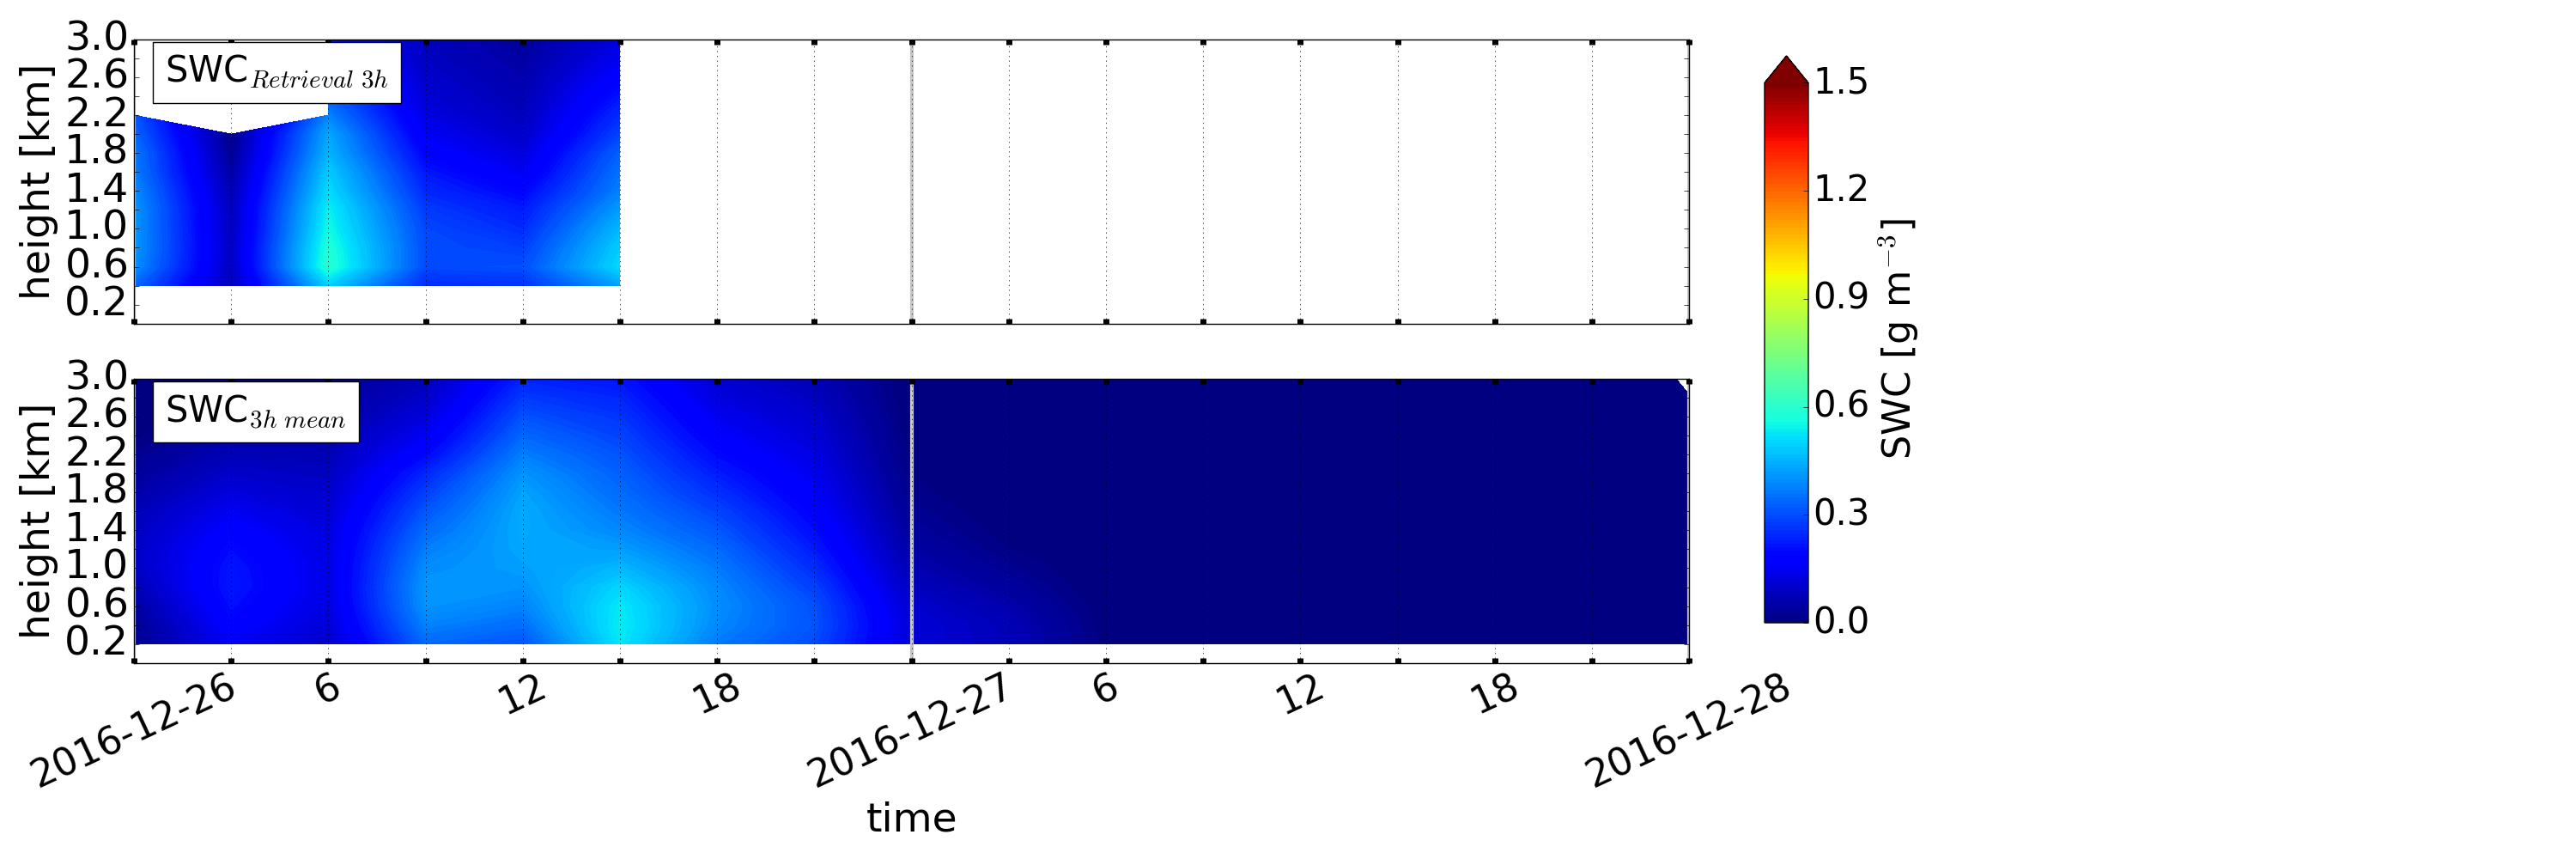
\includegraphics[trim={0.cm 0.8cm 19.cm 0.5cm},clip,width=0.9\textwidth]{./fig_vert_SWC_3h/20161226}
		\caption{}\label{fig:SWC3h:26}
	\end{subfigure}
	\caption{\textit{(Continued from previous page.)} Initialisation \SI{26}{\dec} at \SI{0}{\UTC}.}
\end{figure}
%%%%%%%%%%%%%%%%%%%%%%%%%%%%%%%%%%%%%%%%%%%%%%%%%%%%%%%%%%%%%%%%%%%%%%%%%
\noindent
In general, the forecasted instantaneous snow water content amount is weaker than the retrieved values for predictions on \SI{23}{\dec}. Hourly averages, only using the deterministic forecast and the first ensemble member show no occurrence of the occlusion passage on either day (\Cref{fig:SWC_1}). The variation of each initialisation ensemble member is given in \Cref{fig:EM09} for the respective day
%initialised on the respective day are given in \Cref{fig:EM09}. 
In \Cref{fig:EM09_22} the prediction for the occlusion passage is quite weak for all ensemble members 
\\
In the evening of \SI{23}{\dec}, the first perturbed ensemble member does not exist and hence little snow water content is predicted for the ensemble means especially for the hourly resolved mean \Cref{fig:SWC1h:22}). 
A comparison with \num{25} and \SI{26}{\dec} show the same result, when only the deterministic forecast and first perturbed member is used \Cref{fig:SWC1h:25} and \subref{fig:SWC1h:26}. 
\\ 
On \SI{26}{\dec}, only retrieves snow water content until the passage of the occlusion is observed (\Cref{fig:res:sfc_pres26,fig:res:sfc_temp26,fig:res:sfc_wd26,fig:res:sfc_ws26,fig:res:sfc_precip26}. The average of all ensemble members (\Cref{fig:SWC_EM:26}) as well as the three-hourly instantaneous SWC (\Cref{fig:SWC3h:26}) predict the frontal passage. 
Initialisations already \SI{39}{\hour} prior let assume that intense precipitation over a short time will occur (\Cref{fig:SWC_EM:25}, \subref{fig:SWC3h:25}). The variation of all members in \Cref{fig:EM09_25} and \subref{fig:EM09_26} indicate that almost all perturbed members would have predicted the precipitation around \SI{16}{\UTC}, but the ensemble mean weakens the result. 
On \num{25} and \SI{26}{\dec} high predicted SWC values are calculated for the deterministic forecast, than for any other ensemble member. 
This bias might have led to an overestimation at the surface on \SI{26}{\dec}, where the deterministic forecast indicates higher values than the perturbed members (\Cref{fig:sfc_acc26}). But in \Cref{fig:SWC1h:25} and \subref{fig:SWC1h:26} the amount of snow water content is very weak. 
Better estimations for predicted snowfall amount are displaye for the use of all ten ensemble member with either hourly or three hourly time resolution to creat the ensemble mean.
Still, the instantaneous average values of all ensemble members are much weaker than the retrieved SWC.
\\
%%%%%%% image liquid forecast 25 %%%%%%%%%%%%%%%%
\begin{figure}[t]
	\centering
	\begin{subfigure}[b]{\textwidth}
		\centering
		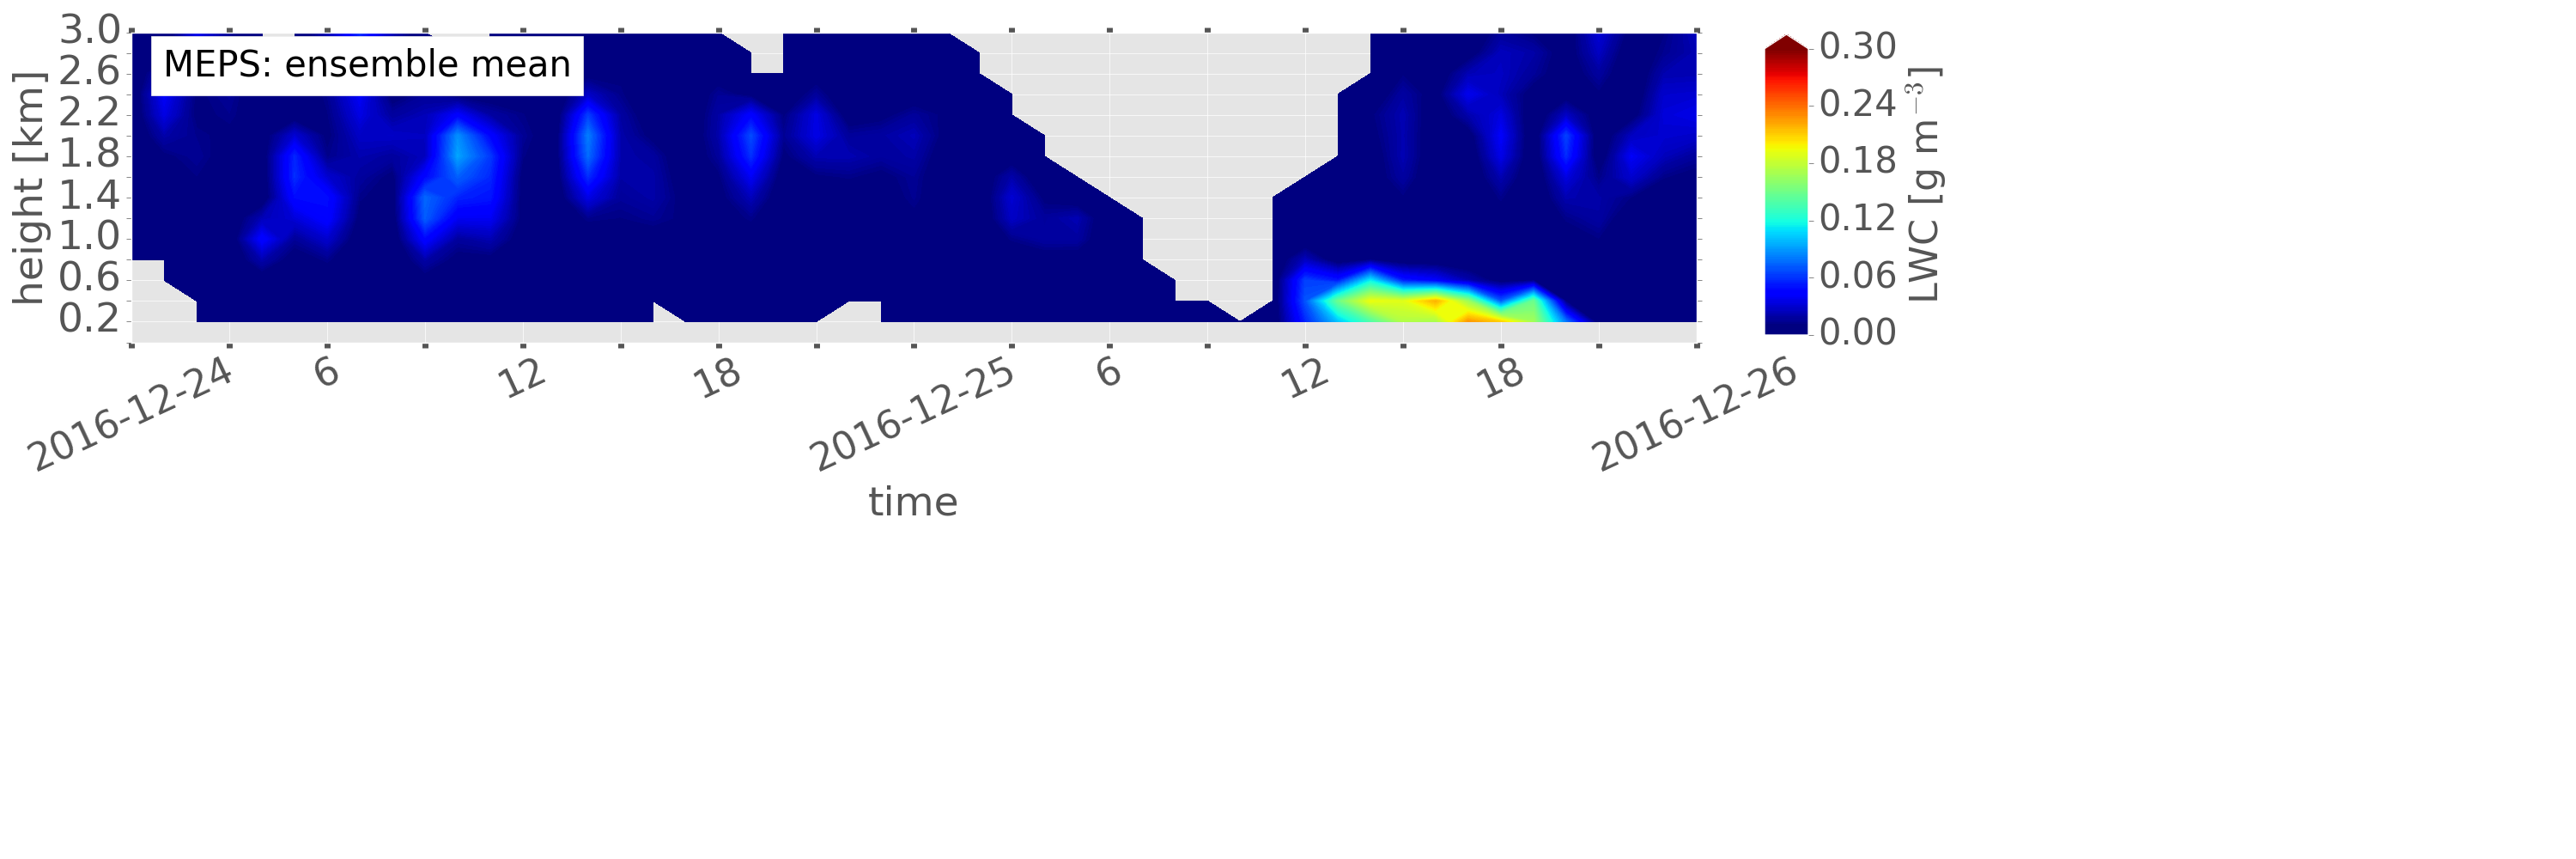
\includegraphics[trim={0.cm 11.5cm 18.5cm 0.4cm},clip,width=\textwidth]{./fig_vert_LWC_EM/20161224}
		\caption{}\label{fig:LWC:24}
	\end{subfigure}
	\begin{subfigure}[b]{\textwidth}
		\centering
		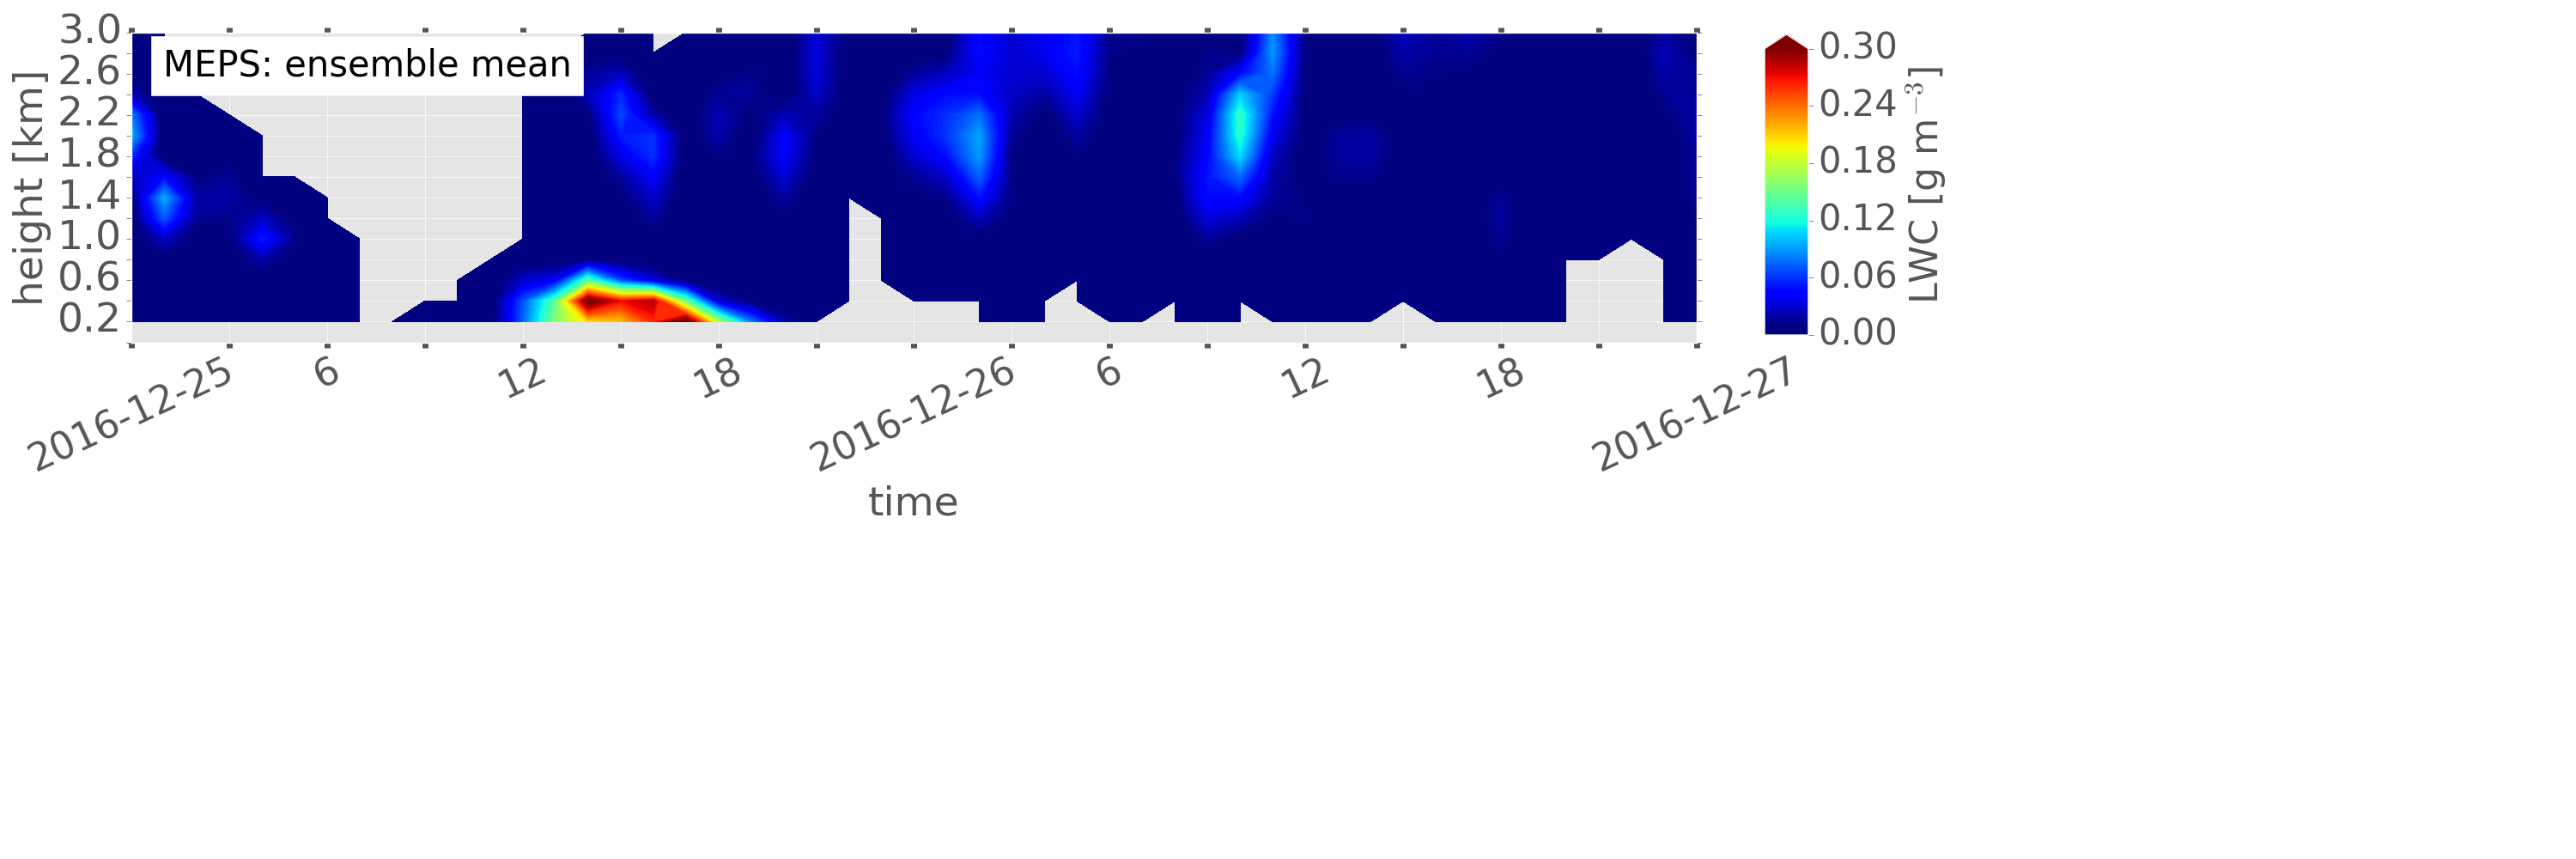
\includegraphics[trim={0.cm 10cm 18.5cm 0.4cm},clip,width=\textwidth]{./fig_vert_LWC_EM/20161225}
		\caption{}\label{fig:LWC:25}
	\end{subfigure}
	\caption{200m hourly averaged LWC forecast from MEPS with all ensemble members, neglecting missing values.
		Initialised on \SIlist{24;25}{\dec} at \SI{0}{\UTC}. Liquid water content according to the colorbar.}\label{fig:LWC:2425}
\end{figure}
%%%%%%%%%%%%%%%%%%%%%%%%%%%%%%%%%%%%%%%%%%%%%%
In the observations on \SI{25}{\dec}, patterns of possible liquid precipitation (\Cref{fig:res:obs_masc}) related to warm temperatures (\Cref{fig:res:sfc_temp25}) and high reflectivity (\Cref{fig:ret:refl25}) are shown, between \SIrange{12}{21}{\UTC}. High reflectivity values in \Cref{fig:ret:refl25} are present around \SI{18}{\UTC} with layer thickness up to \SI{1.2}{\km}. 
To see if liquid precipitation is predicted, the atmospheric cloud condensed water content and rainfall amount in model levels is summed (\Cref{fig:LWC:2425}). \Cref{fig:LWC:24} and \subref{fig:LWC:25} show liquid water content for initialisations on \SI{24}{\dec} or \SI{25}{\dec}, respectively. 
Positive surface temperatures were forecasted between \SIlist{12;21}{\UTC} (\Cref{fig:res:sfc_temp25}). Initialisations more than \SI{24}{\hour} prior show already the occurrence of the liquid layer (\Cref{fig:LWC:24}). \Cref{fig:LWC:24} or \subref{fig:LWC:25} show also a narrow liquid layer thickness up to \SI{800}{\metre}. 
\\
In Norwegian mountainous terrain this is an important forecast ability, since precipitation change can lead to a high risk for people. The avalanche danger increases with the precipitation change especially during high wind speeds \citep{hansen_warmer_2014}. Since MEPS forecasts the liquid layer correctly in thickness and duration it seems to be a good interaction between the surface model temperature and the temperature assimilation. 
This follows a high accuracy of MEPS and the positive impact of using a high resolution convective scheme model.
\\
%%% table verification %%%%%%%%%%%%%%%%%%%%%%%%%%%%%%%%%%%%%
\begin{table}[t!]
	\begin{center}
		\caption{Interpretation of the coefficient of variation for SWC.} \label{tab:verification}
		\begin{tabular}{lc|c}
			\hline\hline
			\multicolumn{2}{c|}{\textbf{Size of CV}} & {\textbf{Interpretation}} \\ 
			\multicolumn{2}{c|}{[\SI{}{\percent}]} & variability \\ \hline \hline 
			\multicolumn{2}{c|}{\numrange{0}{< 25}} & negligible  \\ \hline
			\multicolumn{2}{c|}{\numrange{25}{< 50}} & low \\ \hline
			\multicolumn{2}{c|}{\numrange{50}{< 75}} & moderate \\ \hline
			\multicolumn{2}{c|}{\numrange{75}{< 100}} & high \\ \hline
			\multicolumn{2}{c|}{\num{100} to $\infty$} & very high  \\ \hline \hline
		\end{tabular}
	\end{center}
\end{table}
%%%%%%%%%%%%%%%%%%%%%%%%%%%%%%%%%%%%%%%%%%%%%%%%%%%%%%%%%%%%%%%%%%%%%%%%%
\noindent
\\
%A validation of how well the forecast performed is difficult to do at this state, since the time resolution of MEPS is coarse compared to the observations. 
For the first glance operates MEPS well when compared to vertical observations, even though weaker ensemble mean estimates occur compared to the observations. One possibility to assess the variability of all ensemble member is with the use of the coefficient of variation (CV) described in \Cref{sec:ens_mean_spread}. 
\Cref{fig:vari:EM22,fig:vari:EM24,fig:vari:EM25,fig:vari:EM26} show the coefficient of variation for SWC. 
\\
The grey line in \Cref{fig:ens_vari} presents the ensemble mean of the hourly predicted SWC values. The darker the shading in \Cref{fig:ens_vari} the smaller the variation of the SWC relative to the mean. 
\\
MEPS data does not exist for all ten ensemble members on on \SI{23}{\dec}. No coefficient of variation is calculated for this day, since only six perturbed members were available. Therefore, the initialisation on \SI{22}{\dec} is used to validate the forecast. The interpretation of the coefficient of variation for SWC is presented in \Cref{tab:verification}.
%%%%%%% image variability %%%%%%%%%%%%%%%%
\begin{figure}[t!]
	\centering
	\begin{subfigure}[b]{\textwidth}
		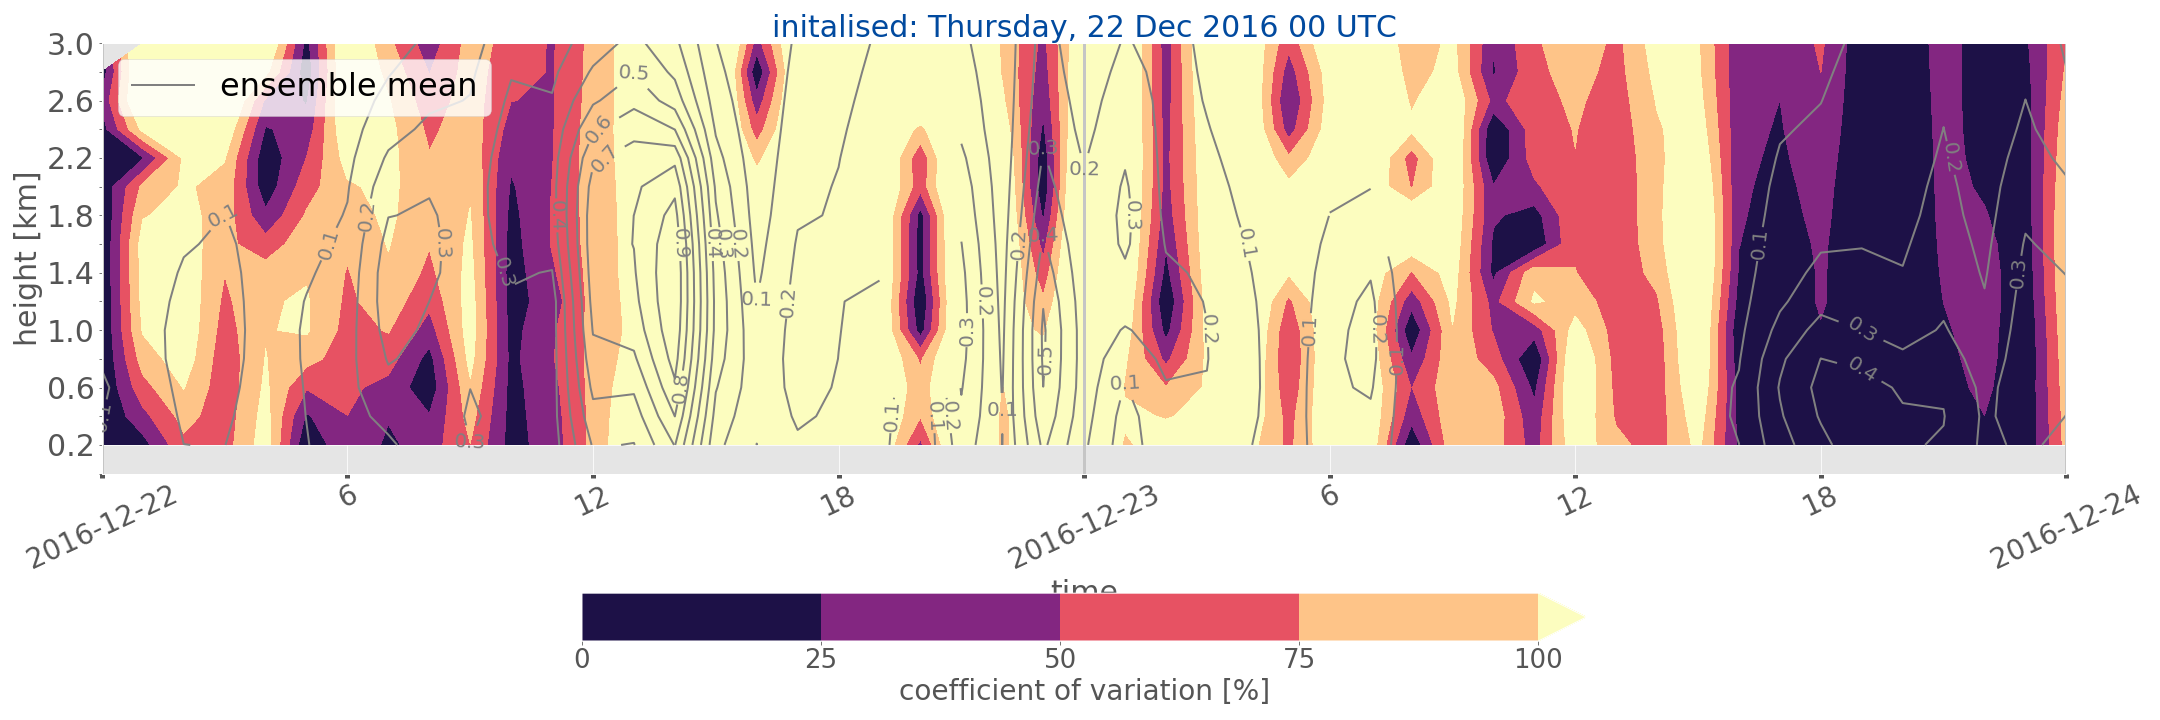
\includegraphics[trim={0cm 5cm 0cm 0cm},clip,width=\textwidth]{./fig_variation/20161222}
		\caption{}\label{fig:vari:EM22}
	\end{subfigure}
	\begin{subfigure}[b]{\textwidth}
		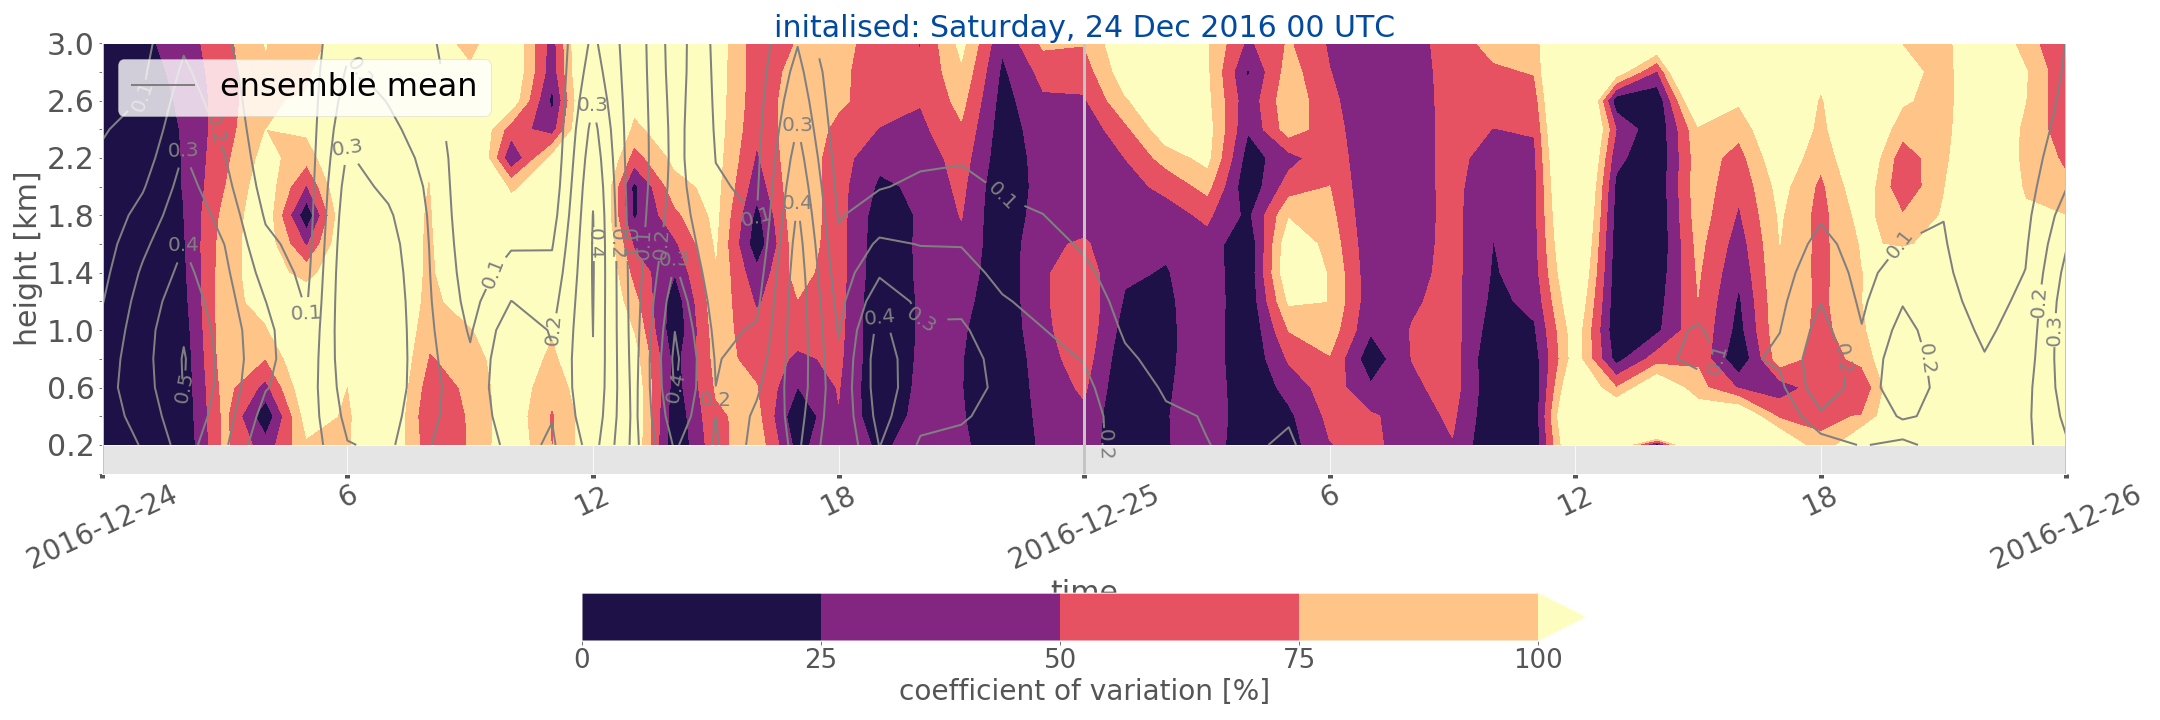
\includegraphics[trim={0cm 0cm 0cm 0cm},clip,width=\textwidth]{./fig_variation/20161224}
		\caption{}\label{fig:vari:EM24}
	\end{subfigure}
	\caption{SWC variation of the ten ensemble members of MEPS. The lighter the colour according to the colour bar the higher the variation between the perturbed ensemble members. In grey the ensemble mean of all ten members. For initialisations on \num{22} and \SI{24}{\dec}. \textit{Continued on next page.}}\label{fig:ens_vari}
\end{figure}
\begin{figure}[t!]\ContinuedFloat
	\begin{subfigure}[b]{\textwidth}
		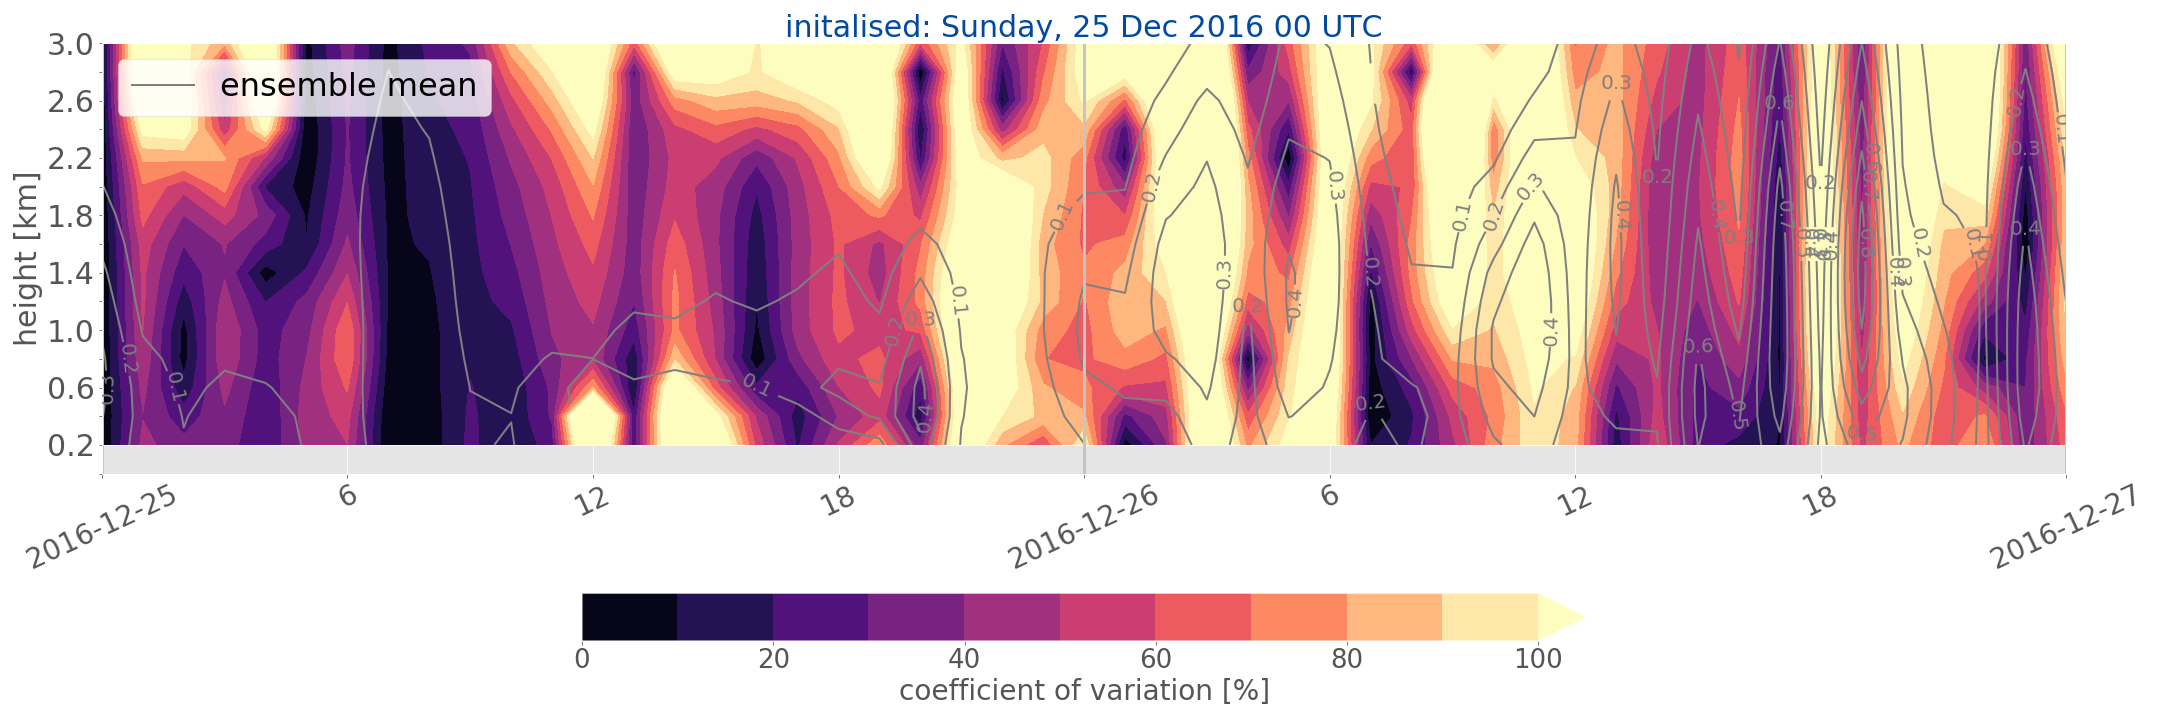
\includegraphics[trim={0cm 5cm 0cm 0cm},clip,width=\textwidth]{./fig_variation/20161225}
		\caption{}\label{fig:vari:EM25}
	\end{subfigure}
	\begin{subfigure}[b]{\textwidth}
		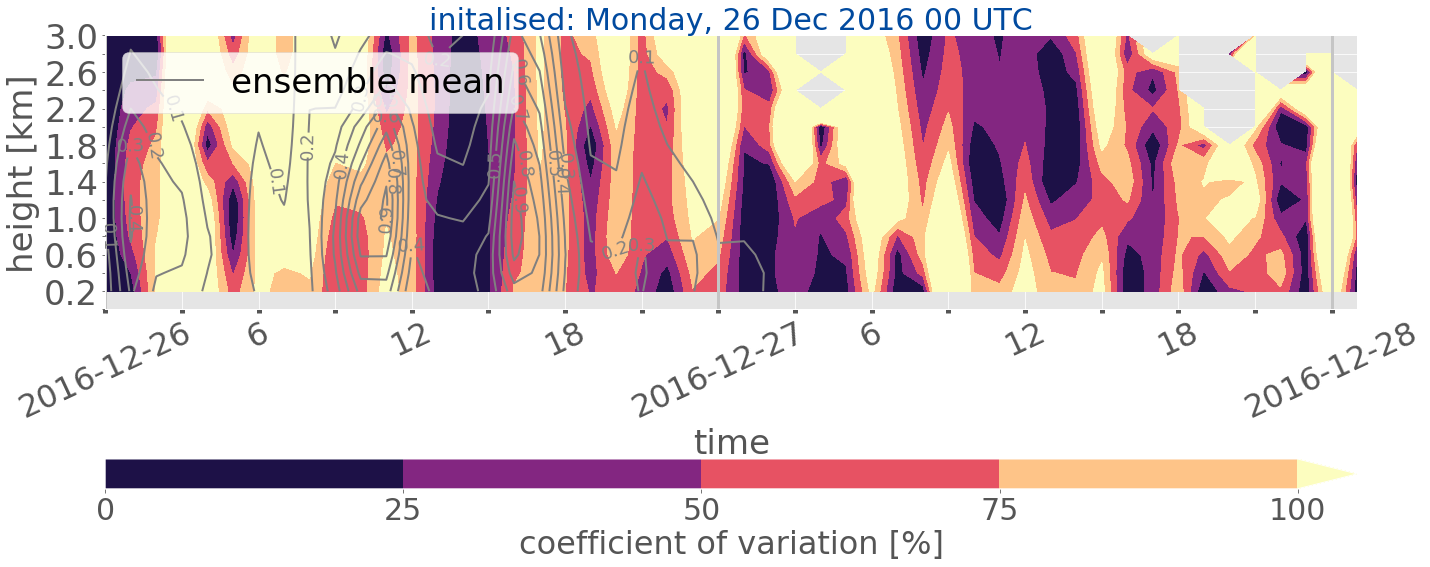
\includegraphics[trim={0cm 0cm 0cm 0cm},clip,width=\textwidth]{./fig_variation/20161226}
		\caption{}\label{fig:vari:EM26}
	\end{subfigure}
	\caption{\textit{(Continued from previous page.)} Initialisation \num{25} and \SI{26}{\dec}.}
\end{figure}
%%%%%%%%%%%%%%%%%%%%%%%%%%%%%%%%%%%%%%%%%%%%%
\noindent
\\
All ensemble members agree well with the occurrence of the up-slope storm on \SI{23}{\dec} after \SI{15}{\UTC} (\Cref{fig:EM09_22}). For prediction initialised on \SI{22}{\dec} the verification in \Cref{fig:vari:EM22} shows little variability below \SI{50}{\percent} and show a good agreement on the occurrence of snow precipitation. All ten ensemble members forecast the up-slope to occur after \SI{16}{\UTC}, compare \Cref{fig:EM09_22} and \subref{fig:EM09_23}. The comparison of only six ensemble members in \Cref{fig:EM09_23}, let assume that the variability between all ensemble members during the up-slope storm is low, but not as certain as for an initialisation on \SI{22}{\dec} at \SI{0}{\UTC}. 
The deterministic forecast (EM0) and ensemble member one in \Cref{fig:EM09_22} indicate peaks of high SWC before \SI{8}{\UTC}. The retrieved SWC on \SI{23}{\dec} had two peaks, one at around \SI{2}{\UTC} and another at \SI{4}{\UTC}. The deterministic forecast, initialised on \SI{22}{\dec} predicted a peak at \SIlist{2;6;8}{\UTC}, where the first perturbed ensemble member (EM1) has a strong SWC at \SI{7}{\UTC}. Overall seems a combination of the deterministic and first ensemble member of the  \SI{22}{\dec} initialisation to be a good forecast when comparing to the retrieved SWC in \Cref{fig:SWC:ret_22,fig:SWC_EM:22,fig:SWC3h:22,fig:SWC:ret_23,fig:SWC_EM:22,fig:SWC3h:22}.
\\
A larger variability between the ensemble members is shown for the evolution of the occlusion on \SI{26}{\dec} in \Cref{fig:vari:EM26}. In general, the \SI{25}{\dec} was a very weak snow storm with strong liquid precipitation observed between \SIlist{12;18}{\UTC}. Initialisations on \SI{25}{\dec} (\Cref{fig:vari:EM25}) present a lower variability for the transition after \SI{15}{\UTC} on \SI{26}{\dec} than initialisations less than \SI{24}{\hour} prior. Therefore, an increase of variability after shorter time is given rather than long lead time (\SI{48}{\hour}). \Cref{fig:SWC:ret_24,fig:SWC_EM:24,fig:SWC3h:24} and \Cref{fig:SWC:ret_25,fig:SWC_EM:25,fig:SWC3h:25} give a low value of predicted SWC in the course of a day. As \Cref{fig:vari:EM24} indicates is the forecast accuracy very high up to \SI{1.8}{\km} until noon, this is when liquid precipitation was measured. The depth of the liquid layer was up to \SI{0.8}{\km} in \Cref{fig:LWC:24} and \ref{fig:LWC:25}. The variation coefficient (\Cref{fig:vari:EM24} and \ref{fig:vari:EM25}) has a large disagreement below \SI{0.8}{\km}, but above the variability is between the members not existing or low. Initialisation on \SI{24}{\dec} show weak snow water content peak in \Cref{fig:SWC_EM:24} and \subref{fig:SWC3h:24} at \SI{18}{\UTC}, which had a moderate variability (\Cref{tab:verification}, \Cref{fig:vari:EM24}). Afterwards it is very high. Initialisation on \SI{25}{\dec} the forecast variability is low until noon (\Cref{fig:vari:EM25}). While liquid precipitation was monitored the variability in the lower layer is first very high and shortly before \SI{18}{\UTC} not existing. A high agreement for the SWC peak at \SI{20}{\UTC} up to \SI{0.8}{\km} exists in \Cref{fig:vari:EM25} and decreases to be moderate above. 
\\
\Cref{fig:SWC_EM:25} and \subref{fig:SWC3h:25} would suggest a continues pulsing of the storm. The two peaks around \SI{18}{\UTC} (\Cref{fig:SWC_EM:25}) are predicted with a negligible and moderate variability in \Cref{fig:ens_vari25}. The SWC peaks at around \SIlist{3;5}{\UTC} show a very high variability. \Cref{fig:EM09_25} displays that four out of ten ensemble members would agree with the peaked event around \SI{5}{\UTC}. Whereas the peak at \SI{3}{\UTC} is dominated by the strong predicted SWC of the deterministic forecast, which follows the high variation in \Cref{fig:vari:EM25}. 
Initialisation on \SI{26}{\dec} follow that the SWC peak at \SI{1}{\UTC} is related to a moderate variability of the ensemble members. Low forecast accuracy is shown for the SWC between \SIrange{9}{12}{\UTC} and the one between \SIrange{15}{18}{\UTC} has a low to moderate variability between the members.  When looking at \Cref{fig:EM09_26} might this disagreement be related to the colourful variation of the vertical predicted SWC. There seems to be no agreement between the different members about the incidence of the SWC peaks. The high conflict for the CV before noon is most likely related to the high SWC of the deterministic SWC.
\\
Again, this is not a fair comparison since hourly instantaneous values are used and there might be a time delay of half an hour about the development of boundaries which would follow it is not seen in the model forecast. 
\\
\\
One question to answer in this work is if the operational model MEPS estimates large scale features correctly. As discussed here and in \Cref{sec:res:large_scale_sfc} it seems that the model is able to cover the development of large scale features and its associated precipitation. Even with the intensification of the storm MEPS seem to be able to predict extreme events for vertical snowfall such as the 2016 Christmas extreme event, but might have some issues predicting transitions of frontal boundaries as well as associated precipitation at the surface. 
\\
MEPS is also able to distinguish between liquid and solid precipitation in layer thickness and duration for time resolution of one hour. This can be a major advantage since a change in temperature and associated precipitation transformation can lead to high safety issues in the Norwegian mountains, especially during winter. With the knowledge more than \SI{24}{\hour} prior can risk notice be send out to the population and rescue teams can prepare in advance. Furthermore, roads and train tracks can be closed to increase the safety. 
\\
The here presented results are a first look, trying to compare a mesoscale ensemble member forecast system (MEPS) with vertical in-situ measurement for snowfall.
\\
The next section will go into detail, how the local orography at Haukeliseter may influence frozen precipitation, and how MEPS's representation of the topography may affect it. 
%%%%%%%%%%%%%%%%%%%%%%%%%%%%%%%%%%%%%%%%%%%%%%%%%%%%%


%%%%%%%%% Local affects %%%%%%%%%%%%%%
\subsection{Orographic influence on precipitation}\label{sec:res:oro_infl}
The Haukeliseter site is suspended to high wind speeds during the winter. The previous results in \Cref{sec:res:large_scale_sfc}, \ref{sec:sfc_acc}, \ref{sec:res:large_scale_vert} have shown, that wind plays an important role for the precipitation at Haukeliseter. The mountain plateau is surrounded by higher mountains to the west and more open to the south east (\Cref{fig:res:Haukeli}), this orography seems to influence the vertical precipitation pattern. The correlation between wind speed observations and forecast show an overestimation of predicted wind speed throughout the event (\Cref{fig:res:sfc_ws21}, \subref{fig:res:sfc_ws23}, \subref{fig:res:sfc_ws25} and \subref{fig:res:sfc_ws26}). \citet{muller_arome-metcoop:_2017} already mentioned the weakness of too strong wind prediction in AROME-MetCoOp, the previous operational deterministic version of MEPS.
\\
\Cref{fig:res:MEPS_Haukeli} shows the MEPS resolution and its \SI{2.5}{\km} grid cells around the Haukeliseter site. 
%The complex terrain represented in the model could have followed a local misplacement of a precipitation cell by a few kilometres and followed an estimation of more accumulation at the site after noon.
The complex terrain and its representation in MEPS might have followed the overestimation of accumulation. In this thesis the closest grid point to the Haukeliseter measurement site is used. Alternatively, the use of an average of the grid points surrounding the Haukeliseter site could lead to a solution that is closer to the truth and must be evaluated further.
\\
On \num{21} and \SI{23}{\dec} wind directions from the south-east and south were observed, respectively. As earlier discussed in\Cref{sec:res:large_scale_sfc} and \ref{sec:res:large_scale_vert} the wind change is associated with the occlusion passage on \SI{23}{\dec} (\Cref{fig:DT23} and \ref{fig:GP23}). 
The wind direction on \SI{21}{\dec} in \Cref{fig:res:sfc_wd21} change was also related to the large scale synoptic flow but is not associated to a frontal boundary. A comparison with the large scale weather analysis from ECMWF shows, that the large scale surface wind is from the south-west at \SI{6}{\UTC} on \SI{21}{\dec} (not shown) and has changed to west at \SI{12}{\UTC} (\Cref{fig:GP21}). The observations at the Haukeliseter site show between \SIlist{6;12}{\UTC} wind from south-east, while the predicted wind direction is from south in \Cref{fig:res:sfc_wd21}. The local wind direction influenced the precipitation pattern in the vertical on \num{21} and \SI{23}{\dec}, in the matter that a more consistent storm structure was observed and predicted between \SIrange{9}{12} {\UTC} (\Cref{fig:SWC:ret_21,fig:SWC_EM:21,fig:SWC3h:21}). 
% %%%%%%% image location %%%%%%%%%%%%%%%%
\begin{figure}[H]
	\begin{tabular}[t]{cc}
		\begin{tabular}[t]{c}
			\begin{subfigure}[b]{0.8\columnwidth}
				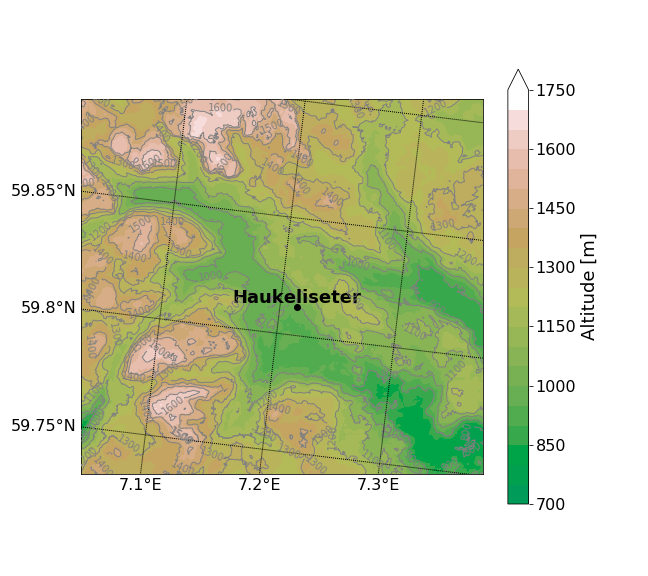
\includegraphics[trim={.3cm 2.2cm 5.5cm 2.4cm},clip,width=0.88\textwidth]{./fig_Norway/elevation_Haukeli}
				\caption{}\label{fig:res:Haukeli}
			\end{subfigure}\\
			\begin{subfigure}[b]{0.8\columnwidth}
				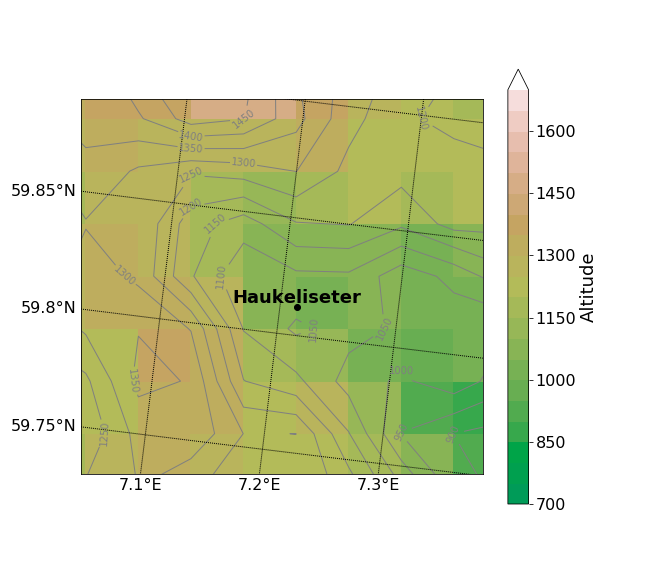
\includegraphics[trim={.3cm 2.2cm 5.5cm 2.4cm},clip,width=0.88\textwidth]{./fig_Norway/MEPS_elevation_Haukeli}
				\caption{}\label{fig:res:MEPS_Haukeli}
			\end{subfigure}
		\end{tabular}
		&
		\begin{subfigure}[t]{0.18\columnwidth}
			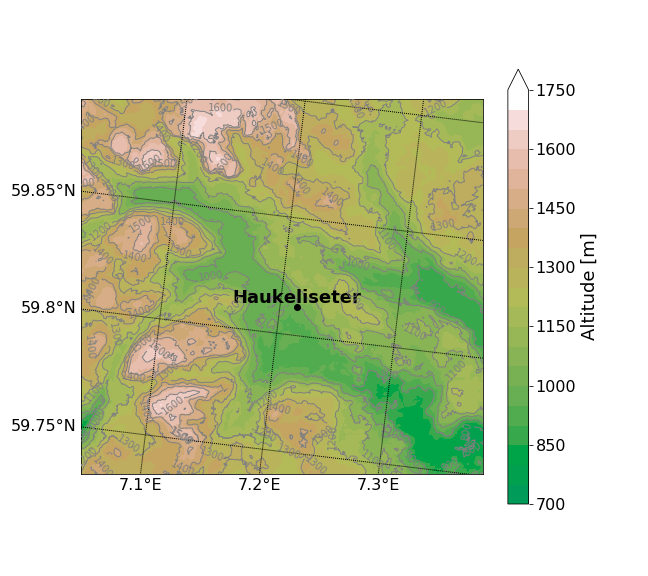
\includegraphics[trim={17.5cm 2.2cm 1.8cm 2.4cm},clip,width=0.9\textwidth]{./fig_Norway/elevation_Haukeli}
		\end{subfigure}
	\end{tabular}
	\caption{Topography around Haukeliseter. In \protect\subref{fig:res:Haukeli} the DTM 10 Terrain Model (UTM33) from \cite{geonorge_dtm_2018}. Contours and shading according to the colorbar. \protect\subref{fig:res:MEPS_Haukeli}: Representation of the topography around the measurement site Haukeliseter in MEPS. Contours and shading present the elevation of the grid cells.}\label{fig:res:topo}
\end{figure}
%%%%%%%%%%%%%%%%%%%%%%%%%%%%%%%%%%%%%%%%%%%%%%
\noindent
\\
Both days show a more consistent storm structure with not as intense snow water content than for storm patterns from the west such as on \SI{24}{\dec} (\Cref{fig:SWC:ret_24,fig:SWC_EM:24,fig:SWC3h:24}). 
\Cref{fig:res:Haukeli} presents the local topography around Haukeliseter and \Cref{fig:res:MEPS_Haukeli} shows the topography resolved by MEPS. 
MEPS is able to cover some of the complex structure around the site (\Cref{fig:res:MEPS_Haukeli}), with the higher mountain to the west and the valley to the south-east (\Cref{fig:res:Haukeli}). 
The forecast model seems to forecast the wind direction overall well, only on \SI{21}{\dec} before \SI{10}{\UTC} is a south-west instead of a south-east wind predicted. It displays that even if the large scale wind is from the south-west the local wind is rather from the south or south-east (\Cref{fig:GP21}).
\\
\Cref{fig:scat:wd2426} shows a good correlation for west winds, but on the other side, southerly winds seem to be troublesome to predict for MEPS. \Cref{fig:scat:wd2123} indicates an unbalance for south-westerly winds. While south-easterly winds (along the valley) are observed at Haukeliseter predicts MEPS the \SI{10}{\metre} wind to be south-westerly. 
\\
\Cref{fig:res:topo} shows the comparison between the orography and the resolved topography by MEPS. Observed south-easterly winds are forced along the valley, directed in south-east. MEPS resolves it in the way, that the wind is south-westerly. \Cref{fig:res:MEPS_Haukeli} displays a high mountain to the west of the station and a small one to the south. \SI{10}{\metre} wind predicted by MEPS is predicted to blow between these two elevations.
%%%%%%%%% image SWC retrieval MEPS 21 %%%%%%%%%%%%%%
\begin{figure}[H]
	\centering
	% 21/12
	\begin{subfigure}[t]{\textwidth}
		\centering
		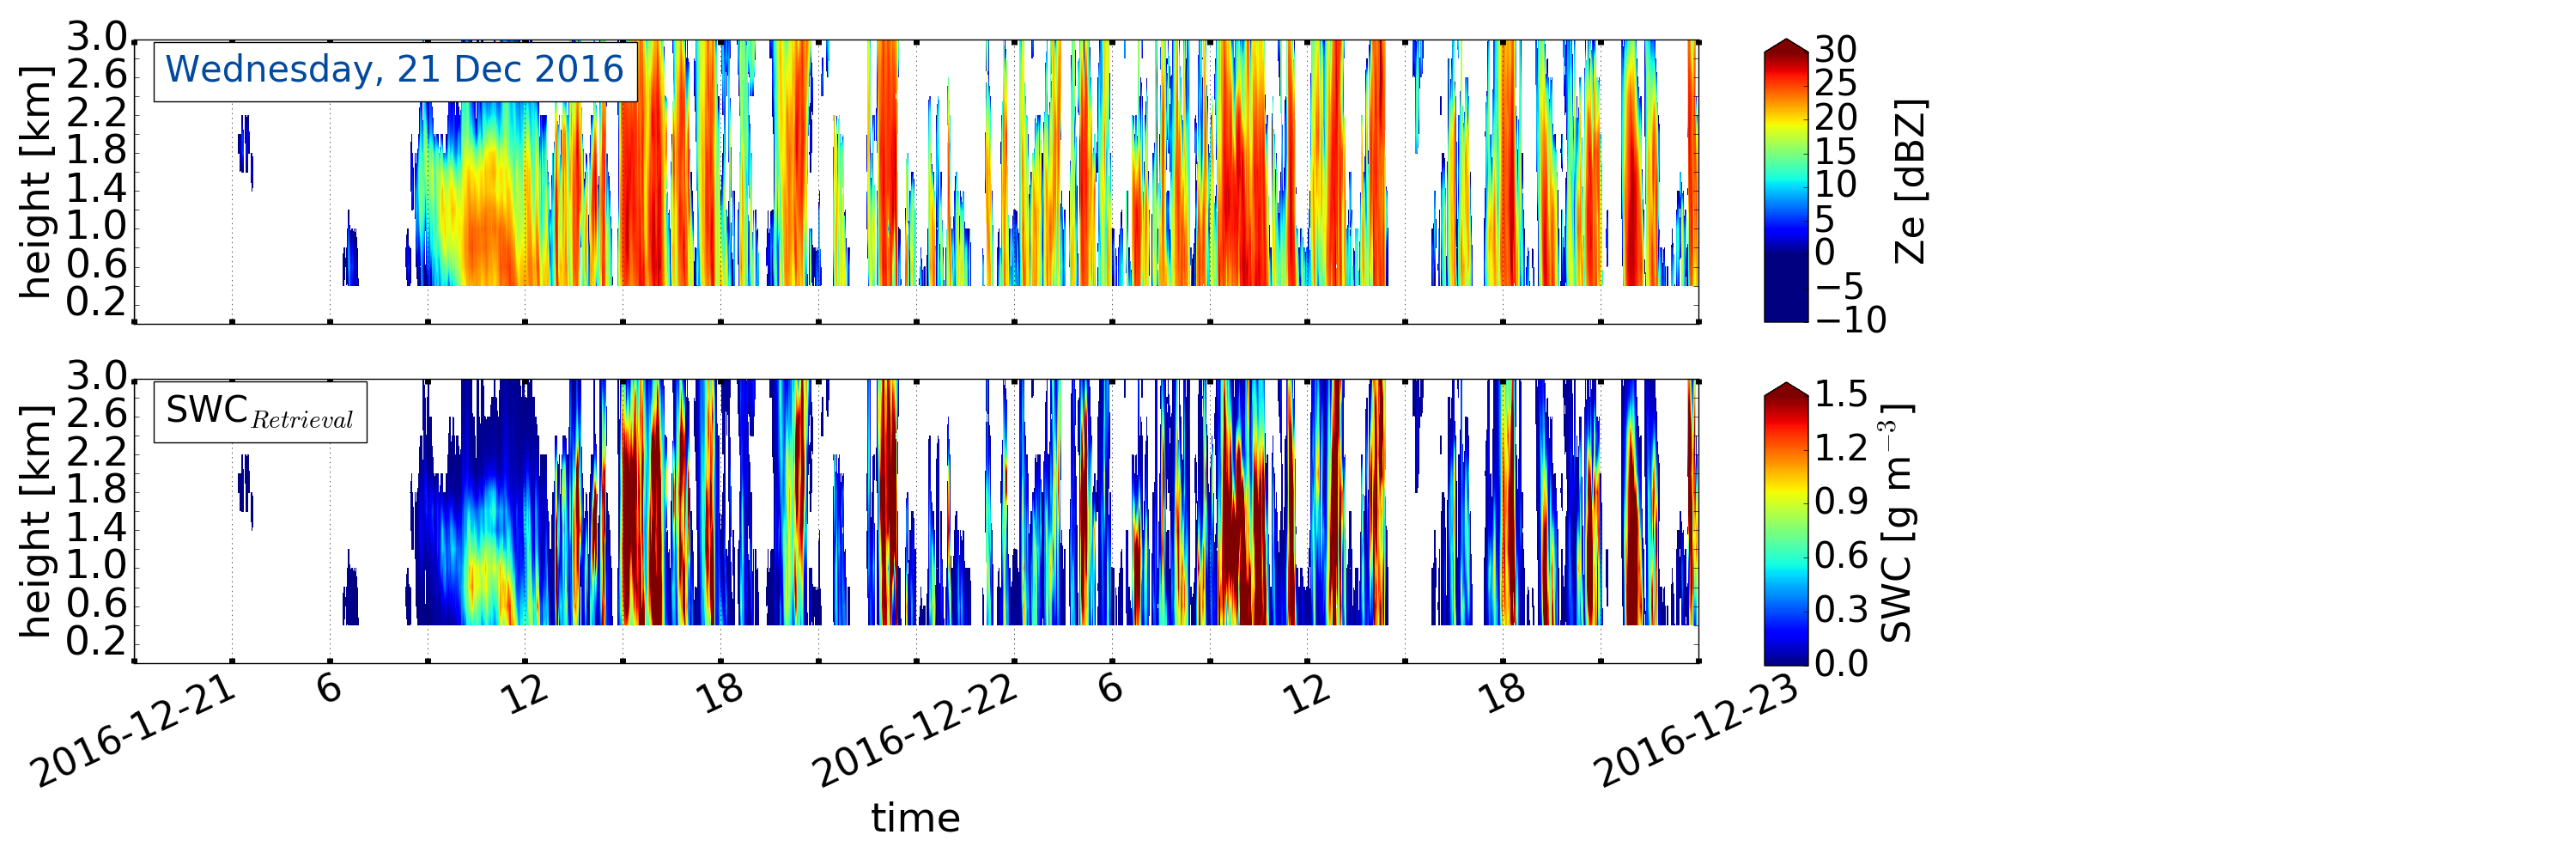
\includegraphics[trim={0.cm 2.2cm 19.cm 0.5cm},clip,width=0.9\textwidth]{./fig_obs_ret/20161221}
		\caption{}\label{fig:SWC:ret_21}
	\end{subfigure}
	% EM
	\begin{subfigure}[t]{\textwidth}
		\centering
		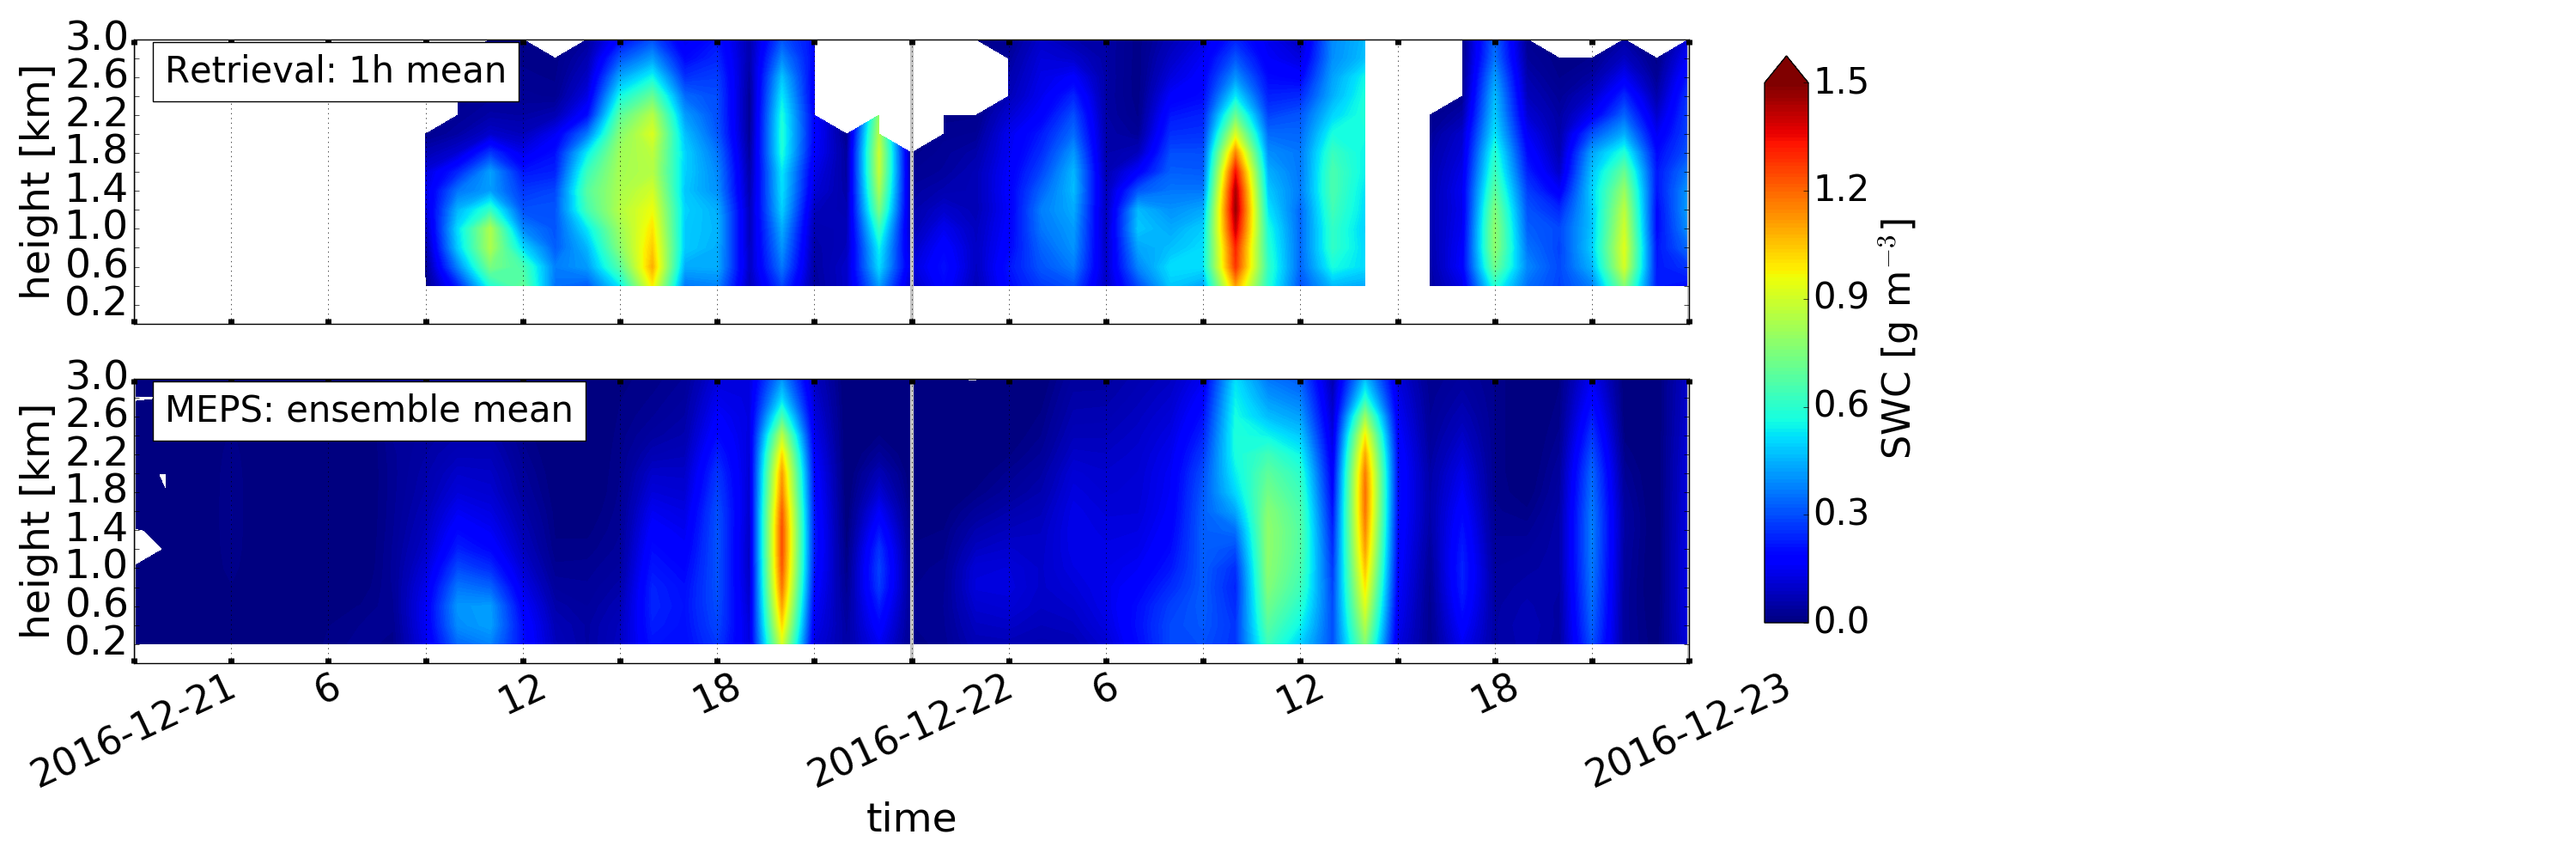
\includegraphics[trim={0.cm 2.2cm 19.cm 0.5cm},clip,width=0.9\textwidth]{./fig_vert_SWC_EM/20161221}
		\caption{}\label{fig:SWC_EM:21}
	\end{subfigure}
	% 3h
	\begin{subfigure}[t]{\textwidth}
		\centering
		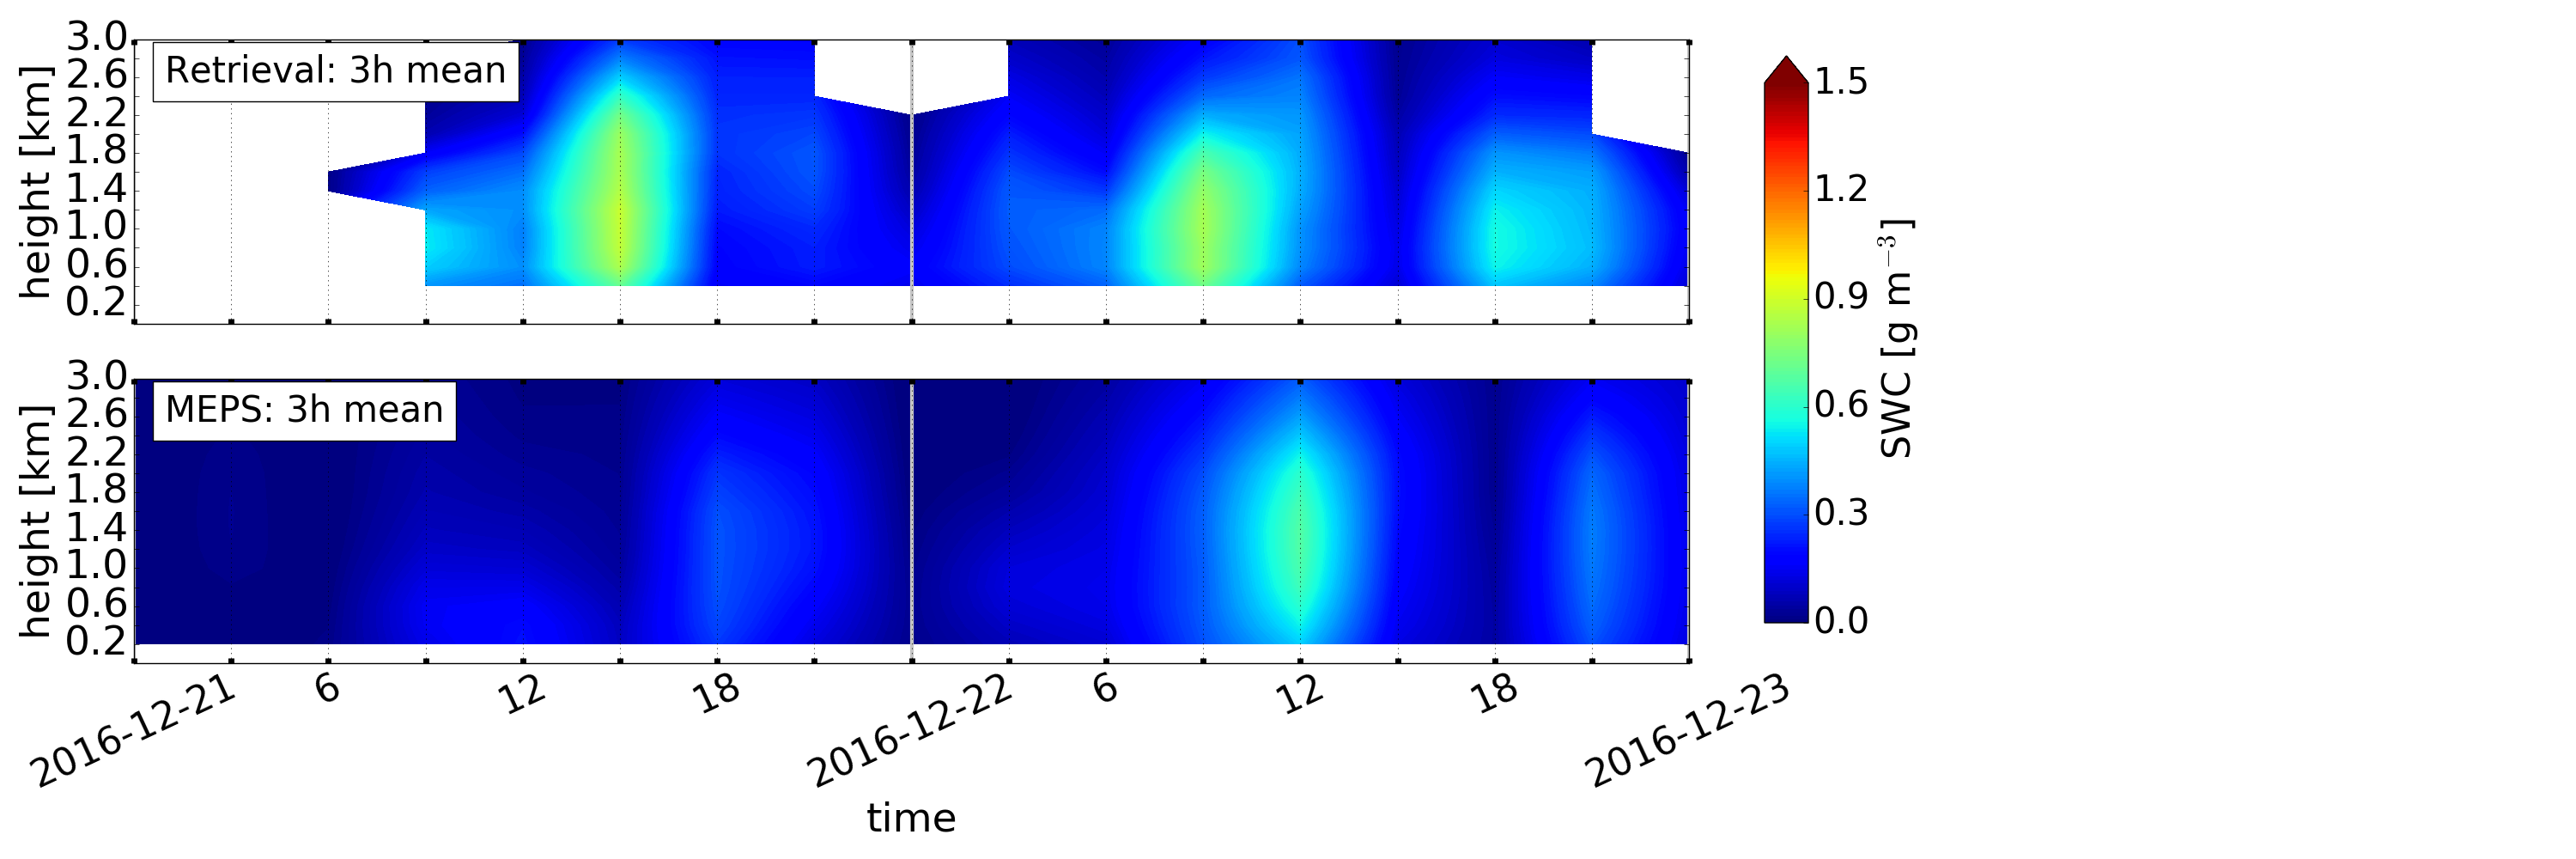
\includegraphics[trim={0.cm 0.8cm 19.cm 0.5cm},clip,width=0.9\textwidth]{./fig_vert_SWC_3h/20161221}
		\caption{}\label{fig:SWC3h:21}
	\end{subfigure}
	\caption{Initialisation \SI{21}{\dec} \SI{0}{\UTC}. 
		(\protect\subref{fig:SWC:ret_21},\protect\subref{fig:SWC:ret_24}) Upper panel: MRR reflectivity for \SI{48}{\hour}, lower panel minutely retrieved SWC. 
		(\protect\subref{fig:SWC_EM:21}, \protect\subref{fig:SWC_EM:24}) Upper panel: hourly averaged retrieved SWC, lower panel instantaneous hourly averaged forecast of all ensemble member SWC, neglecting missing values. 
		(\protect\subref{fig:SWC3h:21}, \protect\subref{fig:SWC3h:24}) Upper panel three hourly averaged retrieved SWC, lower panel instantaneous three hourly averaged forecast of all ensemble member SWC.   }\label{fig:ret:SWC21_24}
\end{figure}
%%%%%%%%%%%%%%%%%%%%%%%%%%%%%%%%%%%%%%%%%%%%%%
\noindent
\\
\\
As \Cref{fig:SWC_EM:21} indicates is the model able to cover almost the exact timing of the up-slope storm pattern. The variability of each ensemble member is presented in \Cref{fig:EM09_21}. It shows that almost all ensemble member agree on the occurrence of the storm pattern during \SIrange{9}{12}{\UTC}.
\\
Wind from the west and therefore over high mountains (\SI{1500}{\metre}) always follow a pulsing with more intense vertical precipitation e.g. on \SI{24}{\dec}, \Cref{fig:SWC:ret_24} and \ref{fig:SWC:ret_25}). 
This effect might be related to wave breaking at the mountain and result into a pulsing precipitation pattern. More precipitation events need to be studied to understand this effect around the Haukeliseter site. MEPS does not cover all pulses related to west wind during the course of a day. This is related to the short occurrence of the pulses as well as to the time resolution of the forecast values. Since the prediction values exist only every hour the model might miss some of the high pulses \SI{30}{\minute} before or after the frozen precipitation. 
\\
\\
One outcome of the presented study is that MEPS is able to resolve the local topography and predicts the wind direction correctly. The variability between the ensemble members is smaller for precipitation related to south-easterly winds (\Cref{fig:vari:EM22}, \subref{fig:vari:EM25}, \subref{fig:vari:EM26}). It did not cover the south-east wind direction on \SI{21}{\dec} (\Cref{fig:res:sfc_wd21}), which must be related to the local topography. 
\\
It seems more intuitive for the model to force large scale south-westerly flow into south direction rather than the observed wind direction along the south-easterly directed valley. As seen in \Cref{fig:res:topo} the wind must go along the \SI{7.2}{\degree} longitude, since a higher (\SIrange{1500}{1650}{\metre}) elevation is to the west and a \SI{1350}{\metre} high mountain to the east. True prediction of wind direction leads to the correct estimation of frozen precipitation patterns, such as up-slope (south-easterly wind) and pulsing (west wind). 
\\
\\
\Cref{sec:sfc_acc} describes the overestimation of surface snow accumulation during the intensification of the extreme storm. MEPS forecast in \Cref{fig:sfc_acc24}, \subref{fig:sfc_acc25}, and \subref{fig:sfc_acc26} show more ground accumulation than it is observed for \num{24} to \SI{26}{\dec}. One approach was to see, if the wind might have had an influence on the surface measurement of the double fence, which did not show to be true, even if \SI{10}{\percent} under-catch by the double fence gauge is assumed (\Cref{tab:res:MEPS_err_10}). A comparison of the hourly values of MEPS, show neither on \num{24} nor on \num{25} nor \SI{26}{\dec} high vertical snow amount compared to the estimated SWC (\Cref{fig:SWC_EM:24}, \ref{fig:SWC_EM:25}, and \subref{fig:SWC_EM:26}). \Cref{fig:EM09} shows values of very intense instatneous snow water content for individual ensemble members, but no prominent sign of overestimation when the surface miscalculation was present. 
\\
During \num{24} to \SI{26}{\dec} the wind was constantly from the west with higher wind speeds observed than during \num{21} to \SI{23}{\dec} (\Cref{fig:res:sfc_obs_meps}). \Cref{fig:scat:wd2123} and \subref{fig:scat:wd2426} indicate a better correlation for the forecasted and observed wind directions when precipitation overestimation occurred (\num{24} to \SI{26}{\dec}). During \num{24} and \SI{26}{\dec}, observed wind speeds were higher up to \SI{18}{\mPs} than on the previous days. As \Cref{fig:scat:ws2123} and \subref{fig:scat:ws2426} present is the correlation between observation and forecasts lower for high wind speeds. The high wind speeds from the west followed a pulsing storm pattern with changing intense and less intense snowfall (e.g. \num{22} and \SI{24}{\dec}, \Cref{fig:SWC:ret_22,fig:SWC_EM:22,fig:SWC3h:22}, \subref{fig:SWC:ret_24}, \subref{fig:SWC_EM:24}, \subref{fig:SWC3h:24}). MEPS is able to forecast the pulsing pattern for initialisations longer than \SI{24}{\hour} prior. Since the model estimates the wind direction correctly for west wind and local mountain affects it follows that there seems to be an interaction issue between frozen precipitation and the surface accumulation. Hourly vertical instantaneous values could have led to a misinterpretation of the here presented results. Furthermore, this study presents only a first look for a comparison between observed profiles of precipitation to MEPS forecast for an extreme event.   
\\
The ensemble variability in \Cref{fig:ens_vari} show that the ensemble members are divided about the existence of the exact precipitation pulsing. 
\\
\\
While the wind direction of MEPS has a good agreement, at least for west wind, shows the wind speed larger values over all days (\Cref{fig:scat:wd2123,fig:scat:wd2426,fig:scat:ws2123,fig:scat:ws2426}). Although MEPS includes ten perturbed ensemble members the insufficiency of AROME-MetCoOp too high wind prediction in extreme situations is not resolved. %The regional model wind prediction is still dependent on the intensity of the storm. 
As \cite{muller_arome-metcoop:_2017} mentioned are higher wind speeds in general better forecasted in AROME-MetCoOp than in ECMWF, which is an advantage for small scale forecast models. Especially in Norway, where the topography changes from sea to mountains. 
%%%%%%%%%%%%%%%%%%%%%%%%%%%%%%%%%%%%%%%%%%%%%%%%%%%%%%%%%%%%%%%%%%%%%%%%%%


